\begin{document}

\frontmatter

\title{CISM {\glimmerver} Documentation}
\author{
Stephen Price\thanks{Group T-3, Fluid Dynamics and Solid Mechanics, Los Alamos National Laboratory}, 
William Lipscomb\footnotemark[1],
Matthew Hoffman\footnotemark[1], \\
Magnus Hagdorn\thanks{School of GeoSciences, University of Edinburgh},
Ian Rutt\thanks{Department of Geography, Swansea University},
Tony Payne\thanks{School of Geographical Sciences, University of Bristol},
Felix Hebeler\thanks{Department of Geography, University of Zurich (original affiliation while working on project)}}

\maketitle

\chapter*{
\begin{center}
\textbf{\Large CISM2 Code Developers}
\end{center}
}

\author{Erin Barker (Los Alamos National Laboratory*),}
\author{Tim Bocek (University of Montana, Missoula*),}
\author{Josh Campbell (University of Montana, Missoula),}
\author{Katherine J. Evans (Oak Ridge National Laboratory),}
\author{Jeremy Fyke (Los Alamos National Laboratory*),}
\author{Glen Granzow (University of Montana, Missoula),}
\author{Magnus Hagdorn (School of GeoSciences, University of Edinburgh),}
\author{Brian Hand (University of Montana, Missoula*),}
\author{Felix Hebeler (University of Zurich*),}
\author{Matthew Hoffman (Los Alamos National Laboratory),}
\author{Jesse Johnson (University of Montana, Missoula),}
\author{Irina Kalashnikova (Sandia National Laboratories),}
\author{Joseph H. Kennedy (Oak Ridge National Laboratory),}
\author{Jean-Francois Lemieux (New York University*),}
\author{William Lipscomb (Los Alamos National Laboratory),}
\author{Daniel Martin (Lawrence Berkeley National Laboratory),}
\author{Jeffrey A. Nichols (Oak Ridge National Laboratory),}
\author{Ryan Nong (Sandia National Laboratories*),}
\author{Matthew R. Norman (Oak Ridge National Laboratory),}
\author{Tony Payne (University of Bristol),}
\author{Stephen Price (Los Alamos National Laboratory),}
\author{Doug Ranken (Los Alamos National Laboratory),}
\author{Ian Rutt (Department of Geography, Swansea University),}
\author{William Sacks (National Center for Atmospheric Research),}
\author{Andrew Salinger (Sandia National Laboratories),}
\author{James B. White III (Oak Ridge National Laboratory*),}
\author{Jon Wolfe (National Center for Atmospheric Research*),}
\author{Patrick Worley (Oak Ridge National Laboratory),}
\author{Timothy Wylie (University of Montana, Missoula*),}

\textit{* author's original affiliation while working on project}

\chapter*{
\begin{center}
\textbf{\Large Funding}
\end{center}
}

The development of CISM has been supported by the U.K. National Environmental Research Council (through the Centre for Polar and Ocean Modelling), 
the U.S. National Science Foundation (through the Office of Polar Programs), and the U.S. Department of Energy (through the Office of Science, Biological 
and Environmental Research and Advanced Scientific Computing Research Programs).

\tableofcontents

\ifthenelse{\boolean{html}}
{
\Configure{graphics*} 
         {eps} 
         {\Needs{"convert \csname Gin@base\endcsname.eps 
                               \csname Gin@base\endcsname.png"}% 
          \Picture[pict]{\csname Gin@base\endcsname.png}% 
         } 

}
{}

\mainmatter
\part{User Documentation}

\chapter{Introduction and Overview}
\newcommand{\dir}{intro}
\label{ch:runcism}

\section{Overview of Running CISM}

Assuming you successfully completed the Installation instructions in Chapter \ref{chp:install},
the executable for running the model, \texttt{cism\_driver}, can be found in your 
build directory in a subdirectory called \texttt{cism\_driver} 
(e.g., \texttt{./builds/mac-gnu/cism\_driver/cism\_driver}).

The build system creates the executable at this path but does not automatically
make it available to other locations on your system.  How you choose to do so depends 
on your situation.  See the introduction to Chapter \ref{chp:testcases} for 
an overview of how to make the executable available to other locations on your system
(e.g., symlinking, copying, or modifying your PATH environment variable).

Unlike previous versions of Glimmer, with CISM 2.0 this single \texttt{cism\_driver} 
executable is used for running the model in all configurations.
\texttt{cism\_driver} can be invoked with a single argument specifying 
a CISM .config file to run CISM as a standalone ice sheet model without Glint climate forcing,
or with two arguments (a CISM config file and a Glint config file) 
to run CISM with Glint climate forcing:
\begin{verbatim}
 Call cism_driver with either 1 or 2 arguments. Examples:
 cism_driver ice_sheet.config
 cism_driver ice_sheet.config climate.config
\end{verbatim}
The available options for the CISM configuration file and 
for the Glint climate interface configuration file are described in detail below.

To perform a parallel run with the parallel build of CISM, you must use the
MPI run command, which is typically \texttt{mpirun} or \texttt{mpiexec} but may 
vary among MPI versions and installations.  A standard syntax that is likely to
work on most installations is \newline
 \indent \texttt{mpirun -np N cism\_driver ice\_sheet.config \textit{climate.config}} \newline
where \texttt{N} is the number of processors you want to use, \texttt{ice\_sheet.config} is the name of the CISM
configuration file, and the optional argument \texttt{\textit{climate.config}} is the name 
of the climate configuration file.  For example: \newline
 \indent \texttt{mpirun -np 4 cism\_driver dome.config}\newline
would run the dome test case on four processors.

Finally, note that instructions for running CISM within the Community Earth System Model (CESM)
or another climate model are not described here.

When CISM runs, some basic information about its operation will be output to 
the screen (standard out).  More verbose information about the run will be written 
to a log file which is named \texttt{\textit{ice\_sheet.config}.log} where 
\texttt{\textit{ice\_sheet.config}} is the name of the .config file use to perform
the run.  (For example, if running the model with  \texttt{./cism\_driver dome.config},
the log file will be called  \texttt{dome.config.log}.)  The log file is an
important reference, especially for debugging runs that do not behave as expected.
For example, the log file includes a list of configuration options and parameter
values, which can be useful in diagnosing problems like typos in your .config file.
The log file also indicates what files were used for input and output and at which
times I/O occurred.  The log file may contain warnings about potentially
problematic configuration combinations or model behavior, such as the use of
configurations settings that are not scientifically validated, or a CFL violation
during advection.  In contrast, fatal errors will kill the model and the error
message will be written to both the screen and the log file.

Optionally, the log file also contains diagnostic information about the global
state of the ice sheet (e.g., the total ice area and volume, the maximum surface and basal
speeds, and the max and min temperatures), along with vertical profiles of speed
and temperature at a user-specified grid point.  This information is written at intervals
specified by the config file variable \texttt{dt\_diag}, for the diagnostic
point \texttt{(idiag,jdiag)}.

In addition to the log file, the model will create any netCDF output files requested
in the config file (see Section \ref{io-config} below for details).  
If the model dies for some reason midway through a simulation,
the netCDF files will still include output for the portion of the simulation that 
was completed.

\section{Overview of Configuration Files}

Running CISM is managed through configuration files (*.config) that enable 
desired model features and control input of initial conditions and forcing 
and output of model results.  This chapter summarizes the configuration options 
available for running CISM and is divided into sections on general Model Configuration, 
Input/Ouput Configuration, and optional Climate Forcing Configuration.

The format of CISM configuration files is taken from that used by the 
ConfigParser module in Python 2.x, which is similar to Windows \texttt{.ini} files 
and contains sections. Each section contains key/value pairs.

\begin{itemize}
\item[Comments:] Empty lines, or lines starting with a \texttt{\#}, \texttt{;} or \texttt{!} are ignored.  Comments can also be added on the same line as a key/value pair using these delimiters.
\item[Sections:] A new section starts with the section name enclosed by square brackets, \texttt{[ ]} and can be up to 50 characters long, e.g., \texttt{[grid]}.
\item[Key/Value Pairs:] Keys are separated from their associated values by \texttt{=} or \texttt{:}. The names can be up to 50 characters long. Values can be up to 400 characters long.
\end{itemize}

Sections and keys are case-sensitive and may contain white space. 
However, the configuration parser is very simple and thus the number of spaces 
within a key or section name also matters. Sensible defaults are used when 
a specific key is not found; defaults are shown in bold in the tables below.

Here is an example configuration file:
\begin{verbatim}
;a comment
[a section]
an_int  : 1
a_float = 2.0
a_char  = hey, this is rather cool
an_array = 10. 20. -10. 40. 100.

[another section]
! more comments
foo : bar
\end{verbatim}





\chapter{Installing CISM}
\label{chp:install}
\renewcommand{\dir}{install}
\input{\dir/install.tex}

\chapter{Introduction to Ice Sheet Modeling: Derivation of Field Equations}
\renewcommand{\dir}{modeling-intro}

In this chapter we give an introduction to ice dynamics and the governing conservation equations.

\section{Conservation of Momentum}


Starting from Newton's second law of motion, conservation of momentum is

\begin{equation}
\frac{d} {dt} \int_{V}\rho u_{i}~dV ~ = ~ \int_{V} \frac{\partial \sigma_{ij}} {\partial x_{j}} ~dV +  \int_{V} \rho g_{i}~dV
\end{equation}

where $t$ represents time, $\rho$ represents density, $u$ represents
velocity, $\sigma_{ij}$ represents the stress tensor, $g$ represents the
acceleration due to gravity, $V$ represents the volume of an arbitrary
fluid element, and $(i,j)= \{x, y, z\}$ in a cartesian coordinate
system. Equation \textbackslash{}ref\{equation:mobal1\} tells us that a
fluid element of arbitrary size experiences a ``body force''
$\rho g_{i}\delta V$ due to gravity and a force
$\frac{\partial \sigma_{ij}} {\partial x_{j}} \delta V$ due to the
surrounding fluid.

Making the assumptions that we have continuous fields and that ice is
incompressible (that is, its density $\rho$ does not change under
conditions of interest to us), we can write

\begin{equation}
\rho \frac{D u_{i}}{D t}~=~\frac{\partial \sigma_{ij}}{\partial x_{j}} + \rho g_{i}
\end{equation}

in which $D$ is a material derivative. Due to the fact that Froude
number \href{Wikipedia:Froude number}{Wikipedia:Froude number} for ice
flow is extremely small, the acceleration term (the first term on the
left hand side) could be neglected and we arrive to a steady-state form.

\begin{equation}
\frac{\partial \sigma_{ij}}{\partial x_{j}} + \rho g_{i} ~=~0
\end{equation}

We are left with the very simple statement that the gravitational
driving force is balanced by forces resulting from the stresses
$\sigma_{ij}$.

The stress tensor $\sigma_{ij}$ has nine components in our three
dimensional cartesian coordinate system

\begin{equation}
\mathbf{\sigma} =
\left\vert  \begin{array}{ccc} 
    \sigma _{ xx} & \sigma _{ xy} & \sigma _{ xz} \\
    \sigma _{ yx} & \sigma _{ yy} & \sigma _{ yz} \\
    \sigma _{ zx} & \sigma _{ zy} & \sigma _{ zz} \\
\end{array} \right\vert 
\end{equation}

The components along the diagonal are called normal stresses and the
off-diagonal components are called shear stresses. Deformation results
not from the full stress but from the deviatoric stress

\begin{equation}
\tau_{ ij} ~ = ~ \sigma _{ ij} ~ - ~{\frac{ 1}{ 3}} \sigma _{ kk} \delta _{ ij}
\end{equation}

in which $\delta_{ ij}$ is the Kroneker delta.

\subsubsection{Constitutive relationship}

Strain rates $\dot{\epsilon}_{ij}$ are related to the stress tensor
$\tau_{ij}$ by the generalized Glen flow law

\begin{equation}
\dot{\epsilon}_{ij}~=~A(T^{*})\tau_{e}^{n-1}\tau_{ij}
\end{equation}

in which $T^{*}$ is the absolute temperature corrected for the pressure
dependence of the melt temperature, $\tau_{e}$ is the second invariant
of the stress tensor and the exponent $n$ is 3. The rate factor $A$
follows the Arrhenius relationship

\begin{equation}
A\left( T^{*}\right)~=~E A_{o}e^{-Q/RT^{*}}
\end{equation}

in which $A_{o}$ is a constant, $Q$ represents the activation energy for
crystal creep, $R$ is the gas constant, and $E$ is a tuning parameter
used to account for the effects of impurities and anisotropic ice
fabrics. The homologous temperature is

\begin{equation}
T^{*}=T+\rho g H \Phi
\end{equation}

in which $\Phi$ is 9.8 $\times$10$^{-8}$ K Pa$^{-1}$, about 8.7
$\times$10$^{-4}$ K m$^{-1}$. The pressure-dependent melt temperature is
simply the triple point temperature less the product $\rho g H \Phi$.

\section{Conservation of Energy}


The first law of thermodynamics is used to make a basic statement of
conservation of energy in a volume of ice V within a surface S is

\begin{equation}
\frac{d}{d t} \int_{V}E ~dV~=~- \int_{S}\mathbf{F}\cdot \hat{n}~dS~-~\int_{S}E \mathbf{u}\cdot \hat{n}~dS~+~\int_{V}W dV
\end{equation}

in which $E$ represents the energy of the volume, $F_{i}$ is a flux due
to diffusion, and $W$ represents any sources or sinks of energy within
the volume. The term $Eu_{i}$ is a flux through $S$ due to advection.
Following the steps laid out earlier, we use the divergence theorem and
the assumptions of continuous fields and incompressibility, such that

\begin{equation}
\frac{dE}{dt}~+~\nabla \cdot \left(F_{i} +E u_{i}  \right)~-~W~=~0
\end{equation}

Our goal is to use the first law of thermodynamics in order to compute
the temperature of the ice and any change it may undergo over time.

The energy $E$ is the product of density and the specific internal
energy of the ice $e$, which is itself the product of the specific heat
capacity $c_{p}$ and temperature $T$ because there is no transfer
between internal energy and pressure for an incompressible fluid. Thus,

\begin{equation}
\begin{matrix}
\frac{dE}{dt}&=&\frac{d\left(\rho e \right)}{dt} \\
&=&\rho\frac{de}{dt}~+~e \frac{d\rho}{dt}\\
&=&\rho c_{p} \frac{dT}{dt}
\end{matrix}
\end{equation}

The flux due to diffusion follows Fourier's ``law'' for heat conduction
so

\begin{equation}
\begin{matrix}
\nabla \cdot F_{i}&=&\nabla \cdot \left( -k ~\nabla T  \right) \\
&=&-k~\nabla^{2}T
\end{matrix}
\end{equation}

in which $k$ represents the thermal diffusivity of ice and we assume
gradients in its magnitude to be negligible.

Using progress made above and assuming that $\nabla \cdot u_{i}$ is
small with respect to other terms, we can write the advection term

\begin{equation}
\begin{matrix}
\nabla \cdot \left(E u_{i} \right)~=~\rho c_{p}~ u_{i} \cdot \nabla T  
\end{matrix}
\end{equation}

Two quantities must be considered as energy sources, the work done on
the system by internal deformation and the latent heat associated with
phase changes. The former is the product of strain rate and the
deviatoric stress $\dot{\epsilon}_{ij} \tau_{ij}$. The latter is the
product of the latent heat of fusion and the amount of material subject
to melting (freezing) per unit volume per unit time, $L_{f}M_{f}$.

At last, we are able to write equation
\textbackslash{}ref\{equation:enbal2\} in terms of temperature

\begin{equation}
\frac{\partial T}{\partial t}~=~\frac{k}{\rho c_{p}} \nabla^{2}T~-~u_{i}\cdot \nabla T~+~\frac{1}{\rho c_{p}} \dot{\epsilon}_{ij} \tau_{ij} ~+~\frac{1}{\rho c_{p}} L_{f} M_{f}
\end{equation}

It is often the case that horizontal terms
$\frac{\partial^{2} T}{\partial x^{2}}$ and
$\frac{\partial^{2} T}{\partial y^{2}}$ are small enough to be ignored.

\subsection{Conservation of Mass}

In this case, $\phi$ from our general conservation equation represents the mass $M$, or more conveniently
$M = \int_V \rho dV$, the integral of the density over the volume. Assuming that there are no sources or 
sinks of mass in the volume ($R$=0), the mass conservation equation is written

\begin{equation}
\int_{V}\frac{\partial \rho} {\partial t} ~dV ~+~ \int_{V} \nabla \cdot \rho \mathbf{u} dV~=~0
\label{eq:mascon1}
\end{equation}

\noindent
Ice is incompressible (the density does not change in time), which provides the equation for 
local mass continuity,

\begin{equation}
\nabla \cdot \mathbf{u} ~=~0.
\label{eq:mascon2}
\end{equation}

\noindent
Equation \eqref{eq:mascon2} says that the velocity field is divergence-free. Applying the $\nabla$ 
operator in Cartesian coordinates gives

\begin{equation}
\frac{\partial u_{x}}{\partial x}~+~\frac{\partial u_{y}}{\partial y} ~+\frac{\partial u_{z}}{\partial z}~=~0.  
\label{eq:mascon3}
\end{equation}

\noindent
To make use of this statement, we need to integrate from the base $b$ to the upper surface $s$ of the ice mass,

\begin{equation}
\int_{b}^{s} \left( \frac{\partial u_{x}}{\partial x}~+~\frac{\partial u_{y}}{\partial y} ~+\frac{\partial u_{z}}{\partial z}\right) dz~=~0.  
\label{eq:mascon4}
\end{equation}

\noindent
The integral of $\frac{\partial u_z}{\partial z}$ is simply the difference between
the vertical component of the velocity at the upper and lower surfaces, so

\begin{equation}
u_{z} \left(s\right)-u_{z} \left(b\right)~=~-\int_{b}^{s} \frac{\partial u_{x}}{\partial x} dz ~-~\int_{b}^{s} \frac{\partial u_{y}}{\partial y} dz.  
\label{eq:mascon5}
\end{equation}

\noindent
Changing the order of integration and differentiation using 
\href{http://en.wikipedia.org/wiki/Leibniz_integral_rule}{Leibniz's rule}, we obtain

\begin{equation}
\begin{matrix}
u_{z} \left(s\right)-u_{z} \left(b\right) & = & -~\frac{\partial}{\partial x} \int_{b}^{s} u_{x} dz ~ +~u_{x}(s)\frac{\partial s}{\partial x} ~-~ u_{x}(b)\frac{\partial b}{\partial x}  \\ 
& & -~\frac{\partial}{\partial y}\int_{b}^{s} u_{y} dz   ~ +~u_{y}(s)\frac{\partial s}{\partial y} ~-~ u_{y}(b)\frac{\partial b}{\partial x}.
\end{matrix}
\label{eq:mascon6}
\end{equation}

The vertical velocity at the upper surface $u_{z}(s)$ is the result of motion parallel to the surface slope, 
the rate of new ice accumulation $B_s$, and any time-change in the surface height,

\begin{equation}
u_{z} \left(s\right)~=~\frac{\partial s}{\partial t}~+~u_{x}(s)\frac{\partial s}{\partial x}~+~u_{y}(s)\frac{\partial s}{\partial y}~-~B_s, 
\label{eq:mascon7}
\end{equation}

\noindent
recognizing that a negative accumulation rate indicates ablation. Similarly, the vertical velocity at the lower surface is

\begin{equation}
u_{z} \left(b\right)~=~\frac{\partial b}{\partial t}~+~u_{x}(b)\frac{\partial b}{\partial x}~+~u_{y}(b)\frac{\partial b}{\partial y}~-~B_b
\label{eq:mascon8}
\end{equation}

\noindent
in which $B_b$ is the basal accumulation rate.
Substituting \eqref{eq:mascon7} and \eqref{eq:mascon8} into \eqref{eq:mascon6}, we find that many terms cancel:

\begin{equation}
\frac{\partial s}{\partial t}~-~B_s~-~\frac{\partial b}{\partial t}~+~B_b~=~-~\frac{\partial}{\partial x} \int_{b}^{s} u_{x} dz~-~\frac{\partial}{\partial y} \int_{b}^{s} u_{y} dz.
\label{eq:mascon9}
\end{equation}

\noindent
Finally, making the substitution that the ice thickness $H=s-b$, we obtain

\begin{equation}
\frac{\partial H}{\partial t}~=~-~\frac{\partial}{\partial x} \int_{b}^{s} u_{x} dz~-~\frac{\partial}{\partial y} \int_{b}^{s} u_{y} dz ~+~B_s~+~B_b.
\label{eq:mascon10}
\end{equation}

\noindent
Integrating in the vertical gives

\begin{equation}
\frac{\partial H}{\partial t}~=~-~\nabla \cdot \left( U_{i} H \right) +~B_s~+~B_b,
\label{eq:mascon11}
\end{equation}

\noindent
in which $U_{i}$ is the vertically averaged velocity, i.e., $U_i = \frac{1}{H}\int_{b}^{s}u_{i}dz$ . Equation \eqref{eq:mascon11} is 
prognostic; we can use the current velocity and geometry of the ice to compute the rate of change in the geometry.




\chapter{Shallow Ice Dynamics: Glide Dynamical Core}
\renewcommand{\dir}{shallow-ice}
\label{ch:glide}

This chapter describes the numerical implementation of mass, momentum, and energy conservation in the Glide dynamical core. For a model governed by shallow-ice dynamics, the solutions for the conservation of mass and momentum are intimately linked.

\input{\dir/kinematics.tex}
\input{\dir/temp.tex}
\section{Basal Boundary Condition}
This section describes the formulation of the basal boundary condition.
An interface for the upper boundary condition (atmospheric BC) is easily defined by the surface temperature and mass balance. Similarly, the basal boundary consists of mechanical and thermal boundary conditions. The complications arise because the thermal and mechanical boundary conditions depend on each other. The interface of the basal boundary can be described with the following fields (see also Fig. \ref{num.fig.basal_bc}):
\begin{enumerate}
\item \textbf{basal traction:} This field specifies a parameter which is used to allow basal sliding.
\item \textbf{basal heat flux:} This is the heat flux entering the ice sheet from below.
\item \textbf{basal water depth:} The presence of basal melt water affects the basal ice temperature.
\end{enumerate}
Also, the ice sheet model calculates a melt/freeze rate based on the temperature gradient and basal water depth. This is handled by Glide.

\begin{figure}[htbp]
  \centering
  
\includegraphics[width=0.9\textwidth]{\dir/figs/basal_bc.eps}
  \caption{Basal boundary condition.}
  \label{num.fig.basal_bc}
\end{figure}

\subsection{Mechanical boundary conditions}
If the ice is not frozen to the bed, basal d\'{e}collement may occur. This can be parameterized by a traction factor, $t_b$. 
Within the ice sheet model, $t_b$ can be used to calculate basal sliding velocities $\vec{u}_b$ in the case of zero--order physics. That is,
\begin{equation}
  \vec{u}_b=t_b\vec{\tau}_b,
\end{equation}
where $\tau_b$ is the basal shear stress. Alternatively, $t_b$ can be used as part of the stress--balance calculations when the model is used with higher order physics. In simple models $t_b$ may be uniform or prescribed as a spatial variable. More complex models may wish to make $t_b$ dependent on other variables, such as basal melt rate. Typically $t_b$ will depend on the presence of basal water.

The second mechanical boundary condition, basal melting/freeze--on $M_b$, is handled within the ice sheet model. The details are described in Section \ref{num.sec.bc_melt}.

\subsection{Thermal boundary conditions}
The thermal boundary condition at the ice base is more complicated than the mechanical BC. The ice is heated from below by the geothermal heat flux. Heat is generated by friction with the bed. Furthermore, the ice temperature is constrained to be less than or equal to the pressure melting point of ice. The thermal boundary condition is a flux condition if there is no water present. If there is water, the basal temperature is set to the pressure melting temperature. (If it were lower, there would be no water, and if it were higher, there would be no ice.)

\subsubsection{Basal melting and freezing}\label{num.sec.bc_melt}
At the ice base, $z=b$, we can define outgoing and incoming heat fluxes, $H_o$ and $H_i$:
\begin{subequations}
  \begin{align}
    H_o&=-k_{\text{ice}}\left.\frac{\pd T}{\pd z}\right|_{z=b^+}\\
    \intertext{and}
    H_i&=-k_{\text{rock}}\left.\frac{\pd T}{\pd z}\right|_{z=b^-}+\vec{u}_b\cdot\vec{\tau}_b+
    \begin{cases}
      {\rho_{\text{ice}}M_b}/{L} & \text{when $M_b<0$} \\
      0 & \text{otherwise}
    \end{cases}
  \end{align}
\end{subequations}
where $k_{\text{ice}}$ and $k_{\text{rock}}$ are the thermal conductivities of ice and rock, $\vec{u}_b\cdot\vec{\tau}_b$ is the heat generated by friction with the bed, and $L$ is the latent heat of fusion. The basal melt/freeze--on rate $M_b$ can then be calculated from the difference between the incoming and outgoing heat fluxes:
\begin{equation}
  \label{bc.eq.meltrate}
  M_b=\frac{H_i-H_o}{\rho_{\text{ice}}L}
\end{equation}
There is freeze--on if $M_b < 0$, and basal melting if $B_b > 0$.

\input{\dir/gthf.tex}

\subsection{Basal hydrology}
It is clear from the discussion above that the presence of basal water plays a crucial role in specifying both the mechanical and thermal boundary conditions. However, the treatment of basal water can vary greatly. Basal water is, therefore, left as an unspecified interface. Glide does provide a simple local water balance model which can be run in the absence of more complex models.

\subsection{Putting it all together}
The basal boundary consists of the individual components described in the previous sections. All components are tightly linked with each other. Figure \ref{num.fig.bc_flow} illustrates how the modules are linked and in what order they are resolved.
\begin{figure}[htbp]
  \centering
  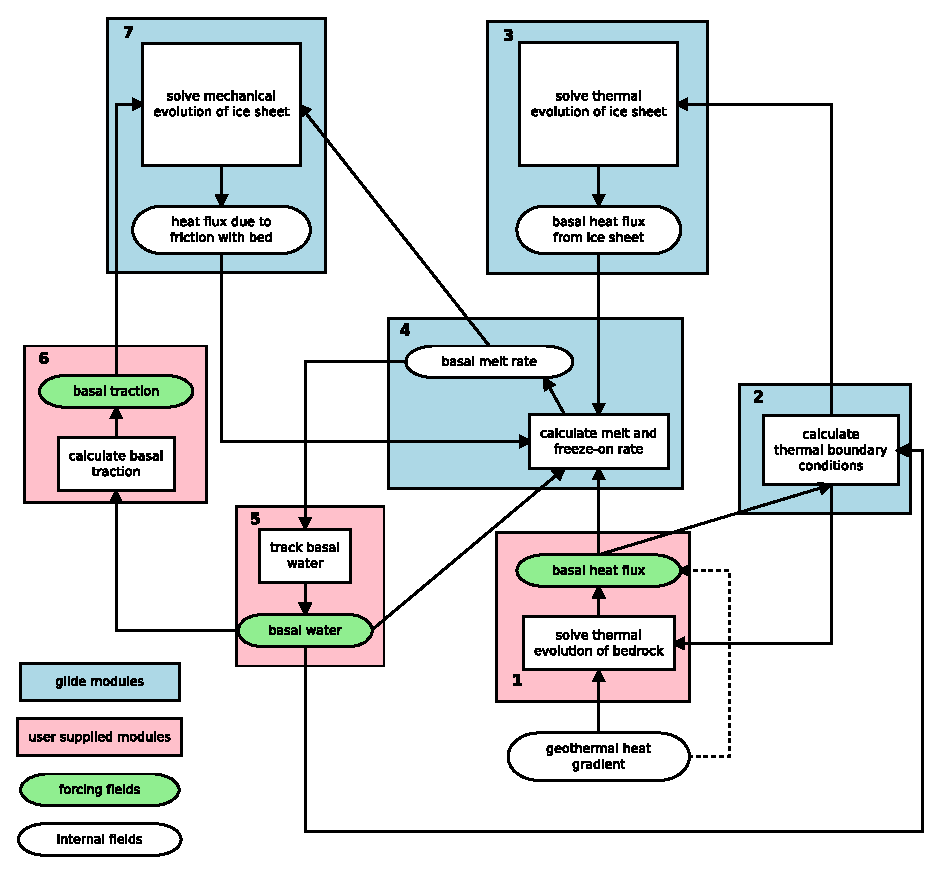
\includegraphics[width=\textwidth]{\dir/figs/basal_alg.eps}
  \caption{Flow diagram illustrating how the various modules communicate with each other by exchanging data fields.}
  \label{num.fig.bc_flow}
\end{figure}
The order of executions is then:
\begin{enumerate}
\item Find the basal heat flux by either solving the equation describing the thermal evolution of the lithosphere, \eqref{num.eq.diffu_rock}, or by using the geothermal heat flux directly. The upper boundary condition of \eqref{num.eq.diffu_rock} is the same as the lower boundary condition of the thermal evolution of the ice sheet.
\item Either (1) the lower boundary condition for the thermal evolution of the ice sheet is given by the basal heat flux from \emph{Step 1}; or (2) if melt water is present, the basal temperature is set to the pressure melting point of ice.
\item Calculate the temperature distribution within the ice sheet given the boundary condition found during \emph{Step 2} and the atmospheric BC.
\item Calculate a melt/freeze--on rate using Equation \eqref{bc.eq.meltrate} given the outgoing heat flux calculated during \emph{Step 3}, friction with the bed (calculated during the previous \emph{Step 7}) and the incoming heat flux from \emph{Step 1}. Freezing occurs only when there is basal water.
\item Track basal water. This is a user supplied module which can take any complexity. Inputs will typically be the melt/freeze--on rate determined during \emph{Step 4}.
\item Calculate the basal traction parameter. Again, this is a user supplied module which typically will involve the presence of basal water (calculated during \emph{Step 5}).
\item Solve the mechanical ice equations given basal traction parameter from \emph{Step 6}.
\end{enumerate}
Clearly, this scheme has the problem that heat is lost if the basal heat flux is such that more water could be frozen than is available. This might be avoided by iterating the process. On the other hand, the heat loss may be negligible if time steps are fairly small.

\input{\dir/isos.tex}


% ==========================
% MJH: An additional section not worth adding a new file for

\section{Time Step Ordering}

Relative to Glimmer-CISM 1.x, the order of operations on each time step has been
somewhat reorganized in CISM2.0.  This was done for consistency with the ordering
of operations used in Glissade and to eliminate discrepancies between time levels
applied in the model and the time levels written in output files.  
\textbf{These changes have only a minor impact on model results, but do result 
in output that will not be an exact match between the two model versions for the
same configuration and initial conditions.}

While unlikely to be of much interest to the average user, particularly if you are not
migrating from Glimmer-CISM 1.x, the details of these changes follow.
Specifically, in Glimmer-CISM 1.x, for a given time step, $H$ is advanced in time
relative to $T$ and $\vec{v}$, and, because a complete solve occurs even at the 
initial time, the output for the initial time is different than the input for 
the prognostic variables $H$ and $T$, even though no time step has occurred at 
that point.

In Glimmer-CISM 1.x, the time-stepping loop is organized as follows:
\begin{verbatim}
glide_initialise(): init T, H, v
do while (t < tend)
   glide_tstep_p1(): solve T
   glide_tstep_p2(): solve v, H
   glide_tstep_p3(): calculate some diagnostic variables, write output for time t
   advance time
end do
\end{verbatim}

\noindent This results in the following relation between the state of model variables and
the time level at which they are output:

%\begin{table}[h]
%\caption{Relation between state of model variables and output time level in Glimmer-CISM 1.x}
\begin{tabular}{lccc}
\hline
Output time:  & 0    & 1   & 2  \\
\hline
$T$  &  1                    &  2                    &  3  \\
$H$  &  1                    &  2                    &  3  \\
$v$  &  0                    &  1                    &  2  \\
\hline
\end{tabular}
%\end{table}
\\~\\  % hack to get a little more vertical separation here

In CISM 2.0, the time-stepping loop is now organized as follows:
\begin{verbatim}
initialize modules
initial diagnostic solve of v (and any other diagnostic variables like upper surface)
write output for time 0
do while (t <= tend)
   advance time
   solve column physics: T = f(H,T) 
   solve prognostic variables: advection of H=f(H,v), T=f(H,v)
   solve diagnostic variables: v=f(H,T)
   write output for time t
end do
\end{verbatim}

\noindent
This results in the following relation between the state of model variables and
the time level at which they are output:

%\begin{table}[h]
%\caption{Relation between state of model variables and output time level in CISM 2.0}
\begin{tabular}{lccc}
\hline
Output time:  & 0    & 1   & 2  \\
\hline
$T$  &  0                    &  1                    &  2  \\
$H$  &  0                    &  1                    &  2  \\
$v$  &  0                    &  1                    &  2  \\
\hline
\end{tabular}
%\end{table}




\chapter{Introduction to Higher-Order Ice Dynamics}
\renewcommand{\dir}{higher-order}

\label{ch:higher-order}


\section{Higher-Order Dynamics in CISM}
\label{sc:higher-order-into}

\subsection{Basics}
The main distinction between so-called higher-order models and 0-order (or ``shallow ice") models is that higher-order models attempt a closer approximation to solving the non-linear Stokes equations. In general, this usually means incorporating some approximation of horizontal-stress gradients -- along-flow stretching or compression and across-flow shearing -- in addition to the vertical stress gradients that are accounted for in shallow ice models (Figure \ref{fig:stressbalance}). This is important for several reasons:

\begin{figure}
  \begin{center}
    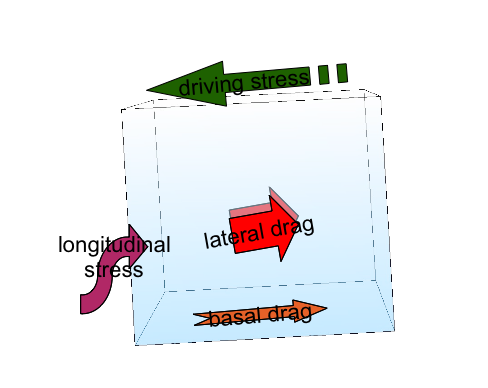
\includegraphics[width=0.5\columnwidth]{\dir/figs/StressBalance.eps}
  \end{center}
  \caption{The gravitational stress available to move the ice is the driving stress, indicated in green. Because the ice is assumed to be in equilibrium, the sum of the other stresses is equal to (i.e., must balance) the gravitational driving stress. In the 0-order model (shallow-ice approximation) the driving stress is assumed to be balanced by basal drag alone. In higher-order models, this restriction is relaxed and the balance of stresses now includes lateral and/or longitudinal stresses. Importantly, because these stresses must be computed based on conditions outside of the local computational cell (the local ice column), this significantly increases the complexity of the model.}
  \label{fig:stressbalance}
\end{figure} 

\begin{itemize}
\item For parts of the ice sheet that we are the most interested in -- e.g. ice streams, ice shelves, and other regions of fast flow -- horizontal-stress gradients are as or more important than vertical stress gradients. To model the flow in these regions accurately, higher-order models are required.

\item The shallow-ice approximation, applied to situations in which there is basal sliding, gives rise to a singularity in the the vertical velocity. Models compute the vertical velocity by integrating incompressibility.
\end{itemize}

\begin{align*}
\frac{\partial w}{\partial z} = -\frac{\partial u}{\partial x}-\frac{\partial v}{\partial y}
\end{align*}

\begin{description}
\item[]	If there is a jump from no-sliding in one grid cell to sliding in the one next to it, the horizontal velocity gradients at the bed will be entirely dependent on the grid spacing; the horizontal gradients (and through incompressibility, the vertical velocity gradient and thus the vertical velocity) will become increasingly large as the grid spacing decreases. Obviously, this is nonsensical and to be avoided.

\end{description}
\begin{itemize}
\item Incomplete knowledge of the stresses near the grounding line, which are often dominated by horizontal rather than vertical stresses, makes it unlikely that shallow ice models will ever be able to accurately simulate grounding line advance and retreat.

\item In some regions of very slow flow, like ice divides, horizontal-stress gradients are important or dominant. Ice cores are often recovered at ice divides and flow modeling is important for interpreting ice core records and using information (such as layer thickness) to infer the past flow history in the region. In order to model that flow correctly, one must include horizontal stresses (At an ice divide the surface slope is \(\sim\)0, in which case vertical stress gradients that drive deformation in 0-order models are also \(\sim\)0. In reality, deformation is not 0 at ice divides, it is simply controlled by horizontal stretching rather than vertical shearing).
\end{itemize}

The term higher-order comes from scaling analyses of the Stokes equations for which a scaling parameter $\lambda=H/L$ -- the ratio of the thickness to the horizontal length scale of interest -- is used to assign importance to the various terms. Shallow ice models retain only terms of order 0 while higher-order models also retain terms of order 1 (and possibly greater) (Figure \ref{fig:hoeqns}). 

\begin{figure}
  \begin{center}
    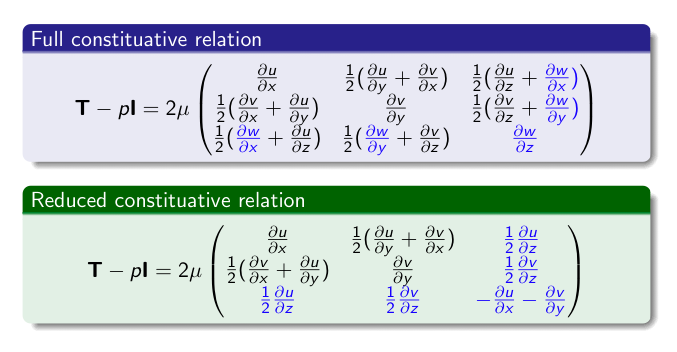
\includegraphics[width=0.7\columnwidth]{\dir/figs/HOeqns.eps}
   \end{center}
  \caption{Stokes-flow (top) and first-order (bottom) constitutive equations.}
  \label{fig:hoeqns}
\end{figure} 

\subsection{Available schemes}

\begin{itemize}
\item The most basic and fundamental higher-order scheme is the full, non-linear Stokes equations. Because of the computational burden, many 3d, large-scale models solve lower-order approximations to the Stokes equations (Figure \ref{fig:phylogeny}). However, a number of groups are making significant advances in this area and it seems likely that 3d, nonlinear-Stokes ice sheet models being used in climate-model applications is not far away (e.g. see the ELMER-Ice effort; \citet{gagliardini:2013iv}). Upcoming DOE-funded efforts will focus on implementing a nonlinear Stokes model on unstructured grids in CISM \citep{Leng:2012ia}.
\end{itemize}

\begin{itemize}
\item Probably the most long-lived higher-order approximation in glaciology is the shallow-shelf approxmation (or SSA) describing flow within an ice shelf (or ice stream if non-zero basal drag is included). It was made popular by Doug MacAyeal in the 80's and 90's (e.g., \citet{Macayeal:1989uo}). It's main disadvantage is that it is not fully 3d, as it assumes uniform velocity throughout the ice thickness driven only by horizontal stress gradients. It is, however, adequate for describing fast flow in many parts of the ice sheets, such as on ice shelves and along some ice streams. In this case, not resolving vertical gradients is a computational advantage.   
\end{itemize}

\begin{itemize}
\item The SSA equations are actually a depth-averaged form of a more general higher-order model, which is commonly referred to as the ``Blatter-Pattyn model" (\citet{BLATTER:1995wz}; \citet{Pattyn:2003tj}). This model has been around since the mid 90's and has become increasingly popular ever since. Blatter-Pattyn dynamics, synonymous with and more formally described as the ``first-order accurate Stokes approximation"\footnote{See \citet{Schoof:2010dl} and \citet{DUKOWICZ:2010wb} for a more complete scaling analysis and derivation of the first-order Stokes approximation.}, are currently implemented as the default higher-order dynamical core within CISM. 
\end{itemize}

\begin{itemize}
\item Several hybrid schemes exist that are computationally cheaper than the Blatter-Pattyn model. These combine solutions to the shallow ice approximation (for resolving vertical gradients) and the SSA approximation (for resolving horizontal gradients) in some clever way so that a fully 3d solution is obtained. It isn't yet known how well these model solutions compare to fully 3d models, or if one approach (hybrid vs. fully 3d solution) is superior to the other. David Pollard of Penn State and Ed Bueler of Univ. of Alaska Fairbanks currently run large-scale implementations of this type of model (\citet{Bueler:2009ee}; \citet{Pollard:2009ed}).
\end{itemize}

A good review paper that goes into a fair amount of detail about the various ice flow modeling approximations, their derivations, and their applicability, is the recent review by \citet{Schoof:2013is}.

\subsection{Practical differences between shallow ice models and higher-order models}

\begin{figure}
  \begin{center}
    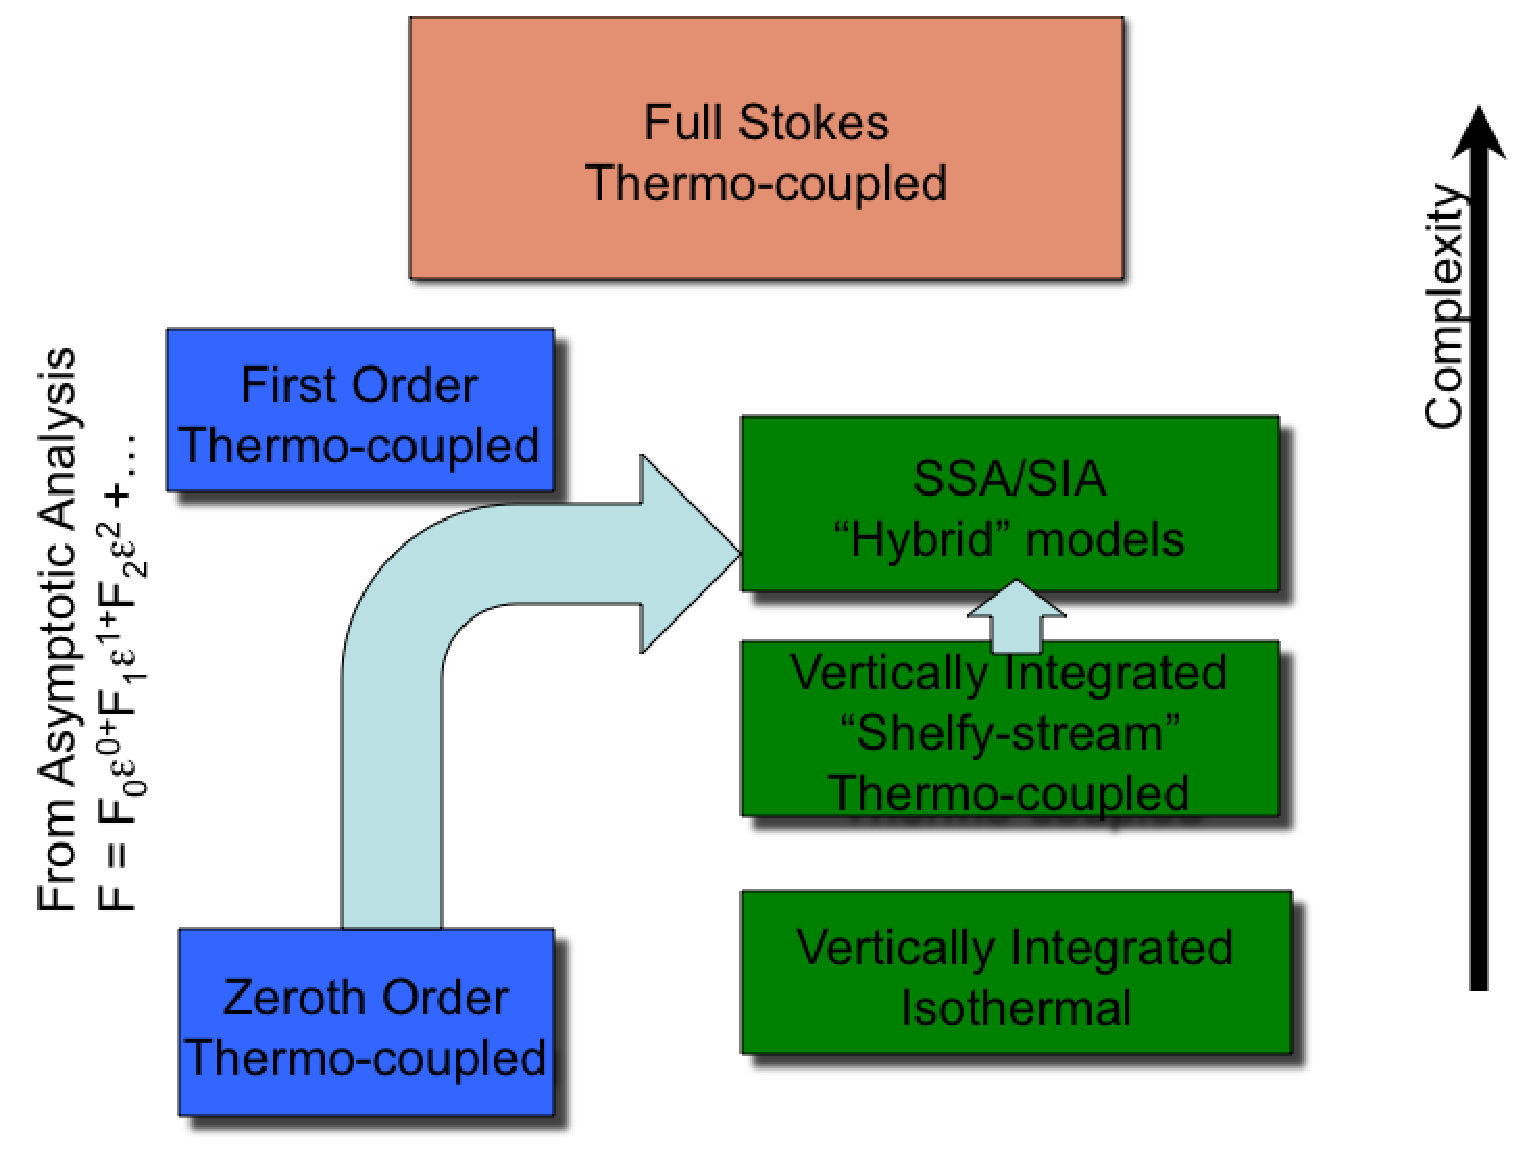
\includegraphics[width=0.5\columnwidth]{\dir/figs/ISMPhylogeny.eps}
   \end{center}
  \caption{The relationship between several common varieties of ice sheet modesl. Complexity increases along the vertical axis.}
   \label{fig:phylogeny}
\end{figure} 

By practical differences, we mean \textbf{(1)} how do we deal with solving the momentum equations in each case (the dynamics, or stress balance) and \textbf{(2)} how do we use the relevant information we derive from that solution (the kinematics, or velocity fields) to evolve the ice sheet geometry in time? There are large differences in how both of these issues are handled -- in shallow ice models versus in higher-order models -- for two main reasons:

\begin{itemize}
\item  The numerical solution of the dynamical equations is fundamentally different in each case. For the shallow ice case, we need only local information (slope and thickness) to solve for the velocity as a function of depth in a single column of ice. We do this pointwise for every location on our model domain (in map view), which is a relatively easy numerical problem; each column of velocities leads to a banded coefficient matrix that is relatively easy to invert (to solve for the velocities). This problem is also what we might call $embarrassingly$ $parallel$; in theory, each column of unknown velocities results in its own tridiagonal matrix, which could be solved for on its own processor. For higher-order models, however, we cannot do this since the solution at any point also depends on the solution at neighboring points (in map plane). The velocity at any point depends on non-local information, leading to an elliptic system of equations, and every velocity must be solved for simultaneously with every other velocity. The result is a much larger system of equations to solve, which is a more difficult numerical problem to solve on one processor and a much more difficult problem to solve on multiple processors. Because large-scale applications of higher-order models (e.g. whole-ice sheet models and coupling with climate models) will require efficient solution and parallelization techniques, this is a very active area of current research.  
\end{itemize}

\begin{itemize}
\item  The equations governing dynamics AND evolution in a shallow ice model can be recast together as a single, non-linear, diffusion equation for ice thickness. A single system of equations is solved to calculate the velocity field and evolve the ice sheet geometry. For higher-order models, we must first solve the momentum balance equations to obtain the velocity field. Then, we need to use some other scheme to evolve the ice thickness. 
\end{itemize}

Both of these differences mean that a model based on shallow ice physics may be built in a fundamentally different way than one based on higher-order physics. Most of the development work on CISM during the past few years has had to do with upgrading the model so that it can be used effectively and efficiently with higher-order dynamics schemes.  

The equations describing a (2d) higher-order flow that is vertically integrated (i.e., the SSA) are:

\begin{align*}
\frac{\partial}{\partial x}\left ( 2 \eta H 
\left(2\frac{\partial u}{\partial x}+\frac{\partial v}{\partial y}\right)\right)
+\frac{\partial}{\partial y}\left(\eta H\left(
\frac{\partial u}{\partial y}+\frac{\partial v}{\partial x}\right)\right)
=\rho_w gH \frac{\partial s}{\partial x}
\end{align*}


\begin{align*}
\frac{\partial}{\partial y}\left ( 2 \eta H 
\left(2\frac{\partial v}{\partial y}+\frac{\partial u}{\partial x}\right)\right)
+\frac{\partial}{\partial x}\left(\eta H\left(
\frac{\partial u}{\partial y}+\frac{\partial v}{\partial x}\right)\right)
=\rho_w gH \frac{\partial s}{\partial y}
\end{align*}

The equations describing a (3d) higher-order flow that is NOT vertically integrated (Blatter-Pattyn) are:

\begin{align*}
\frac{\partial}{\partial x}\left ( 2 \eta  
\left(2\frac{\partial u}{\partial x}+\frac{\partial v}{\partial y}\right)\right)
+\frac{\partial}{\partial y}\left(\eta \left(
\frac{\partial u}{\partial y}+\frac{\partial v}{\partial x}\right)\right)
+\frac{\partial}{\partial z}\left(\eta \frac{\partial u}{\partial z}\right)
=\rho_w g \frac{\partial s}{\partial x}
\end{align*}


\begin{align*}
\frac{\partial}{\partial y}\left ( 2 \eta 
\left(2\frac{\partial v}{\partial y}+\frac{\partial u}{\partial x}\right)\right)
+\frac{\partial}{\partial x}\left(\eta \left(
\frac{\partial u}{\partial y}+\frac{\partial v}{\partial x}\right)\right)
+\frac{\partial}{\partial z}\left(\eta \frac{\partial v}{\partial z}\right)
=\rho_w g \frac{\partial s}{\partial y}
\end{align*}

There are three differences that you should note
\begin{enumerate}
\item  The vertically integrated model includes the ice thickness, $H$, in each term. This is a reflection of the integration and does not appear in the first order equations.
\item  Accounting for the thickness not appearing, the only other difference is the presence of a vertical diffusion of horizontal velocities. This is the the third term on the left in the above equations.
\item  The first order equations must be solved on each of a set of horizontal layers. Layers communicate with each other through the vertical diffusion term.
\end{enumerate}

Both sets of equations are non-linear elliptical equations and much of the same technology can be used solve them. Additional complications come in when we account for boundary conditions at the lateral margins of the domain and at the upper and lower surfaces of the flow (note that for the vertically integrated flow, there are no explicit boundary conditions for the upper and lower surfaces; they are accounted for and incorporated during the vertical integration).

\subsection{Higher-order CISM}

\begin{figure}
  \begin{center}
    
\includegraphics[width=0.65\columnwidth]{\dir/figs/GIS.eps}
   \end{center}
  \caption{Observation-based balance velocities for Greenland (left) and depth-averaged speed from higher-order CISM (right) with basal sliding coefficients optimized to match the balance velocities (after Price et al., $PNAS$, \textbf{108}(22), 2011).}
  \label{fig:GIS_PNAS}
\end{figure} 

The higher-order dynamics scheme currently implemented in CISM (some output from which is shown in Figure \ref{fig:GIS_PNAS}) is discussed in more detail in the following chapters. First, the derivation of the equations themselves is discussed, followed by a discussion of the boundary conditions. Solutions methods for the nonlinear system of equations are then discussed. Finally, there is a brief discussion on the solution of the thickness evolution equation. 

A very useful higher-order model intercomparison project (ISMIP-HOM) was organized by Frank Pattyn from the Université Libre de Bruxelles. That project, which resulted in a set of "benchmark" experiments for higher-order models, is reported on formally in Pattyn et al. (2008). 

%\section{References}
%\begin{itemize}
%\item  \href{http://www.agu.org/journals/jf/jf0903/2008JF001179/}{Bueler, E. and J. Brown. Shallow shelf approximation as a "sliding law" in a thermomechanically coupled ice sheet model. \textit{J. Geophys. Res.}, F03008, doi:10.1029/2008JF001179, 2009.} 
%\item  \href{http://www.nature.com/nature/journal/v458/n7236/full/nature07809.html}{Pollard, D. and R.M. DeConto. Modelling West Antarctic ice sheet growth and collapse through the past five million years. \textit{Nature}, \textbf{458}, doi:10.1038/nature07809, 2009.}
%\item  \href{http://www.agu.org/journals/jb/jb0308/2002JB002329/}{Pattyn, F. A new three-dimensional higher-order thermomechanical ice sheet model: Basic sensitivity, ice stream development, and ice flow across subglacial lakes, \textit{J. Geophys. Res.}, \textbf{108}(B8), 2003.}
%\item  {Pattyn, F. and 20 others. Benchmark experiments for higher-order and full Stokes ice sheet models (ISMIP-HOM), \textit{The Cryosphere}, \textbf{2}, 2008.}
%\end{itemize}
%\end{document}

\section{Higher-Order Momentum Balance}
\label{sc:higher-order-mom}

\begin{figure}
  \begin{center}
    
\includegraphics[width=0.65\columnwidth]{\dir/figs/GIS.eps}
   \end{center}
  \caption{Observation-based balance velocities for Greenland (left) and depth-averaged speed from higher-order CISM (right) with basal sliding coefficients optimized to match the balance velocities (after Price et al., $PNAS$, \textbf{108}(22), 2011).}
  \label{fig:GIS_PNAS}
\end{figure} 

The higher-order dynamics scheme in CISM (some output from which is shown in Figure \ref{fig:GIS_PNAS}) is discussed in more detail in the following sections. 
First we describe the derivation of the equations themselves, followed by a discussion and derivation of the boundary conditions.
We then describe generic solution methods for the nonlinear system of equations, followed by a
brief discussion of the solution of the thickness evolution equation.

% Commented out the subsection because there are no other subsections in this section
%\subsection{Derivation of the Blatter-Pattyn Equations}
%\label{sc:higher-order-blatter-pattyn}

The higher-order dynamics scheme in CISM is based on the 3d first-order accurate Stokes approximation (also often referred to as the ``Blatter-Pattyn" model). The starting point is the nonlinear Stokes equations:

\begin{equation}
  \begin{split}
    & x:\quad \frac{\partial \tau _{xx}}{\partial x} + \frac{\partial \tau _{xy}}{\partial y} + \frac{\partial \tau _{xz}}{\partial z} - \frac{\partial P}{\partial x} = 0, \\ 
    & y:\quad \frac{\partial \tau _{xy}}{\partial x} + \frac{\partial \tau _{yy}}{\partial y} + \frac{\partial \tau _{yz}}{\partial z} - \frac{\partial P}{\partial y} = 0, \\ 
    & z:\quad \frac{\partial \tau _{xz}}{\partial x} + \frac{\partial \tau _{zy}}{\partial y} + \frac{\partial \tau _{zz}}{\partial z} - \frac{\partial P}{\partial z} = \rho_i g,
  \end{split}
\end{equation}

\noindent
where \textit{P} is the pressure and {\large \(\tau{}\)} is the deviatoric stress tensor. The latter is given by $\tau _{ij}=\sigma _{ij}+P\delta _{ij}$, 
where {\large \(\sigma{}\)} is the full stress tensor.

There are a number of ways to argue that, due to the shallowness of ice sheets (i.e., the small value of \textit{H}/\textit{L}, where \textit{H} is the thickness and \textit{L} is a relevant horizontal length scale), the Stokes equations can be reduced to the following first-order approximation:

\begin{equation}
  \begin{split}
    & x:\quad \frac{\partial \tau _{xx}}{\partial x} + \frac{\partial \tau _{xy}}{\partial y} + \frac{\partial \tau _{xz}}{\partial z} - \frac{\partial P}{\partial x} = 0, \\ 
    & y:\quad \frac{\partial \tau _{yy}}{\partial y} + \frac{\partial \tau _{xy}}{\partial x} + \frac{\partial \tau _{yz}}{\partial z} - \frac{\partial P}{\partial y} = 0, \\ 
    & z:\quad \frac{\partial \tau _{zz}}{\partial z} - \frac{\partial P}{\partial z} = \rho g. \\ 
  \end{split}
\end{equation}

\noindent
The arguments supporting this reduction are fairly complex and are based on either a variational analysis or an asymptotic analysis (see \citet{Schoof:2010dl} and \citet{DUKOWICZ:2010wb} for details).

The third (vertical) balance equation above can be integrated vertically to give an expression for the pressure:
\begin{equation}
P = \rho g\left( s-z \right) + \tau _{zz}(z).
\end{equation} 
This is simply a statement that the full vertical normal stress is balanced by the hydrostatic pressure (the so-called \textit{hydrostatic assumption}). This expression can be substituted into the horizontal pressure gradient terms above to remove pressure from the equations. For example, for the \textit{x} component of velocity we have

\begin{equation}
  \label{ho.eq.x_stress_balance}
  \begin{split}
    & \frac{\partial \tau _{xx}}{\partial x} + \frac{\partial \tau _{xy}}{\partial y} + \frac{\partial \tau _{xz}}{\partial z} = \frac{\partial }{\partial x}\left[ \rho g\left( s-z \right)+\tau _{zz}(z) \right] \\ 
    & \frac{\partial \tau _{xx}}{\partial x} - \frac{\partial \tau _{zz}}{\partial x} + \frac{\partial \tau _{xy}}{\partial y} + \frac{\partial \tau _{xz}}{\partial z} = \rho g\frac{\partial s}{\partial x} \\ 
  \end{split}
\end{equation}

\noindent
Using the incompressibility constraint \eqref{ho.eq.incompress} and the assumption that stress and strain are aligned we can write

\begin{equation}
  \label{ho.eq.incompress_tau}
  \tau _{zz} = -\tau _{xx}-\tau _{yy}.
\end{equation}

\noindent
Taking the gradient of \eqref{ho.eq.incompress_tau} with respect to $x$, we can rewrite the vertical normal deviatoric stress in terms of horizontal normal deviatoric stresses:

\begin{equation}
  \label{ho.eq.incompress_tau_dx}
  -\frac{\partial \tau _{zz}}{\partial x} = -\frac{\partial }{\partial x}\left( -\tau _{xx} - \tau _{yy} \right) = \frac{\partial \tau _{xx}}{\partial x} + \frac{\partial \tau _{yy}}{\partial x}.
\end{equation}
 
\noindent
Substituting \eqref{ho.eq.incompress_tau_dx} into \eqref{ho.eq.x_stress_balance}, we obtain
 
\begin{equation}
%  2\frac{\partial \tau _{xx}}{\partial x} + \frac{\partial \tau _{yy}}{\partial x} + \frac{\partial \tau _{xy}}{\partial y} + \frac{\partial \tau _{xz}}{\partial z} = \rho g\frac{\partial s}{\partial x}.
  \label{ho.eq.stress_balance_x}
  \frac{\partial }{\partial x} \left( 2 \tau_{xx} + \tau_{yy} \right) + \frac{\partial \tau _{xy}}{\partial y} + \frac{\partial \tau _{xz}}{\partial z} = \rho g\frac{\partial s}{\partial x}.
\end{equation}

\noindent
Similarly, the $y$ horizontal balance equation is
\begin{equation}
  \label{ho.eq.stress_balance_y}
  \frac{\partial }{\partial y} \left( 2 \tau_{yy} + \tau_{xx} \right) + \frac{\partial \tau _{xy}}{\partial x} + \frac{\partial \tau _{yz}}{\partial z} = \rho g\frac{\partial s}{\partial y}.
\end{equation}

\noindent 
At this point we have removed the vertical balance equation entirely; it has been incorporated into the horizontal balance equations through incompressibility.


%\begin{align*}
%  & x:\quad 2\frac{\partial \tau _{xx}}{\partial x}+\frac{\partial \tau _{yy}}{\partial x}+\frac{\partial \tau _{xy}}{\partial y}+\frac{\partial \tau _{xz}}{\partial z}=\rho g\frac{\partial s}{\partial x}\quad,  \\ 
% & y:\quad 2\frac{\partial \tau _{yy}}{\partial y}+\frac{\partial \tau _{xx}}{\partial y}+\frac{\partial \tau _{xy}}{\partial x}+\frac{\partial \tau _{yz}}{\partial z}=\rho g\frac{\partial s}{\partial y}. \\
%\end{align*}

Next we want to write these equations in terms of the velocities for which we are ultimately solving. Stresses and velocities are linked through the 
constitutive law for ice, which relates strain rates to stresses (here we assume Nye's generalization of Glen's law), and through the 
definition of the strain rate tensor, which relates strain rates to velocity gradients:

\begin{equation}
  \begin{split}
    & 1.\quad \tau _{ij}=B\dot{\varepsilon }_{e}^{\frac{1-n}{n}}\dot{\varepsilon }_{ij},\quad B=B(T) \\ 
    & 2.\quad \dot{\varepsilon }_{ij}=\frac{1}{2}\left( \frac{\partial u_{i}}{\partial x_{j}}+\frac{\partial u_{j}}{\partial x_{i}} \right) \\ 
    & 3.\quad 2\dot{\varepsilon }_{e}=\dot{\varepsilon }_{ij}\dot{\varepsilon }_{ij} \\ 
    & 4.\quad \eta \equiv \frac{1}{2}B\dot{\varepsilon }_{e}^{\frac{1-n}{n}} \\ 
    & 5.\quad \tau _{ij}=2\eta \dot{\varepsilon }_{ij} \\ 
  \end{split}
\end{equation}

\noindent
In order, the five expressions above give: 

\begin{enumerate}
\item  Glen's flow law\footnote{Technically, we are using the \textit{inverse} form of the flow-law here.}, where 
$B = A^{\frac{-1}{n}}$ is the temperature dependent rate factor 
\item  The definition of the strain-rate tensor in terms of velocity gradients
\item  The definition of the effective strain rate, $\dot{\varepsilon }_{e}$, a norm of the strain-rate tensor
\item  A definition of the ``effective viscosity" (after rearranging some terms in (1))
\item  Items (1)-(4) allow us to write the relationship between stress and strain in a standard ``Newtonian" way, but with a non-Newtonian (nonlinear) viscosity
\end{enumerate}

\noindent
Now, taking these definitions into the stress balance equations \eqref{ho.eq.stress_balance_x} and \eqref{ho.eq.stress_balance_y} 
and expanding in terms of strain rates and effective viscosity, we have (for the \textit{x} direction only):

\begin{equation}
  x: \quad 2\frac{\partial }{\partial x}\left( 2\eta \dot{\varepsilon }_{xx} \right) + \frac{\partial }{\partial x}\left( 2\eta \dot{\varepsilon }_{yy
} \right) + \frac{\partial }{\partial y}\left( 2\eta \dot{\varepsilon }_{xy} \right) + \frac{\partial }{\partial z}\left( 2\eta \dot{\varepsilon }_{xz} 
\right) = \rho g\frac{\partial s}{\partial x}, \\ 
%  x: \quad 2\frac{\partial }{\partial x} \left( 2\eta \dot{\varepsilon }_{xx} +  2\eta \dot{\varepsilon}_{yy} \right) +\frac{\partial }{\partial y}\left( 2\eta \dot{\varepsilon }_{xy} \right)+\frac{\partial }{\partial z}\left( 2\eta \dot{\varepsilon }_{xz} \right)=\rho g\frac{\partial s}{\partial x}. \\ 
\end{equation}

\noindent
Replacing strain-rate components with velocity gradients, we obtain

\begin{equation}
  \label{ho.eq.stress_balance_final_x}
  x: \quad \frac{\partial }{\partial x}\left( 4 \eta \frac{\partial u}{\partial x} +  2 \eta \frac{\partial v}{\partial y} \right) + \frac{\partial }{\partial y}\left[ \eta \left( \frac{\partial u}{\partial y} + \frac{\partial v}{\partial x} \right) \right]+\frac{\partial }{\partial z}\left( \eta \frac{\partial u}{\partial z} \right) = \rho g\frac{\partial s}{\partial x}.
\end{equation}

\noindent
An analogous expression gives the \textit{y}-direction momentum balance: 

\begin{equation}
  \label{ho.eq.stress_balance_final_y}
  y: \quad \frac{\partial }{\partial y}\left( 4 \eta \frac{\partial v}{\partial y} +  2 \eta \frac{\partial u}{\partial x} \right) + \frac{\partial }{\partial x}\left[ \eta \left( \frac{\partial u}{\partial y} + \frac{\partial v}{\partial x} \right) \right]+\frac{\partial }{\partial z}\left( \eta \frac{\partial v}{\partial z} \right) = \rho g\frac{\partial s}{\partial y}.  
\end{equation}

\noindent
These are the basic equations to be discretized and solved.

%Thus, the final form of the equations to be discretized and solved is given by:

%\begin{align*}
%  & x:\quad 4\frac{\partial }{\partial x}\left( \eta \frac{\partial u}{\partial x} \right)+\frac{\partial }{\partial y}\left( \eta \frac{\partial u}{\partial y} \right)
%  +2\frac{\partial }{\partial x}\left( \eta \frac{\partial v}{\partial y} \right)+\frac{\partial }{\partial y}\left( \eta \frac{\partial v}{\partial x} \right)
%  +\frac{\partial }{\partial z}\left( \eta \frac{\partial u}{\partial z} \right)=\rho g\frac{\partial s}{\partial x}, \\ 
% & y:\quad 4\frac{\partial }{\partial y}\left( \eta \frac{\partial v}{\partial y} \right)+\frac{\partial }{\partial x}\left( \eta \frac{\partial v}{\partial x} \right)
% +2\frac{\partial }{\partial y}\left( \eta \frac{\partial u}{\partial x} \right)+\frac{\partial }{\partial x}\left( \eta \frac{\partial u}{\partial y} \right)
% +\frac{\partial }{\partial z}\left( \eta \frac{\partial v}{\partial z} \right)=\rho g\frac{\partial s}{\partial y}. \\ 
%\end{align*}


\section{Higher-Order Model Boundary Conditions}
\label{sc:higher-order-bcs}

We now carry out an approximate derivation of the boundary conditions that are implemented with CISM's higher-order scheme. By approximate we mean that some of the derivation is guided by physical intuition and reasonable arguments, rather than rigorous mathematics. In the end, we derive the same set of equations as when following the more rigorous approach (see, e.g. \citet{DUKOWICZ:2010wb}). We will look at the derivation in three parts, (1) the free surface boundary condition, (2) the basal traction boundary condition, and (3) lateral boundary conditions.

\subsection{Stress-free Surface}
At the upper ice surface, a stress-free boundary condition is applied. The traction vector $T_i$ must be continuous across the ice sheet surface and, assuming that atmospheric pressure and surface tension are small, we have

\begin{equation}
  \label{ho.eq.surface_traction}
  \begin{split}
    & T_{i} = -T_{i(\textrm{boundary})}\approx 0, \\ 
    & T_{i} = \sigma _{ij}n_{j} = \sigma _{i1}n_{1} + \sigma _{i2}n_{2} + \sigma _{i3}n_{3} = 0, \\
  \end{split}
\end{equation}

\noindent
where the $n_i$ are the components of the outward facing, unit normal vector in Cartesian coordinates.

For a function \textit{F(x,y,z) = z -- f(x,y) = 0}, where \textit{z = f(x,y)} defines the surface, the gradient of \textit{F(x,y,z)} gives the components of the surface normal vector. For the case of the ice sheet surface, $s = f(x,y)$ and the surface normal is given by

\begin{equation}
  n_{i}=\left( -\frac{\partial s}{\partial x},-\frac{\partial s}{\partial y},1 \right)\frac{1}{a},
\end{equation}

\noindent
where

\begin{equation}
  a = \sqrt{\left( \frac{\partial s}{\partial x} \right)^{2} + \left( \frac{\partial s}{\partial y} \right)^{2} + 1}.
\end{equation}

\noindent
Eq. \eqref{ho.eq.surface_traction} gives three equations that must be satisfied at the free surface:

\begin{equation}
  \begin{split}
    & i=x: \quad T_{x} = \sigma _{xx}n_{x} + \sigma _{xy}n_{y} + \sigma _{xz}n_{z}=0, \\ 
    & i=y: \quad T_{y} = \sigma _{yx}n_{x} + \sigma _{yy}n_{y} + \sigma _{yz}n_{z}=0, \\ 
    & i=z: \quad T_{z} = \sigma _{zx}n_{x} + \sigma _{zy}n_{y} + \sigma _{zz}n_{z}=0. \\ 
  \end{split}
\end{equation}

\noindent
Expanding the $z$ equation and expressing stresses in terms of strain rates and pressures, where $\eta$ is the effective viscosity defined above, gives

\begin{equation}
  \left( 2\eta \dot{\varepsilon }_{zx} \right)n_{x}+\left( 2\eta \dot{\varepsilon }_{zy} \right)n_{y}+\left( 2\eta \dot{\varepsilon }_{zz}-P \right)n_{z}=0.
\end{equation}

\noindent
Solving for the pressure gives

\begin{equation}
  Pn_{z} = \left( 2\eta \dot{\varepsilon }_{zz} \right)n_{z}+\left( 2\eta \dot{\varepsilon }_{zx} \right)n_{x}+\left( 2\eta \dot{\varepsilon }_{zy} \right)n_{y}.
\end{equation}

\noindent
Expanding in terms of velocity gradients and normal vector components, we find

\begin{equation}
  P = 2\eta \frac{\partial w}{\partial z}-\left( \eta \frac{\partial u}{\partial z} \right)\frac{\partial s}{\partial x}-\left( \eta \frac{\partial v}{\partial z} \right)\frac{\partial s}{\partial y},
\end{equation}

where we have made the usual first-order approximation that 

\begin{equation}
  \frac{\partial w}{\partial x}=\frac{\partial w}{\partial y}\approx 0.
\end{equation}

\noindent
\textit{(WHL: and also assumed $a \approx 1$?)}

\textbf{WHL: The rest of this section derives BC discretizations that were used in Glam but are not necessary
in a finite-element approach. So I think the remaining text could be rewritten a bit and considerably shortened.}

We use this expression for the pressure and expand the two horizontal boundary condition expressions

\begin{equation}
\begin{split}
 & i=x:\quad T_{x}=\sigma _{xx}n_{x}+\sigma _{xy}n_{y}+\sigma _{xz}n_{z}=0, \\ 
 & i=y:\quad T_{y}=\sigma _{yx}n_{x}+\sigma _{yy}n_{y}+\sigma _{yz}n_{z}=0, \\
\end{split}
 \end{equation}

in terms of velocity gradients and the effective viscosity to obtain

\begin{equation}
\begin{split}
   {} & \hat{x}:\quad -2\eta \frac{\partial u}{\partial x}\frac{\partial s}{\partial x}-\eta \left( \frac{\partial u}{\partial y}+\frac{\partial v}{\partial x} \right)\frac{\partial s}{\partial y}+\eta \frac{\partial u}{\partial z}=  \\
   {} & \quad \quad \quad \quad \quad -2\eta \frac{\partial w}{\partial z}\frac{\partial s}{\partial x}+\eta \frac{\partial u}{\partial z}\left[ \frac{\partial s}{\partial x}\frac{\partial s}{\partial x} \right]+\eta \frac{\partial v}{\partial z}\left[ \frac{\partial s}{\partial y}\frac{\partial s}{\partial x} \right],  \\
%\end{equation}
%
%\begin{equation}
   {} & \hat{y}:\quad -2\eta \frac{\partial v}{\partial y}\frac{\partial s}{\partial y}-\eta \left( \frac{\partial u}{\partial y}+\frac{\partial v}{\partial x} \right)\frac{\partial s}{\partial x}+\eta \frac{\partial v}{\partial z}=  \\
   {} & \quad \quad \quad \quad \quad -2\eta \frac{\partial w}{\partial z}\frac{\partial s}{\partial y}+\eta \frac{\partial u}{\partial z}\left[ \frac{\partial s}{\partial x}\frac{\partial s}{\partial y} \right]+\eta \frac{\partial v}{\partial z}\left[ \frac{\partial s}{\partial y}\frac{\partial s}{\partial y} \right].  \\
\end{split}
\end{equation}

In both of these expression, the terms in square brackets are $\sim{0}$ (because slopes on ice sheets are small and the slope squared is exceedingly small). From continuity, we also have

\begin{equation}
\frac{\partial w}{\partial z}=-\frac{\partial u}{\partial x}-\frac{\partial v}{\partial y}.
\end{equation}

Using this expression for the normal vertical velocity gradient and removing the terms in square brackets our two horizontal boundary condition expressions become

\begin{equation}
\begin{split}
   {} & \hat{x}:\quad -2\eta \frac{\partial u}{\partial x}\frac{\partial s}{\partial x}-\eta \left( \frac{\partial u}{\partial y}+\frac{\partial v}{\partial x} \right)\frac{\partial s}{\partial y}+\eta \frac{\partial u}{\partial z}=2\eta \left( \frac{\partial u}{\partial x}\frac{\partial s}{\partial x}+\frac{\partial v}{\partial y}\frac{\partial s}{\partial x} \right),  \\
   {} & \hat{y}:\quad -2\eta \frac{\partial v}{\partial y}\frac{\partial s}{\partial y}-\eta \left( \frac{\partial u}{\partial y}+\frac{\partial v}{\partial x} \right)\frac{\partial s}{\partial x}+\eta \frac{\partial v}{\partial z}=2\eta \left( \frac{\partial u}{\partial x}\frac{\partial s}{\partial y}+\frac{\partial v}{\partial y}\frac{\partial s}{\partial y} \right).  \\
\end{split}
\end{equation}

%As in the derivation of the 1st-order stress balance equations, collect terms of a particular velocity gradient (that is, \textit{u} or \textit{v}) and move them to one side of the equation 
Moving terms to one side and dividing through by the effective viscosity \textit{\(\eta{}\)}, we arrive at the final form of the 1st-order, free surface boundary conditions

\begin{equation}
\begin{split}
   {} & \hat{x}:\quad 4\frac{\partial u}{\partial x}\frac{\partial s}{\partial x}+\frac{\partial u}{\partial y}\frac{\partial s}{\partial y}+2\frac{\partial v}{\partial y}\frac{\partial s}{\partial x}+\frac{\partial v}{\partial x}\frac{\partial s}{\partial y}-\frac{\partial u}{\partial z}=0,  \\
   {} & \hat{y}:\quad 4\frac{\partial v}{\partial y}\frac{\partial s}{\partial y}+\frac{\partial v}{\partial x}\frac{\partial s}{\partial x}+2\frac{\partial u}{\partial x}\frac{\partial s}{\partial y}+\frac{\partial u}{\partial y}\frac{\partial s}{\partial x}-\frac{\partial v}{\partial z}=0.  \\
\end{split}
\end{equation}

\subsection{Specified Basal Traction}
Derivation of the basal boundary condition follows that above for the free surface except that,
\begin{enumerate}

\item the right-hand side of the equation is not zero, rather it consists of an assumed basal traction vector with components 
\begin{equation}
\tau_{bi} = \left( \tau _{bx},\tau _{by} \right),
\end{equation}

\item the outward facing normal vector components now consist of horizontal gradients in the basal surface (with a resulting sign switch on the $x,y,z$ components relative to the upper surface)

\item the effective viscosity does not disappear from the equations when we divide through
\end{enumerate}

Making these substitutions we obtain the 1st-order basal boundary conditions for a specified basal traction

\begin{equation}
\begin{split}
  & \hat{x}:\quad 4\frac{\partial u}{\partial x}\frac{\partial b}{\partial x}+\frac{\partial u}{\partial y}\frac{\partial b}{\partial y}+2\frac{\partial v}{\partial y}\frac{\partial b}{\partial x}+\frac{\partial v}{\partial x}\frac{\partial b}{\partial y}-\frac{\partial u}{\partial z}=\frac{\tau _{bx}}{\eta }, \\ 
 & \hat{y}:\quad 4\frac{\partial v}{\partial y}\frac{\partial b}{\partial y}+\frac{\partial v}{\partial x}\frac{\partial b}{\partial x}+2\frac{\partial u}{\partial x}\frac{\partial b}{\partial y}+\frac{\partial u}{\partial y}\frac{\partial b}{\partial x}-\frac{\partial v}{\partial z}=\frac{\tau _{by}}{\eta }. \\
\end{split}
 \end{equation}

We assume that basal traction is linearly related to basal sliding velocity through a positive traction parameter, $\beta$, such that

\begin{equation}
\label{basaltraction}
\tau _{bx}=\left. -\beta u \right|_{z=b},\quad \tau _{by}=\left. -\beta v \right|_{z=b}.
\end{equation}

Note that the negative sign in front of the $\beta$ indicates that the traction vector is oriented parallel to and in the opposite direction of the sliding velocity vector.

Substituting this expression into the above gives our final horizontal boundary conditions at the ice sheet base

\begin{equation}
\begin{split}
  & \hat{x}:\quad 4\frac{\partial u}{\partial x}\frac{\partial b}{\partial x}+\frac{\partial u}{\partial y}\frac{\partial b}{\partial y}+2\frac{\partial v}{\partial y}\frac{\partial b}{\partial x}+\frac{\partial v}{\partial x}\frac{\partial b}{\partial y}-\frac{\partial u}{\partial z}+\left( \frac{B}{\eta } \right)u=0, \\ 
 & \hat{y}:\quad 4\frac{\partial v}{\partial y}\frac{\partial b}{\partial y}+\frac{\partial v}{\partial x}\frac{\partial b}{\partial x}+2\frac{\partial u}{\partial x}\frac{\partial b}{\partial y}+\frac{\partial u}{\partial y}\frac{\partial b}{\partial x}-\frac{\partial v}{\partial z}+\left( \frac{B}{\eta } \right)v=0. \\
\end{split}
 \end{equation}

The use of a linear traction parameter (Eq. \ref{basaltraction}) can be modified to
implement basal friction laws that are a function of effective pressure 
(ice overburden pressure minus water pressure at the bed) and 
(generally) nonlinear in the sliding velocity.  Two such basal friction laws are
implemented in CISM.  For friction laws that are nonlinear in sliding velocity,
$\beta$ in eq. \ref{basaltraction} becomes a function of sliding velocity.  This is
implemented by lagging the value of sliding velocity used to calculate an ``effective'' 
$\beta$ in the fixed-point iterations used to solve the momentum balance.

The first is a Weertman-style friction law \citep{Weertman1957, Weertman1964} modified 
to include an effective pressure dependence \citep{Bindschadler1983, Budd1979}.
Notation here follows the summary by \citet[][p.240, eq.7.17]{Cuffey2010}.  The form of
the friction law is:
\begin{equation}
  \label{weertmansliding}
  \vec{u_b} = k \vec{\tau_{b}}^p N^{-q}
\end{equation}
which can be rearranged for $\vec{\tau_b}$ as:
\begin{equation}
  \label{weertmansliding2}
  \vec{\tau_b} = k^\frac{-1}{p} \vec{u_b}^\frac{1}{p} N^\frac{q}{p}
\end{equation}
where $k$ is a friction coefficient based on thermal and mechanical properties of ice 
and inversely related to bed roughness.  \citet{Cuffey2010} suggest values of 
$p=3$ and $q=1$, making this nonlinear in velocity.  

One problem with Eq. \ref{weertmansliding} is that it allows for unbounded basal traction.
An improvement to this is a physically-based basal friction law for sliding over 
hard beds that allows for cavitation and bounded basal drag \citep[]{Schoof2005}, 
the second friction law in CISM that accounts for effective pressure: 
\begin{equation}
    \label{CF-law}
	  \vec{\tau_b} = C \left( \frac{ \vec{u_b} } { \vec{u_b} + N^n \Lambda} \right)^{1/n} N,   \Lambda=\frac{\lambda_{max}A}{m_{max}}
\end{equation}
In Eq. \ref{CF-law}, $C$ is a Coulomb friction coefficient,  and $\lambda_{max}$ and 
$m_{max}$ are the wavelength (m) and maximum slope, respectively, of the 
dominant bedrock bumps.  Near cavitation (i.e., when effective pressure approaches 
0 at high water pressure), the friction law becomes a Coulomb friction law of the 
form $\vec{\tau_b}=CN$. Alternatively, at large effective pressures (low water pressure) 
the friction law takes a power law form, $\vec{\tau_b} \propto u_b^{1/n}$. 
The representation of bump geometry in the friction law is at a sub-grid scale 
and not explicitly resolved in the grid geometry used by the model.

[Note that the release version of CISM does not currently include a hydrology model
that outputs effective pressure, so at present effective pressure fields must be
input as data to use these two basal friction laws.]

\subsection{Specified Basal Yield Stress}
The above implementation of a specified basal traction can be altered to simulate sliding over a sediment-covered bed for which the sediment has a plastic or ``Coulomb friction" rheology. That is, sliding does not occur below the specified yield stress of the underlying material (e.g., a water saturated subglacial till). When the yield stress, $\tau_0$ is reached, sliding occurs at a rate that maintains but does not exceed that yield stress. Consider the \textit{x} direction boundary condition above, written out in terms of basal stress components,

\begin{equation}
\begin{split}
  & \hat{x}:\quad 4\eta \frac{\partial u}{\partial x}\frac{\partial b}{\partial x}+\eta \frac{\partial u}{\partial y}\frac{\partial b}{\partial y}+2\eta \frac{\partial v}{\partial y}\frac{\partial b}{\partial x}+\eta \frac{\partial v}{\partial x}\frac{\partial b}{\partial y}-\eta \frac{\partial u}{\partial z}=\tau _{bx}, \\ 
 & \quad \quad \quad \quad \quad \quad \tau _{bx}\approx \tau _{0}=\tau _{0}\left( \frac{u}{\left| \mathbf{u} \right|} \right)=\tau _{0}\left( \frac{u}{\sqrt{u_{0}^{2}+v_{0}^{2}+\gamma }} \right) \\ 
\end{split}
\end{equation}

In the expression above, $u$ is the $x$ component of the basal sliding velocity from the current iteration, $u_0$ and $v_0$ are components from the previous iteration, and $\gamma$ is a regularization constant (a small constant number to avoid division by zero during early iterations). Note that as the solution converges, velocities at the current and previous iteration are nearly equal, and the expression in parentheses approaches 1, in which case the basal stress and yield stress are approximately equal. 

We can accommodate this into our earlier framework for incorporating the traction parameter $\beta$ by treating $\beta$ as being nonlinear and dependent on the velocity,

\begin{equation}
\begin{split}
  & \tau _{bx}=-\beta u,\quad \quad  \\ 
 & \beta \equiv \frac{\tau _{0}}{\sqrt{u_{0}^{2}+v_{0}^{2}+\gamma }},\quad  \\ 
 & \tau _{bx}=-\left( \frac{\tau _{0}}{\sqrt{u_{0}^{2}+v_{0}^{2}+\gamma }} \right)u.\quad  \\
\end{split}
\end{equation}

Thus, we can implement plastic bed sliding behavior simply by substituting the above expression for our ``nonlinear" \textit{{\large \(\beta{}\)}} into our previous expressions for the basal boundary conditions in \textit{x} (a similar expression applies for the \textit{y} direction). 
%Figures \ref{fig:plasticbed1} and \ref{fig:plasticbed2} below show some examples of this type of boundary condition for the case of an idealized ice stream.
Figure \ref{fig:plasticbed1} shows an example of this type of boundary condition for the case of an idealized ice stream simulated by CISM.

\begin{figure}
  \begin{center}
    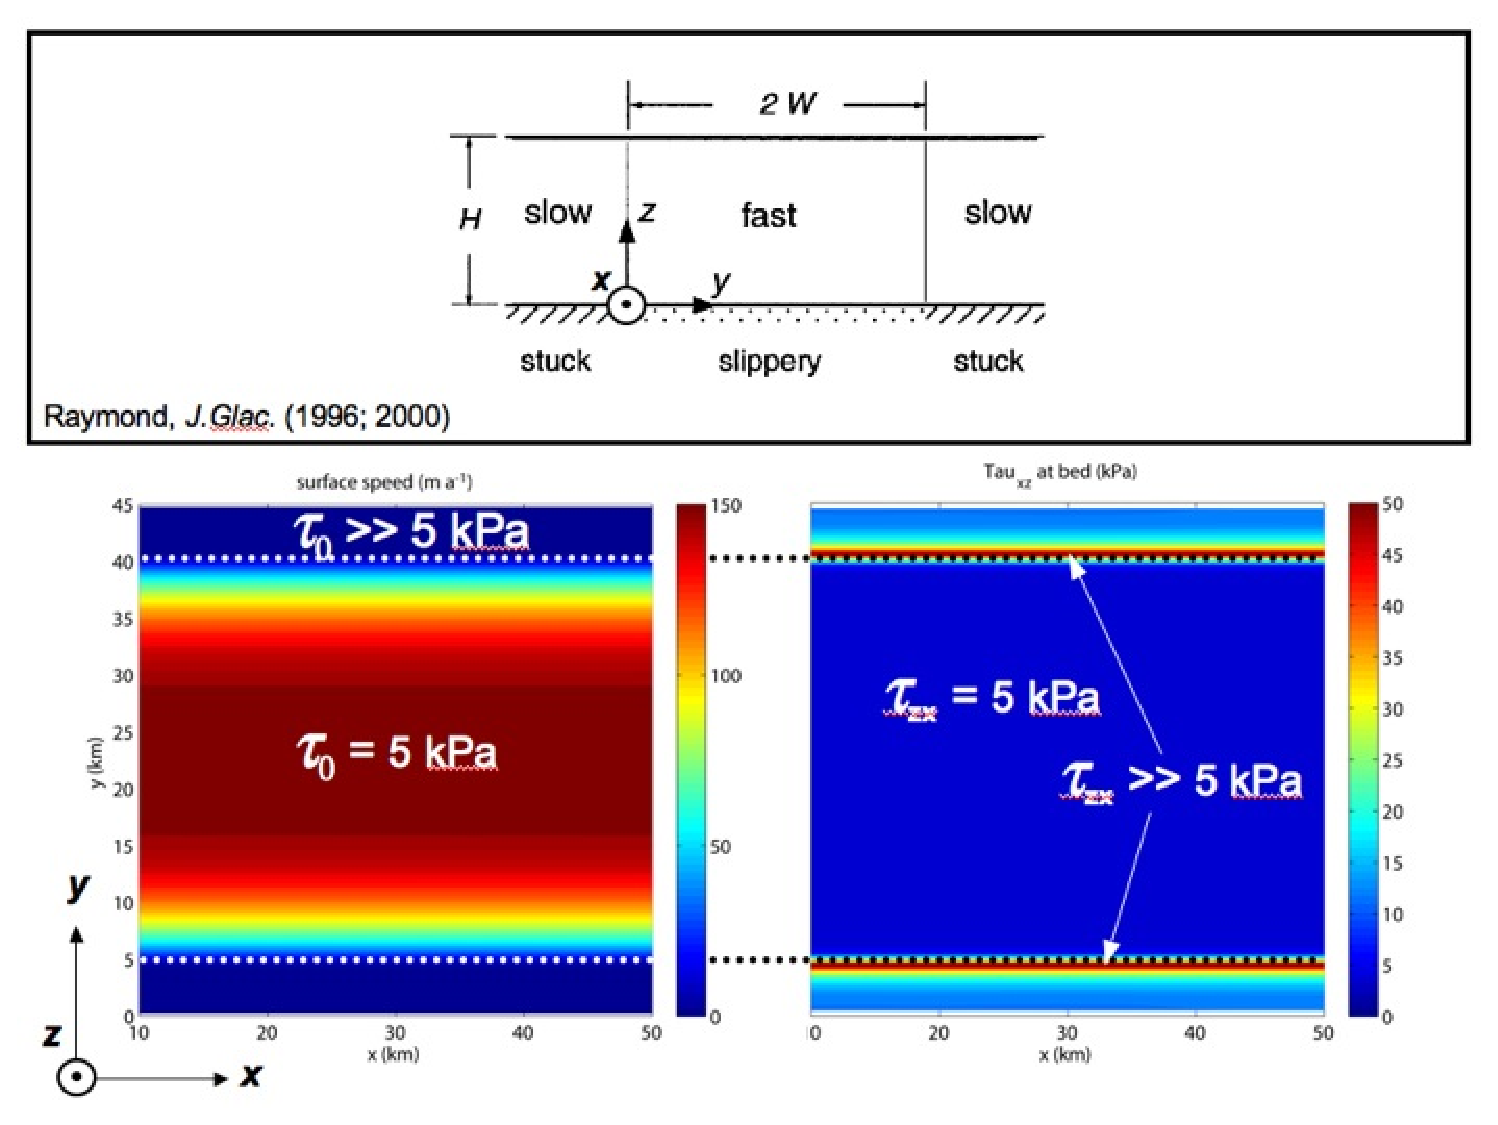
\includegraphics[width=0.65\columnwidth]{\dir/figs/Plastic_bed1.eps}
  \end{center}
  \caption{Idealized ice stream with plastic-bed sliding. Top panel shows a schematic of an idealized ice stream, frozen at the margins and thawed within the ice stream (flow is out of the page). Bottom panel (color) shows a modeled, idealized ice stream (flow is from left to right) with a yield stress of 5 kPa within the ice stream and much larger than 5 kPa outside of it. Bottom left shows the ice stream speed (m/yr) and the bottom right shows the basal drag (kPa). Within the ice stream basal drag is equal to the yield stress. Outside of the ice stream, stress transfer to the lateral margins results in basal drag that is much larger than the yield stress (and also much larger than the driving stress).}
  \label{fig:plasticbed1}
\end{figure} 

%\begin{figure}
%  \begin{center}
%    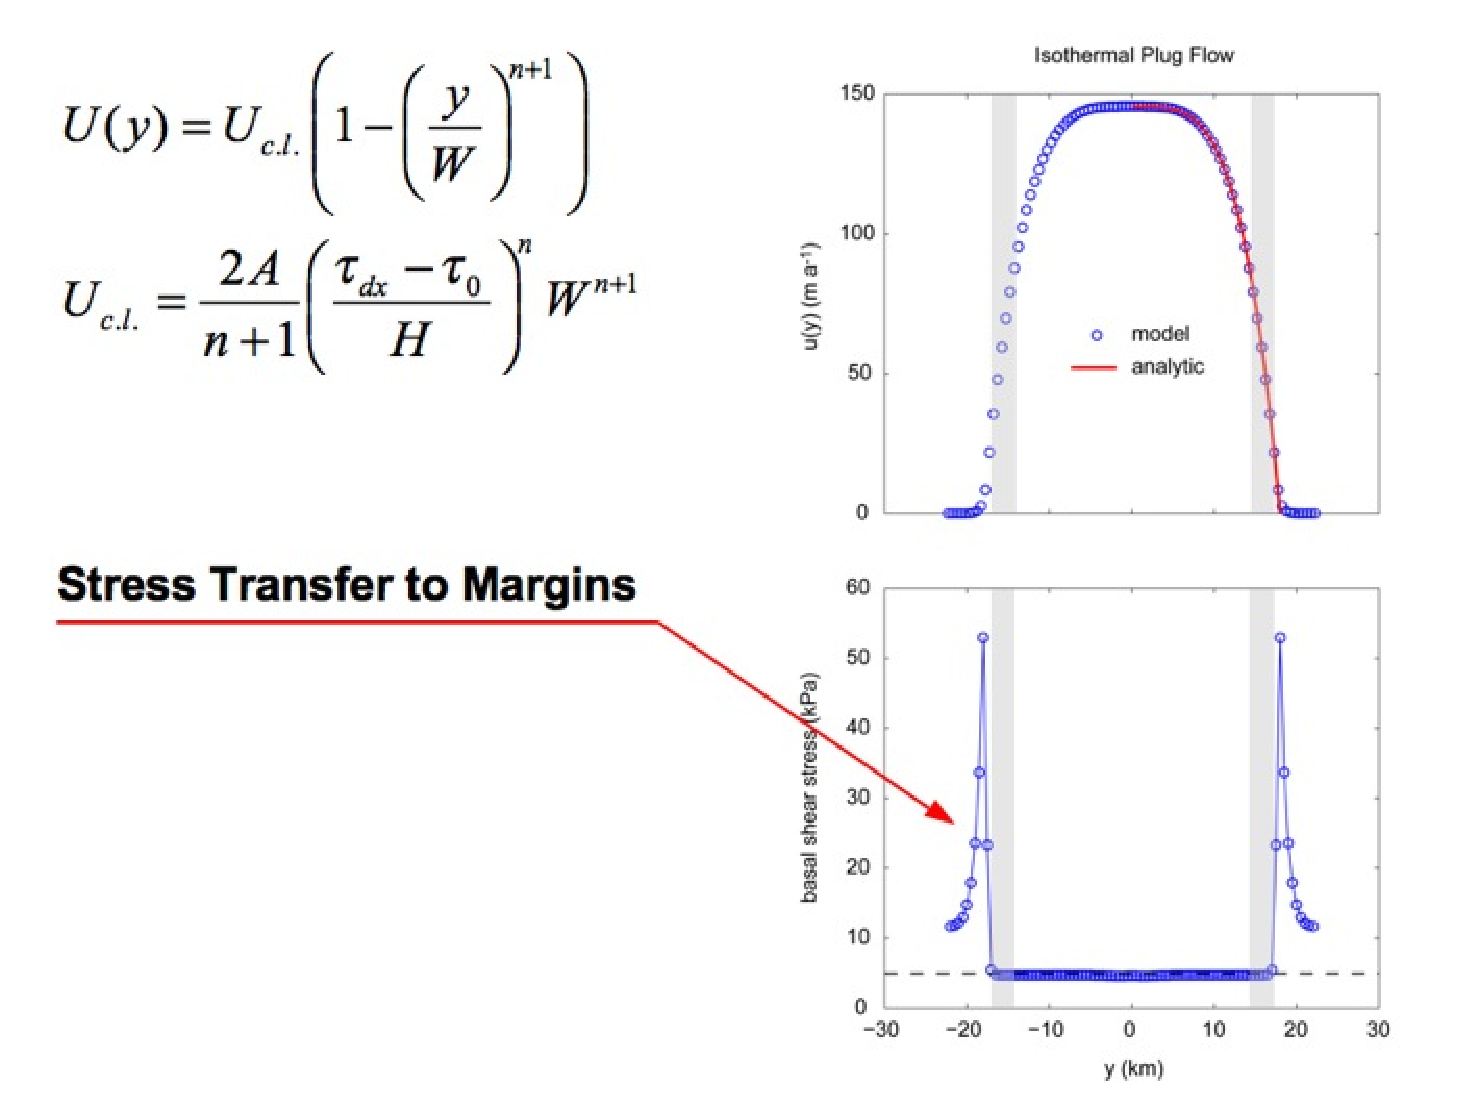
\includegraphics[width=0.65\columnwidth]{\dir/figs/Plastic_bed2.eps}
%  \end{center}
%  \caption{Across-flow profiles of velocity and basal drag from the modeled, idealized ice stream in Figure 1. In the top panel, the analytical solution from \textit{Raymond} (2005) is also shown for comparison. In the bottom panel, stress transfer to the lateral margins is clearly seen.}
%    \label{fig:plasticbed2}
%\end{figure} 

\subsection{Lateral Boundary Conditions}
Currently, the only lateral boundary condition implemented that is of any significance is that for floating ice; the depth-averaged stress resulting from an adjacent column of ocean water is applied at the location of an ice shelf (or ice tongue) front. The derivation follows largely along the lines above for the free surface and specified basal traction boundary conditions, except that the surface normal vectors, $n_{x}$ and $n_{y}$, are taken as lying entirely in the $x$, $y$ plane (that is, they are perpendicular to a vertical shelf front). Thus we have

\begin{equation}
\begin{split}
  & \hat{x}:\quad 4\eta \frac{\partial u}{\partial x}n_{x}+\eta \frac{\partial u}{\partial y}n_{y}+\eta \frac{\partial u}{\partial z}n_{z}=-2\eta \frac{\partial v}{\partial y}n_{x}-\eta \frac{\partial v}{\partial x}n_{y}+\rho g\left( s-z \right)n_{x}-S_{x}, \\ 
 & \hat{y}:\quad 4\eta \frac{\partial v}{\partial y}n_{y}+\eta \frac{\partial v}{\partial x}n_{x}+\eta \frac{\partial v}{\partial z}n_{z}=-2\eta \frac{\partial u}{\partial x}n_{y}-\eta \frac{\partial u}{\partial y}n_{x}+\rho g\left( s-z \right)n_{y}-S_{y} \\ 
\end{split}
\end{equation}

where $S_x$ and $S_y$ are source terms from the pressure due to ocean water (to be defined below) and $\rho g\left( s-z \right)$ comes from including the 1st-order vertical stress balance,

\begin{equation}
\begin{split}
  & \frac{\partial \sigma _{zz}}{\partial z}=\frac{\partial \tau _{zz}}{\partial z}-\frac{\partial P}{\partial z}=\rho g\quad \text{(integrate w}\text{.r}\text{.t}\text{. $z$)}, \\ 
 & P=\rho g\left( s-z \right)+\tau _{zz}, \\ 
 & P=\rho g\left( s-z \right)+2\eta \dot{\varepsilon }_{zz}=\rho g\left( s-z \right)+2\eta \left( -\frac{\partial u}{\partial x}-\frac{\partial v}{\partial y} \right), \\ 
\end{split}
\end{equation}

with \textit{\(\rho{}\)} being the ice density. In the last step above we have used the constitutive relation and incompressibility to expand the vertical, normal-deviatoric stress in terms of the effective viscosity and horizontal-normal strain rates. We calculate the source terms $S_x$ and $S_y$ as the depth-averaged stress at the ice shelf front due to the pressure of ocean water there. This value is given by

\begin{equation}
S_{i}=\left[ \frac{1}{H}\frac{1}{2}\rho _{w}g\left( H-h_f \right)^{2} \right]n_{i}=\left[ \frac{1}{2}\rho _{w}gH\left( \frac{\rho }{\rho _{w}} \right)^{2} \right]n_{i},\quad \quad h_f=H\left( 1-\frac{\rho _{{}}}{\rho _{w}} \right),
\end{equation}

where  \textit{i=x,y}, $n_i$ is the shelf-front normal vector, $H$ is the ice thickness, $h_f$ is the ``freeboard'', or ice thickness above floatation, and $\rho_w$ is the density of ocean water. Because we have taken a depth-average for this source term, we take a depth-average of the term $\rho g\left( s-z \right)$ above, which is $\frac{1}{2}\rho gH$.

Combining these two terms and inserting them in the horizontal boundary condition expressions above gives

\begin{equation}
\begin{split}
& \hat{x}:\quad 4\eta \frac{\partial u}{\partial x}n_{x}+\eta \frac{\partial u}{\partial y}n_{y}+\eta \frac{\partial u}{\partial z}n_{z}= \\
& -2\eta \frac{\partial v}{\partial y}n_{x}-\eta \frac{\partial v}{\partial x}n_{y}+\left[ -\frac{1}{2}H\left( \frac{\rho }{\rho _{w}} \right)^{2}\rho _{w}g+\frac{1}{2}\rho gH \right]n_{x}, \\ 
 & \hat{y}:\quad 4\eta \frac{\partial v}{\partial y}n_{y}+\eta \frac{\partial v}{\partial x}n_{x}+\eta \frac{\partial v}{\partial z}n_{z}= \\
 & -2\eta \frac{\partial u}{\partial x}n_{y}-\eta \frac{\partial u}{\partial y}n_{x}+\left[ -\frac{1}{2}H\left( \frac{\rho }{\rho _{w}} \right)^{2}\rho _{w}g+\frac{1}{2}\rho gH \right]n_{y}, \\ 
\end{split}
\end{equation}

which can be rearranged to

\begin{equation}
\begin{split}
  & \hat{x}:\quad 4\frac{\partial u}{\partial x}n_{x}+\frac{\partial u}{\partial y}n_{y}+\frac{\partial u}{\partial z}n_{z}+2\frac{\partial v}{\partial y}n_{x}+\frac{\partial v}{\partial x}n_{y}=\frac{\rho gH}{2\eta }\left( 1-\frac{\rho }{\rho _{w}} \right)n_{x}, \\ 
 & \hat{y}:\quad 4\frac{\partial v}{\partial y}n_{y}+\frac{\partial v}{\partial x}n_{x}+\frac{\partial v}{\partial z}n_{z}+2\frac{\partial u}{\partial x}n_{y}+\frac{\partial u}{\partial y}n_{x}=\frac{\rho gH}{2\eta }\left( 1-\frac{\rho }{\rho _{w}} \right)n_{y}. \\ 
\end{split}
\end{equation}

For an ice shelf, the surface and basal velocities are equal, in which case the vertical velocity gradient terms are $\sim{0}$, giving the final form of the lateral boundary conditions implemented in the model,

\begin{equation}
\begin{split}
  & \hat{x}:\quad 4\frac{\partial u}{\partial x}n_{x}+\frac{\partial u}{\partial y}n_{y}+2\frac{\partial v}{\partial y}n_{x}+\frac{\partial v}{\partial x}n_{y}=\frac{\rho gH}{2\eta }\left( 1-\frac{\rho }{\rho _{w}} \right)n_{x}, \\ 
 & \hat{y}:\quad 4\frac{\partial v}{\partial y}n_{y}+\frac{\partial v}{\partial x}n_{x}+2\frac{\partial u}{\partial x}n_{y}+\frac{\partial u}{\partial y}n_{x}=\frac{\rho gH}{2\eta }\left( 1-\frac{\rho }{\rho _{w}} \right)n_{y}. \\ 
\end{split}
\end{equation}

\subsection{Summary}
Note that the form for \textit{all} of the boundary conditions above is very similar. In fact, all that differs among the equations for the free surface, the specified basal traction, and the lateral shelf boundary condition is (1) the definition of the normal vectors and (2) the existence and definition of a source term. Here are the \textit{x} direction equations again for the three cases:

\begin{equation}
\begin{split}
  & \hat{x}:\quad 4\frac{\partial u}{\partial x}\frac{\partial s}{\partial x}+ \frac{\partial u}{\partial y}\frac{\partial s}{\partial y}+2 \frac{\partial v}{\partial y}\frac{\partial s}{\partial x}+\frac{\partial v}{\partial x}\frac{\partial s}{\partial y}-\frac{\partial u}{\partial z}=0, \\ 
  & \hat{x}:\quad 4\frac{\partial u}{\partial x}\frac{\partial b}{\partial x}+\frac{\partial u}{\partial y}\frac{\partial b}{\partial y}+2\frac{\partial v}{\partial y}\frac{\partial b}{\partial x}+\frac{\partial v}{\partial x}\frac{\partial b}{\partial y}-\frac{\partial u}{\partial z}=\frac{\tau _{bx}}{\eta }, \\ 
  & \hat{x}:\quad 4\frac{\partial u}{\partial x}n_{x}+\frac{\partial u}{\partial y}n_{y}+2\frac{\partial v}{\partial y}n_{x}+\frac{\partial v}{\partial x}n_{y}=\frac{\rho gH}{2\eta }\left( 1-\frac{\rho }{\rho _{w}} \right)n_{x}. \\
\end{split}
\end{equation}

In the first equation (free surface), the normals are related to the ice sheet surface slope and the source term is zero (which subsequently allows us to divide through by the effective viscosity and remove it from the equations). In the second equation (specified basal traction), the normals are related to the bedrock slopes and the source term is related to the assumed relationship between the basal shear stress and the basal sliding rate. In the last equation, the normals are defined by the shape of the ice-shelf front in map view, the vertical velocity gradient terms are absent, and the source term is related to the pressure from the adjacent column of ocean water.


\section{Numerical Solution of Higher-Order Equations}

\textbf{SP: Note that this will have to be updated by Bill at some point. We might be able to get away with some of what is in here for the short term.}

\subsection{Governing Equations}
The final form of the equations we'd like to solve is:
 
\begin{align*}
 & x: \quad 4\frac{\partial }{\partial x}\left( \eta \frac{\partial u}{\partial x} \right)+\frac{\partial }{\partial y}\left( \eta \frac{\partial u}{\partial y} \right)+\frac{\partial }{\partial z}\left( \eta \frac{\partial u}{\partial z} \right)= \\
 &-2\frac{\partial }{\partial x}\left( \eta \frac{\partial v}{\partial y} \right)-\frac{\partial }{\partial y}\left( \eta \frac{\partial v}{\partial x} \right)+\rho g\frac{\partial s}{\partial x} \\ 
 & y: \quad 4\frac{\partial }{\partial y}\left( \eta \frac{\partial v}{\partial y} \right)+\frac{\partial }{\partial x}\left( \eta \frac{\partial v}{\partial x} \right)+\frac{\partial }{\partial z}\left( \eta \frac{\partial v}{\partial z} \right)= \\
 & -2\frac{\partial }{\partial y}\left( \eta \frac{\partial u}{\partial x} \right)-\frac{\partial }{\partial x}\left( \eta \frac{\partial u}{\partial y} \right)+\rho g\frac{\partial s}{\partial y} \\ 
\end{align*}

\subsection{Coordinate Transform}
For ice sheet modeling, it is convenient to recast the governing equations using a dimensionless, stretched vertical coordinate (often called a sigma coordinates). The stretched vertical coordinate is defined as:

\begin{align*}
\sigma = \frac{(s - z)}{H}.
\end{align*}

This means that at the surface of the ice sheet $\sigma = 0$, and at the base $\sigma = 1$ regardless of the ice thickness.  As a result of this transformation, a coordinate ($x,y,z$) is mapped to ($x',y',\sigma$).  This means that function derivatives must be re-written (using $\frac{\partial f}{\partial x}$ as an example) as:

\begin{align*}
\frac{\partial f}{\partial x} = \frac{\partial f}{\partial x'} \frac{\partial x'}{\partial x} + \frac{\partial f}{\partial y'} \frac{\partial y'}{\partial x} + \frac{\partial f}{\partial \sigma} \frac{\partial \sigma}{\partial x}.
\end{align*}

Similarly for $\frac{\partial f}{\partial y}$ and $\frac{\partial f}{\partial z}$. We can simplify this by assuming that 

\begin{align*}
\frac{\partial x'}{\partial x}, \frac{\partial y'}{\partial y} = 1
\end{align*}

and

\begin{align*}
\frac{\partial x'}{\partial y}, \frac{\partial x'}{\partial z}, \frac{\partial y'}{\partial x}, \frac{\partial y'}{\partial z} = 0,
\end{align*}

which is valid if the bed and surface gradients are not too large. This simplifies the above to:

\begin{align*}
\frac{\partial f}{\partial x} = \frac{\partial f}{\partial x'} + \frac{\partial f}{\partial \sigma}\frac{\partial \sigma}{\partial x},
\end{align*}

\begin{align*}
\frac{\partial f}{\partial y} = \frac{\partial f}{\partial y'} + \frac{\partial f}{\partial \sigma}\frac{\partial \sigma}{\partial y},
\end{align*}

\begin{align*}
\frac{\partial f}{\partial z} = \frac{\partial f}{\partial \sigma}\frac{\partial \sigma}{\partial z}.
\end{align*}

Rescaling parameters $a_{x}$, $a_{y}$, $b_{x}$, $b_{y}$, and $c_{xy}$ are defined. For the $x$ derivative case (the $y$ derivative case is analogous) we have

\begin{align*}
a_{x} = \frac{1}{H}(\frac{\partial s}{\partial x'} - \sigma \frac{\partial H}{\partial x'}),
\end{align*}

\begin{align*}
b_{x} = \frac{\partial a_x}{\partial x'} + a_x \frac{\partial a_x}{\partial \sigma} 
    = \frac{1}{H} (\frac{\partial^2 s}{\partial x'^2} - \sigma \frac{\partial^2 H}{\partial x'^2} - 2a_x \frac{\partial H}{\partial x'}),
\end{align*}

\begin{align*}
c_{xy} = \frac{\partial a_y}{\partial x'} + a_x \frac{\partial a_y}{\partial \sigma} 
       = \frac{\partial a_x}{\partial y'} + a_y \frac{\partial a_x}{\partial \sigma}.
\end{align*}

Using these, expressions for the $x$ derivatives become:

\begin{align*}
\frac{\partial f}{\partial x} = \frac{\partial f}{\partial x'} + a_x \frac{\partial f}{\partial \sigma},
\end{align*}

\begin{align*}
 & \frac{\partial }{\partial x}\left( \eta \frac{\partial u}{\partial x} \right)=\frac{\partial }{\partial \hat{x}}\left( \eta \frac{\partial u}{\partial \hat{x}} \right)+\frac{\partial \sigma }{\partial \hat{x}}\frac{\partial }{\partial \sigma }\left( \eta \frac{\partial u}{\partial \hat{x}} \right)+\frac{\partial \sigma }{\partial \hat{x}}\frac{\partial }{\partial \hat{x}}\left( \eta \frac{\partial u}{\partial \sigma } \right)+ \\
& \left( \frac{\partial \sigma }{\partial \hat{x}} \right)^{2}\frac{\partial }{\partial \sigma }\left( \eta \frac{\partial u}{\partial \sigma } \right)+\left( \frac{\partial _{{}}^{2}\sigma }{\partial \hat{x}_{{}}^{2}} \right)\eta \frac{\partial u}{\partial \sigma }
\end{align*}

where hatted values refer to the coordinate directions in sigma coordinates. Similarly, the first cross-stress term on the RHS is given by

\begin{align*}
&\frac{\partial }{\partial x}\left( \eta \frac{\partial v}{\partial y} \right)=\frac{\partial }{\partial \hat{x}}\left( \eta \frac{\partial v}{\partial \hat{y}} \right)\,+\frac{\partial \sigma }{\partial \hat{x}}\frac{\partial }{\partial \sigma }\left( \eta \frac{\partial v}{\partial \hat{y}} \right)\,+\frac{\partial \sigma }{\partial \hat{y}}\frac{\partial }{\partial \hat{x}}\left( \eta \frac{\partial v}{\partial \sigma } \right)\,+ \\
&\frac{\partial \sigma }{\partial \hat{x}}\frac{\partial \sigma }{\partial \hat{y}}\frac{\partial }{\partial \sigma }\left( \eta \frac{\partial v}{\partial \sigma } \right)\,+\frac{\partial _{{}}^{2}\sigma }{\partial \hat{x}\partial \hat{y}}\eta \frac{\partial v}{\partial \sigma }\,
\end{align*}


One term has become five terms and each one of those is pretty ugly looking on its own. Luckily, there is a lot of symmetry here. Notice that if we wanted to design subroutines to discretize the terms on the RHS, we could re-use a lot of them by either applying them to the correct velocity component (to either the $u$ or the $v$ discretization) or by passing the appropriate arguments (by passing either the grid spacing in the $x$ direction or the $y$ direction, where appropriate).

A similar transform is applied to each of the terms in the governing equations given above. At any point within the grid, the grid spacing, coordinate transform, and viscosity information associated with the unknown velocity components is made discrete using finite differences. This information ultimately equates to coefficients on the unknown velocities, allowing the governing equations over the entire grid (with appropriate discretizations for boundary conditions) to be recast as a system of $n$ equations in $n$ unknowns. In turn, this system is solved using standard linear algebraic methods for large, sparse systems of linear equations.

\subsection{Operating Splitting}
In the governing equations given above, note that for the \textit{x} equation we have moved all terms containing gradients in \textit{v} to the right-hand side (RHS) (and vice-versa for the \textit{y} equation). 

This allows us to solve the equations using an $operator$ $splitting$ approach; for the $x$ equation, we treat $v$ as known (where we take the values of $v$ from the previous iteration, as discussed further below) and solve for $u$, and vice versa when we solve the $y$ equation for $v$. The splitting refers to the fact that we are breaking the multi-dimensional divergence operation into two steps; rather than solving one big matrix equation for $u$ and $v$ simultaneously, we solve two smaller matrix equations in sequence with one of the unknowns treated as a known source term on the RHS of the equation. This procedure was probably more common and important years ago when it was desirable to keep the matrix equations as small as possible for memory management issues. On today's machines, with fewer memory limitations (in particular when dealing with codes designed to run on parallel, distributed memory architectures) this splitting is not necessary and may even lead to some undesirable numerical side effects (i.e. a slow-down in the convergence of iterations used to treat nonlinearity in the governing equations).

A general matrix form of the split equations, where coefficients on the $u$ and $v$ velocity components (i.e. viscosity, grid spacing, scalars) are contained in the block matrices \textbf{A}, is given by 

\begin{align*}
\begin{matrix}
  \left[ \begin{matrix}
   \mathbf{A}_{\mathbf{uu}} & \mathbf{0}  \\
   \mathbf{0} & \mathbf{A}_{\mathbf{vv}}  \\
\end{matrix} \right]\left[ \begin{matrix}
   \mathbf{u}  \\
   \mathbf{v}  \\
\end{matrix} \right]=\left[ \begin{matrix}
   \mathbf{b}_{\mathbf{u}}-\mathbf{A}_{\mathbf{uv}}\mathbf{v}  \\
   \mathbf{b}_{\mathbf{v}}-\mathbf{A}_{\mathbf{vu}}\mathbf{u}  \\
\end{matrix} \right] \\ 
   \\ 
  \mathbf{A}_{\mathbf{uu}}\mathbf{u}=\mathbf{b}_{\mathbf{u}}-\mathbf{A}_{\mathbf{uv}}\mathbf{v},\quad \quad \mathbf{A}_{\mathbf{vv}}\mathbf{v}=\mathbf{b}_{\mathbf{v}}-\mathbf{A}_{\mathbf{vu}}\mathbf{u} \\ 
\end{matrix}
\end{align*}

where the \textbf{uu} subscript denotes block matrices containing coefficients for gradients on \textit{u} in the equation for the \textit{x} component of velocity (i.e. \textit{u}). The subscript \textbf{uv} denotes block matrices containing coefficients for gradients on \textit{v} in the equation for the \textit{x} component of velocity (and similarly for the \textbf{vv} and \textbf{vu} subscripts). On the right-hand side, the single subscripts \textbf{u} and \textbf{v} are attached to the geometric source terms for the \textit{x} and \textit{y} components of velocity, respectively.

\subsection{Solution of the Non-linear System Through a Fixed Point Iteration}
The non-linearity in the equations -- the fact that the coefficients on the velocity components (the viscosity) are dependent on the velocity (or more specifically, the velocity gradients) -- is handled through a fixed-point iteration. A general fixed point iteration for a vector of unknowns \textit{u} can be written as 

\begin{align*}
u^{k}=\mathbf{B}\left( u^{k-1} \right),
\end{align*}

where \textit{k} is the index for the \textit{u} being solved for and \textbf{B} is a matrix operation performed on the components of \textit{u} obtained at the previous iteration, \textit{k-1}. The fixed point occurs when the values of \textit{u} at \textit{k} and \textit{k-1} are equal to within some given tolerance (at which point the iteration process is halted). CISM has options for implementing both Picard and Newton-based fixed-point iterations. For the Picard iteration (standard in CISM), the matrix coefficients with a velocity dependence are simply based on the velocities obtained at the previous iteration. In most cases, this equates to using velocities obtained from the previous iteration to calculate the strain rate components that go into the calculation of the effective viscosity, $\eta$.

\section{Final Matrix Form}
When accounting for both the operator splitting and the Picard iteration on the effective viscosity, the final form of the matrix equations solved in CISM becomes 

\begin{align*}
\begin{matrix}
  \left[ \begin{matrix}
   \mathbf{A}_{\mathbf{uu}}^{k-1} & \mathbf{0}  \\
   \mathbf{0} & \mathbf{A}_{\mathbf{vv}}^{k-1}  \\
\end{matrix} \right]\left[ \begin{matrix}
   \mathbf{u}^{k}  \\
   \mathbf{v}^{k}  \\
\end{matrix} \right]=\left[ \begin{matrix}
   \mathbf{b}_{\mathbf{u}}-\mathbf{A}_{\mathbf{uv}}^{k-1}\mathbf{v}^{k-1}  \\
   \mathbf{b}_{\mathbf{v}}-\mathbf{A}_{\mathbf{vu}}^{k-1}\mathbf{u}^{k-1}  \\
\end{matrix} \right] \\ 
   \\ 
  \mathbf{A}_{\mathbf{uu}}^{k-1}\mathbf{u}=\mathbf{b}_{\mathbf{u}}-\mathbf{A}_{\mathbf{uv}}^{k-1}\mathbf{v}^{k-1},\quad \quad \mathbf{A}_{\mathbf{vv}}^{k-1}\mathbf{v}=\mathbf{b}_{\mathbf{v}}-\mathbf{A}_{\mathbf{vu}}^{k-1}\mathbf{u}^{k-1} \\ 
\end{matrix}
\end{align*}

where the index \textit{k} denotes an unknown value being solved for during the current non-linear iteration and the index \textit{k}-1 denotes a lagged value taken from solution at the end of the previous non-linear iteration (again, here the lagging is primarily with respect to the effective viscosity, the value of which is calculated using velocity gradients obtained at the end of the previous iteration). The final form of the matrix equations given above represents a linear system; for the solution at any particular nonlinear iteration \textit{k}, all of the coefficients on the unknown velocity components \textit{u} and \textit{v} are held frozen during the solution of the linear system. This linear system can be solved using any practical method. For large, sparse systems, some variant on the iterative conjugate gradient method (e.g. BiCG, GMRES) is generally the most efficient. In this case the linear system is not solved exactly but is solved to within some small tolerance of the true solution.

\subsection{Newton-based Methods for Solutions of the Non-linear System}
Without any operator splitting, the generic matrix form of the equations to be solved can be written as

\begin{align*}
\mathbf{A}(\mathbf{u})\mathbf{u}=\mathbf{b}.
\end{align*}

The linearized form of the equations to be solved using the Picard solution can be written as

\begin{align*}
\mathbf{u}^{k}=\mathbf{A}(\mathbf{u}^{k-1})^{-1}\mathbf{b}.
\end{align*}

The full nonlinear system to be solved can be written as

\begin{align*}
\mathbf{F}(\mathbf{u})=\mathbf{A}(\mathbf{u})\mathbf{u}-\mathbf{b}
\end{align*}

with the solution for the uknown vector \textit{u} given by 

\begin{align*}
\mathbf{F}(\mathbf{u})=0.
\end{align*}

A Newton-based solution for this system of equations, based on a first-order Taylor series expansion about the solution for \textit{u} at iteration \textit{k-1}, can be written as

\begin{align*}
\mathbf{F}(\mathbf{u}^{k})=\mathbf{F}(\mathbf{u}^{k-1})+\mathbf{F}(\mathbf{u}^{k-1})\delta \mathbf{u}^{k-1},
\end{align*}

where

\begin{align*}
\mathbf{F}(\mathbf{u}^{k-1})=\mathbf{J}^{k-1}
\end{align*}

is the system Jacobian with individual components give by

\begin{align*}
J_{ij}=\frac{\partial F_{i}(\mathbf{u}^{k-1})}{\partial u_{j}}
\end{align*}

and 

\begin{align*}
\delta \mathbf{u}^{k-1}=\mathbf{u}^{k}-\mathbf{u}^{k-1}
\end{align*}

is the Newton update to be solved for. One method for doing so is by solving 

\begin{align*}
\delta \mathbf{u}^{k-1}=-\left( \mathbf{J}^{k-1} \right)^{-1}\mathbf{F}(\mathbf{u}^{k-1}).
\end{align*}

The advantage of Newton-based methods is that, with a good initial guess for the solution, convergence rates are very often quadratic (e.g. the residual decreases quadratically, so that at iteration \textit{k} one has a residual of 0.1, at iteration \textit{k+1}, a residual of 0.01, and at iteration \textit{k+2} a residual of 0.0001), whereas Picard-based iterations are much slower to converge. A figure comparing rates of convergence for Picard versus Newton on a CISM tests case is shown below (Figure \ref{fig:jfnk}. The Newton method is based on the work of Lemieux et al. ($J.$ $Comput.$ $Phys.$, \textbf{230}, 2011), which is discussed further below.

%\begin{figure}
%  \begin{center}
%    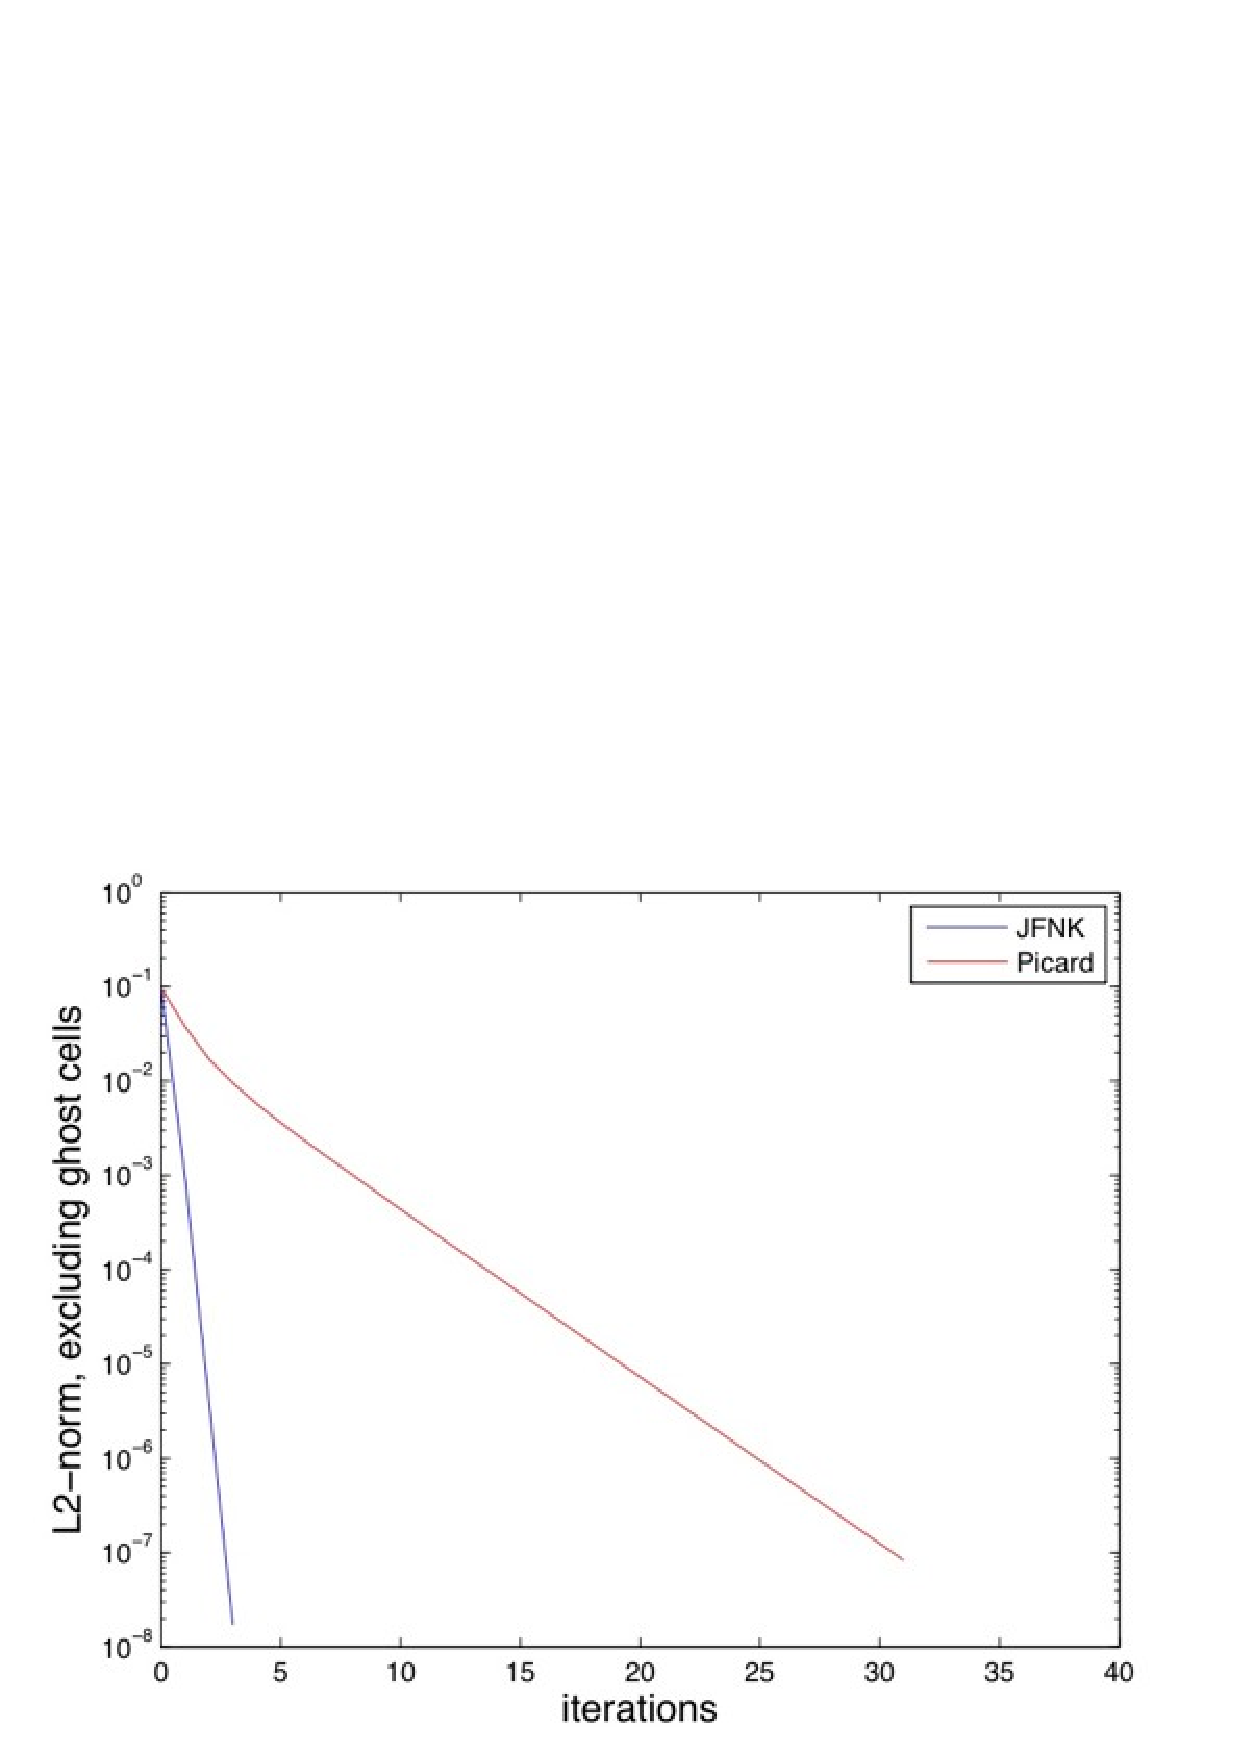
\includegraphics[width=0.9\columnwidth]{\dir/figs/Picard_vs_newton.png}
%  \end{center}
%  \caption{Rates of convergence for the nonlinear iteration in CISM.}
%  \label{fig:jfnk}
%\end{figure} 

\subsection{The Jacobian Free Approach}
In practice, the model Jacobian may either be too difficult or to expensive too form. A Jacobian Free Newton-Krylov (JFNK) approach has recently been implemented in CISM (Leimieux et al., 2011), largely following methods discussed in Knoll and Keyes ($J.$ $Comput.$ $Phys.$, \textbf{193}, 2004).

The crux of the method comes from noting that, when solving the last equation above using a Krylov method (e.g. Conjugate Gradients, GMRES, etc.) the solution for the Newton update is taken from a combination of Krylov vectors that span the subspace


\begin{align*}
span\left\{ \mathbf{r}_{0},\mathbf{Jr}_{0},\mathbf{J}^{2}\mathbf{r}_{0},...,\mathbf{J}^{n-1}\mathbf{r}_{0} \right\}=span\left\{ \mathbf{r}_{0},\mathbf{Jv}_{1},\mathbf{Jv}_{2},...,\mathbf{Jv}_{n-1} \right\}.
\end{align*}

This implies that, when using a Krylov method, one only ever needs to calculate matrix vector products of the form $\mathbf{Jv}$ when building up the subspace that approximates the solution vector $\delta \mathbf{u}$.

Following Knoll and Keyes (2004), note that the necessary matrix vector products can be approximated through nonlinear function evaluations and a perturbation as

\begin{align*}
\mathbf{Jv}\approx \frac{\mathbf{F}\left( \mathbf{u}+\varepsilon \mathbf{v} \right)-\mathbf{F}\left( \mathbf{u} \right)}{\varepsilon }.
\end{align*}

It is not immediately obvious why this approximation is valid. To verify this, take a few steps back and consider a nonlinear system of equations of two variables, $u_{1}$ and $u_{2}$. The right-hand side of the above equation can be expanded as

\begin{align*}
\frac{\mathbf{F}\left( \mathbf{u}+\varepsilon \mathbf{v} \right)-\mathbf{F}\left( \mathbf{u} \right)}{\varepsilon }=\left[ \begin{matrix}
   \frac{F_{1}\left( u_{1}+\varepsilon v_{1},u_{2}+\varepsilon v_{2} \right)-F_{1}(u_{1},u_{2})}{\varepsilon }  \\
   \frac{F_{2}\left( u_{1}+\varepsilon v_{1},u_{2}+\varepsilon v_{2} \right)-F_{2}(u_{1},u_{2})}{\varepsilon }  \\
\end{matrix} \right].
\end{align*}

A first-order Taylor series expansion approximation to this is given by

\begin{align*}
\frac{\mathbf{F}\left( \mathbf{u}+\varepsilon \mathbf{v} \right)-\mathbf{F}\left( \mathbf{u} \right)}{\varepsilon }\approx \left[ \begin{matrix}
   \frac{F_{1}\left( u_{1},u_{2} \right)+\varepsilon v_{1}\frac{\partial F_{1}}{\partial u_{1}}+\varepsilon v_{2}\frac{\partial F_{1}}{\partial u_{2}}-F_{1}(u_{1},u_{2})}{\varepsilon }  \\
   \frac{F_{2}\left( u_{1},u_{2} \right)+\varepsilon v_{1}\frac{\partial F_{2}}{\partial u_{1}}+\varepsilon v_{2}\frac{\partial F_{2}}{\partial u_{2}}-F_{2}(u_{1},u_{2})}{\varepsilon }  \\
\end{matrix} \right],
\end{align*}

which collapses to

\begin{align*}
\frac{\mathbf{F}\left( \mathbf{u}+\varepsilon \mathbf{v} \right)-\mathbf{F}\left( \mathbf{u} \right)}{\varepsilon }\approx\left[ \begin{matrix}
   v_{1}\frac{\partial F_{1}}{\partial u_{1}}+v_{2}\frac{\partial F_{1}}{\partial u_{2}}  \\
   v_{1}\frac{\partial F_{2}}{\partial u_{1}}+v_{2}\frac{\partial F_{2}}{\partial u_{2}}  \\
\end{matrix} \right].
\end{align*}

Finally, note that the right-hand side of the above equation is equal to 

\begin{align*}
\mathbf{Jv}\approx\left[ \begin{matrix}
   v_{1}\frac{\partial F_{1}}{\partial u_{1}}+v_{2}\frac{\partial F_{1}}{\partial u_{2}}  \\
   v_{1}\frac{\partial F_{2}}{\partial u_{1}}+v_{2}\frac{\partial F_{2}}{\partial u_{2}}  \\
\end{matrix} \right],
\end{align*}

with the Jacobian matrix given by

\begin{align*}
\mathbf{J}=\left[ \begin{matrix}
   \frac{\partial F_{1}}{\partial u_{1}} & \frac{\partial F_{1}}{\partial u_{2}}  \\
   \frac{\partial F_{2}}{\partial u_{1}} & \frac{\partial F_{2}}{\partial u_{2}}  \\
\end{matrix} \right].
\end{align*}

The matrix vector product \textbf{Jv} is what needs to be calculated repeatedly while building up the Krylov subspace vectors that combine to approximate the Newton update vector $\delta \mathbf{u}$.

The important point is that at no point in this process does one need to calculate the entire Jacobian matrix. Another important point is that the accuracy of the approximation to the Jacobian is proportional to the small perturbation term, $\varepsilon$.

%\section{References}
%\begin{itemize}
%\item  {Knoll, D.A. and D.E. Keyes. Jacobian-free Newton-Krylov methods: a survey of approaches and applications, \textbf{193}, 357-397, 2004}.
%\end{itemize}
%
%\begin{itemize}
%\item  {Lemieux, J.F., S.F. Price, K.J. Evans, D. Knoll, A.G. Salinger, D. Holland, and A.J. Payne. Implementation of the Jacobian-Free Newton-Krylov method for solving the first-order ice sheet momentum balance, \textit{J. Comput. Phys.}, \textbf{230}, 6531-6545, doi:10.1016/j.jcp.2011.04.037, 2011}.
%\end{itemize}
%
%\end{document}

\section{Thickness Evolution in Higher-Order Models}
\label{sc:ho-thickness-evol}

\subsection{Conservation of mass}
As mentioned previously, conservation of mass for an ice sheet can be expressed by

\begin{align*}
\frac{\partial H}{\partial t}=-\nabla \cdot \left( \vec{U}H \right)+\dot{b},
\end{align*}

where $\vec{U}=(U,V)$ is the 2-dimensional, depth-integrated velocity vector, $H$ is the ice thickness, $\vec{U}H$ is the 2-dimensional ice flux vector, and $\dot{b}$ represents the sum of surface and basal mass balance terms. The change in thickness per unit time is given by the negative of the flux divergence plus a source term. 
%We can expand this a bit as,
%
%\begin{align*}\frac{\partial H}{\partial t}=-\left( \frac{\partial \left( UH \right)}{\partial x}+\frac{\partial \left( VH \right)}{\partial y} \right)+\dot{b}, \\ 
%\end{align*}
%
%where $\vec{U}$ is the depth-averaged velocity vector (in map plane), and \textit{U} and \textit{V} are the depth integrated \textit{x} and \textit{y} velocity fields, \textit{H} is the ice thickness, and $\dot{b}$ is the source term, which is the surface mass balance (>0 for accumulation and <0 for ablation). 
Note that the negative sign in front of the divergence (terms in parentheses on the right-hand side) insures sensible behavior: consider a section of the ice sheet where the thickness is nearly constant and there is no accumulation or ablation. If the velocity gradient along-flow is negative (the ice is slowing down), then we expect local thickening (left-hand side of the equation is $>0$) and vice versa (if the ice is speeding up along flow, we expect local thinning). This is the equation that needs to be solved to calculate the evolution of the ice sheet geometry.

\subsection{A diffusive approach}
For the case of a shallow-ice model, the values of $U$ and $V$ are recast in terms of ice thickness and elevation gradients, in which case the whole problem can be recast as a diffusion equation in ice thickness. In 1-dimension, the equation becomes

\begin{align*}
\frac{\partial H}{\partial t}=\frac{\partial }{\partial x}\left( D\frac{\partial h}{\partial x} \right)+\dot{b},\quad D=\frac{2A}{n+2}\left( \rho g \right)^{n}H^{n+2}\left| \frac{\partial h}{\partial x} \right|^{n-1},
\end{align*}

where $D$ is the non-linear diffusivity (because it depends on the solution to the equation, $H$), $A$ is the rate factor in Glen's flow law, $n$ is the power-law exponent, $h$ is the ice surface elevation, and $\rho$ and $g$ are the ice density and the acceleration due to gravity. Importantly, we need only local information in order to solve the above equation. If our velocity solution can not be solved locally, as in the case of higher-order models, we cannot easily use the above formulation to solve ice sheet evolution. In an attempt to use this form and retain a diffusion-solution approach to the problem (diffusion problems generally have nice numerical properties), we could try the following approach (again, in 1-dimensions only),

\begin{align*}
\frac{\partial H}{\partial t}=\frac{\partial }{\partial x}\left( D\frac{\partial h}{\partial x} \right)+\dot{b},\quad D=UH\left( \frac{\partial h}{\partial x} \right)^{-1},
\end{align*}

where the $U$ in the expression for $D$ is the depth-integrated velocity field from the higher-order model. This is the approach initially taken by \citet{Pattyn:2003tj} in one of the first higher-order modeling studies to deal with this particular problem. Notice that ice sheet surface slope is in the denominator of the diffusivity here and, as slopes get smaller and smaller (as they tend to do in regions of fast flow like ice streams and ice shelves) the diffusivity will get larger and larger (approaching infinity as the slope goes to zero). The faster velocities in these regions appear in the numerator of the diffusivity, also making it larger. This is a severe restriction on this approach because, for explicit schemes, the diffusive CFL condition requires that

\begin{align*}
\Delta t<\frac{\left( \Delta x \right)^{2}}{2D},
\end{align*}

where $\Delta t$ is the time step required for numerical stability and $\Delta x$ is the grid spacing. As the diffusivity goes to infinity (i.e., for faster flows and shallower slopes), the stable time step goes to zero. Thus in practice, this approach has proven very difficult to use for calculating ice sheet evolution in most of the dynamically interesting areas of ice sheets that we are interested in. An alternate approach is needed.

\subsection{Advection schemes}
An alternate approach is to solve the evolution equation using an advection scheme. Numerically, advection schemes can be more problematic than diffusion schemes, but in some cases like this one, they are difficult to avoid. The most general advection scheme is a first-order, upwind-advection scheme (as above, ``first-order" here refers to first-order accurate), and we will outline the implementation of such a scheme below.

Most ice sheet models (and fluid dynamics models in general) perform calculations on a ``staggered" grid of the type shown below in Figure \ref{fig:stag_c_grid}, where velocity components live on one grid and scalar components (e.g. temperatures, pressures, thickness, etc.) live on a grid that is staggered by 1/2 grid space in the horizontal dimensions (this is essential for numerical stability reasons that we won't discuss here).

\begin{figure}
  \begin{center}
    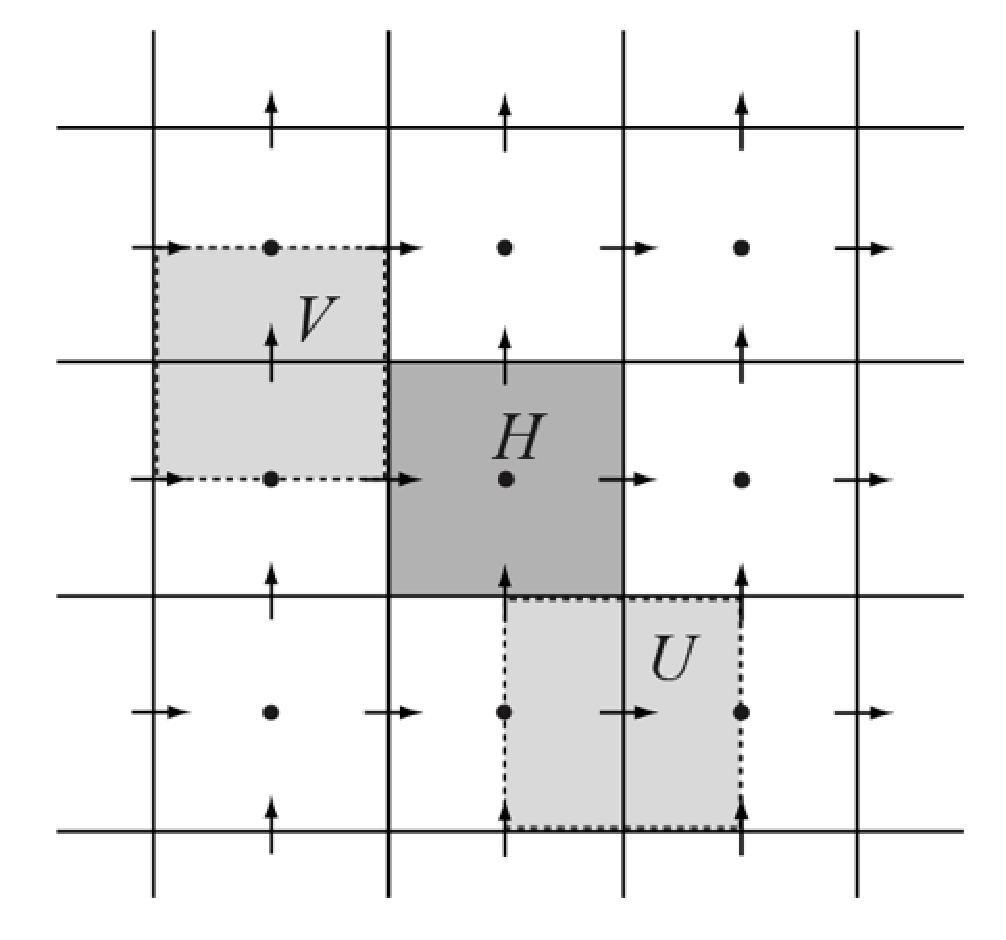
\includegraphics[width=0.4\columnwidth]{\dir/figs/Stag_grid.eps}
  \end{center}
\caption{Staggered grid in two dimensions, showing scalars (like thickness, $H$) at grid cell centers and velocity components, $U$ and $V$, at grid cell faces. This is a ``C" grid. Another staggered-grid possibility is a ``B" grid, for which both velocity components live at the grid cell corners. While CISM uses a B grid, averaging of corner velocities to face centers allows one to express them on a C grid, if necessary.}
  \label{fig:stag_c_grid}
\end{figure} 

A control volume (or finite volume) approach to solving the equation 

\begin{align*}
\frac{\partial H}{\partial t}=-\left( \frac{\partial \left( UH \right)}{\partial x}+\frac{\partial \left( VH \right)}{\partial y} \right)+\dot{b} \\ 
\end{align*}

would be to integrate our equation over a control volume centered on the scalar values (Figures \ref{fig:stag_c_grid} and \ref{fig:stag_c_grid2}). Ignoring source terms for now (assume $\dot{b}=0$), and assuming flow along the \textit{x} direction only (assume $V=0$) we have

\begin{align*}
\frac{\partial H}{\partial t}=-\frac{1}{\Delta y\Delta x}\int_{s}^{n}{\int_{w}^{e}{\frac{\partial \left( UH \right)}{\partial x}}}dxdy=-\frac{1}{\Delta y\Delta x}\left( HU_{e}-HU_{w} \right)\Delta y. \\
\end{align*}

The ``east" and ``west" (subscripts $e$ and $w$) faces of the control volume are shown in Figure \ref{fig:stag_c_grid2}.

\begin{figure}
  \begin{center}
    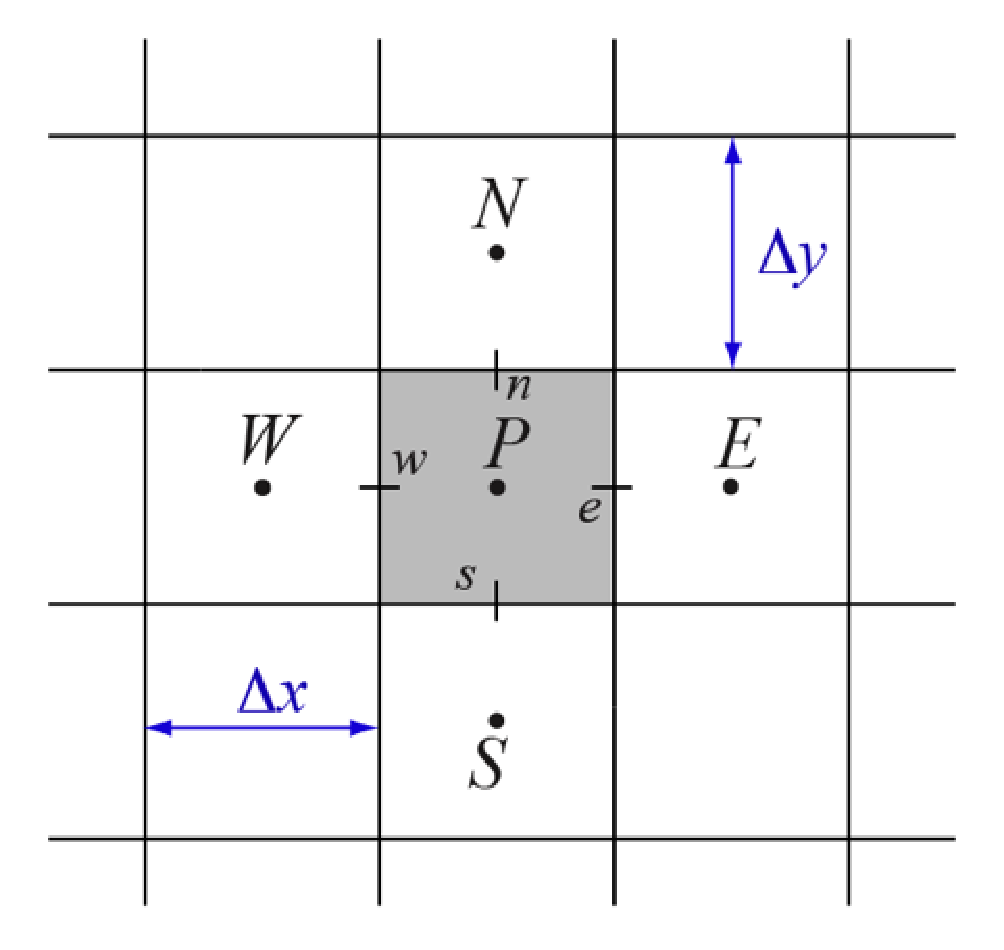
\includegraphics[width=0.4\columnwidth]{\dir/figs/Stag_gridb.eps}
  \end{center}
  \caption{Staggered grid in two dimensions, showing locations of interfaces and control volume dimensions. Interfaces \textit{e}, \textit{w}, \textit{n} and \textit{s} connect the volume centered at \textit{P} with those volumes to the east, west, north, and south (\textit{E}, \textit{W}, \textit{N}, and \textit{S}).}
  \label{fig:stag_c_grid2}
\end{figure} 

In the above equation, we have deliberately left it vague as to which value of $H$ is being advected across the east and west interfaces, into or out of the volume. This is where the term ``upwinding" comes in -- we choose the scalar value to advect across the interface based on an upwinding criterion. If, for example, the flow at interface $e$ is from left to right ($U>0$), we would advect the value of $H$ at $P$ \textit{out} of the volume centered at $P$ and \textit{into} the volume centered at $E$. If, on the other hand, the flow at $e$ was from right to left ($U<0$), we would advect the value of $H$ at $E$ \textit{into} the volume at $P$ and \textit{out} of the volume at $E$. 

The product of velocity, thickness, and the grid spacing at each interface gives a volume flux in units of cubic meters per year. The sum of the volume fluxes over the total number of faces being considered (two in this case, but four for the 2-dimensional case) gives the total volume flux in (total$>$0) or out (total$<$0) of the volume. When this number is divided by the area of the volume, the result is the mean thickness change in that volume, per unit time, that is required to maintain conservation of mass.

\subsection{Explicit vs. Implicit Evolution Schemes}

Is this an explicit or implicit scheme? If we discretize the right-hand side of the primary equation in time we get

\begin{align*}
  & \frac{\partial H}{\partial t}=-\nabla \cdot \left( UH \right)+\dot{b}, \\
 & \frac{H_{t=1}-H_{t=0}}{\Delta t}\approx -\nabla \cdot \left( UH \right)+\dot{b}.\\
\end{align*}

This can be rearranged to,

\begin{align*}
H_{t_{t=1}}\approx H_{t=0}+\left[ -\nabla \cdot \left( UH \right)+\dot{b} \right]_{t=0}\Delta t.
\end{align*}

The thickness at the new time step $t=1$ is a function of \textit{only} variables evaluated at the previous time step $t=0$. Thus, the scheme is \textit{explicit} and, as such, is subject to the advective CFL condition for stability,

\begin{align*}
\Delta t<\frac{\Delta x}{U}.\\
\end{align*}

Essentially, this means that we cannot take such a large time step that we advect mass through more than one volume (past more than one grid space) per time step.

There is not much more to a first-order advection scheme other than extending it to two dimensions for non-zero \textit{V}. The finite volume formulation guarantees that it will be conservative globally (i.e. all mass moved around on the grid is accounted for at each time step). There are many other ``higher-order" advection schemes available (e.g., the incremental remapping scheme used in CISM and described in Chapter \ref{ch:glissade}), but they are mainly based on the principles outlined here and rely on corrections to the simple upwind assumption in order to gain more accuracy.




\chapter{Higher-Order Ice Dynamics: Glissade Dynamical Core}
\renewcommand{\dir}{glissade}

\label{ch:glissade}




\section{Introduction}
\label{sc:glissade-intro}

Some text here

\section{Velocity solver}
\label{sc:glissade-velocity}

Glissade computes the ice velocity by solving an appropriate
approximation of the Stokes equations, given the 2D surface elevation and thickness fields and
the 3D temperature field.
Section (cite section) describes assembly and solution of the matrix problem for the 3D first-order
Blatter-Pattyn approximation.  Section (cite section) then discusses assembly and solution
methods for simpler approximations, including the SIA and SSA.

\subsection{Blatter-Pattyn approximation}

The basic equations of the Blatter-Pattyn approximation in Cartesian coordinates, repeated from Section (cite section), are 

\begin{equation}
  \label{gliss.eq.stress_balance}
  \begin{split}
    x: \quad \frac{\partial }{\partial x}\left( 4 \eta \frac{\partial u}{\partial x} +  2 \eta \frac{\partial v}{\partial y} \right) + \frac{\partial }{\partial y}\left[ \eta \left( \frac{\partial u}{\partial y} + \frac{\partial v}{\partial x} \right) \right]+\frac{\partial }{\partial z}\left( \eta \frac{\partial u}{\partial z} \right) = \rho g\frac{\partial s}{\partial x}, \\
    y: \quad \frac{\partial }{\partial y}\left( 4 \eta \frac{\partial v}{\partial y} +  2 \eta \frac{\partial u}{\partial x} \right) + \frac{\partial }{\partial x}\left[ \eta \left( \frac{\partial u}{\partial y} + \frac{\partial v}{\partial x} \right) \right]+\frac{\partial }{\partial z}\left( \eta \frac{\partial v}{\partial z} \right) = \rho g\frac{\partial s}{\partial y},  \\
  \end{split}
\end{equation}

\noindent
where $u$ and $v$ are the components of horizontal velocity, $\eta$ is the effective viscosity, $s$ is the ice surface elevation,
$\rho$ is the density of ice (assumed constant), and $g$ is gravitational acceleration.  

As in Glide, the equations are discretized on two structured, rectangular horizontal meshes: an unstaggered mesh
of dimension $(nx,ny)$ and a staggered mesh of dimension $(nx-1,ny-1)$.  The rectangles
are called \textit{cells}, and the corners of each cell (where four rectangles meet) are called \textit{vertices}.
The vertical levels of the mesh are based on a terrain-following sigma coordinate system (insert sigma equation).
There are $nz$ \textit{levels} in the vertical direction, with $nz-1$ \textit{layers} between these levels.
An \textit{element} is the region associated with a particular cell and layer; there are
$(nx)(ny)(nz-1)$ elements on the mesh.  A \textit{node} is a point where eight elements intersect (or where four elements
intersect at the upper or lower surface). There are $(nx-1)(ny-1)(nz)$ nodes on the mesh.

Scalar 2D fields such as ice thickness $H$ and surface elevation $s$ are defined for each cell.
Scalar 3D fields such as ice temperature $T$ lie at the center of each element (i.e., in each layer
associated with each cell). Gradients of 2D scalar fields (e.g., the surface slope $\nabla s$) are defined at vertices.
The velocity components $u$ and $v$ live at nodes.

An \textit{active cell} is a cell whose ice thickness exceeds a minimum threshold.  Each active cell is associated with
a column of $nz-1$ active elements.  An \textit{active vertex} is any vertex of an active cell.  Each active vertex is
associated with $nz$ active nodes, including nodes at the surface and bed.

The effective viscosity is defined in each active element by

\begin{equation}
  \label{gliss.eq.effective_viscosity}
  \eta \equiv \frac{1}{2} A^{\frac{-1}{n}} \dot{\varepsilon }_{e}^{\frac{1-n}{n}},
\end{equation}

\noindent
where $A$ is the temperature-dependent rate factor in Glen's flow law, and $\dot{\varepsilon }_{e}$ is the effective strain rate,
given in the Blatter-Pattyn approximation by 

\begin{equation}
  \label{gliss.eq.effective_strain_rate}
        {{\dot{\varepsilon }}^{2}}_{e}={{\dot{\varepsilon }}^{2}}_{xx}+{{\dot{\varepsilon }}^{2}}_{yy}+{{\dot{\varepsilon }}_{xx}}{{\dot{\varepsilon }}_{yy}}+{{\dot{\varepsilon }}^{2}}_{xy}+{{\dot{\varepsilon }}^{2}}_{xz}+{{\dot{\varepsilon }}^{2}}_{yz},
\end{equation}

\noindent
where

\begin{equation}
  \dot{\varepsilon }_{ij} = \frac{1}{2}\left( \frac{\partial u_{i}}{\partial x_{j}} + \frac{\partial u_{j}}{\partial x_{i}} \right).
\end{equation}

\noindent

Given $T$, $s$, $H$, and an initial guess for $u$ and $v$, the problem is to solve Eq. \eqref{gliss.eq.stress_balance}
for $u$ and $v$ at each active node.  (At inactive nodes we assume $u=v=0$.)  This problem can be written in the form

\begin{equation}
  \mathbf{A} \mathbf{x} = \mathbf{b},
\end{equation}

\noindent
or more fully,

\begin{equation}
  \label{gliss.eq.matrix}
  \begin{matrix}
    \left[ \begin{matrix}
        \mathbf{A}_{\mathbf{uu}} & \mathbf{A}_{\mathbf{uv}}  \\
        \mathbf{A}_{\mathbf{vu}} & \mathbf{A}_{\mathbf{vv}}  \\
      \end{matrix} \right]\left[ \begin{matrix}
        \mathbf{u}  \\
        \mathbf{v}  \\
      \end{matrix} \right]=\left[ \begin{matrix}
        \mathbf{b}_{\mathbf{u}}  \\
        \mathbf{b}_{\mathbf{v}}  \\
      \end{matrix} \right], \\ 
    \\ 
    \mathbf{A}_{\mathbf{uu}}\mathbf{u} + \mathbf{A}_{\mathbf{uv}}\mathbf{v} =\mathbf{b}_{\mathbf{u}},
    \quad \quad \mathbf{A}_{\mathbf{vu}}\mathbf{u} + \mathbf{A}_{\mathbf{vv}}\mathbf{v} =\mathbf{b}_{\mathbf{v}}. \\ 
  \end{matrix}
\end{equation}

\noindent
Eq. \eqref{gliss.eq.matrix} explicitly shows the four parts of the total matrix $\mathbf{A}$,
with the solution and right-hand-side vectors separated into $u$ and $v$ components.
In Glissade, $\mathbf{A}$ is always symmetric and positive-definite.

Since $\mathbf{A}$ depends (through $\eta$) on $u$ and $v$, the problem is nonlinear and must be solved iteratively
as described in Section (insert section ref).  For a given nonlinear iteration, we compute $\eta$ based on the
current guess for the velocity field and solve a linear problem of the form \eqref{gliss.eq.matrix}.
Then we update $\eta$ and repeat until the solution converges to within a given tolerance.  This procedure
is known as Picard iteration.

The following sections describe how the matrix equations are assembled and solved. 

\subsubsection{Assembly}

The coupled PDEs \eqref{gliss.eq.stress_balance} are discretized using the finite-element method.
Here we give a detailed but non-rigorous description of the method as applied to the Blatter-Pattyn
approximation on the CISM mesh.
We refer the reader to standard texts (one or two references here) for a full discussion of finite elements.

The PDEs, with appropriate boundary conditions, are solved by dividing the full domain into 
subdomains, or elements, and representing the solution on each element.
On the CISM mesh, the elements are hexahedra (rectangles
in map view), each of which has eight nodes that are shared with its neighbors.
The solution is approximated as a sum over basis functions $\varphi$. One basis function
is associated with each active node.  Its value is $\varphi = 1$ at that node,
with $\varphi = 0$ at all other nodes. The solution at a given point
within an element can be represented as a sum of basis functions multiplied by nodal values:

\begin{equation}
\label{gliss.eq.velo_expansion}  
   u=\sum\limits_{n}{{{\varphi }_{n}}{{u}_{n}}}, \quad v=\sum\limits_{n}{{{\varphi }_{n}}{{v}_{n}}},  \\
\end{equation}

\noindent
where the sum is over the nodes of the element, $u_n$ and $v_n$ are nodal
values of the solution, and $\varphi_n$ varies smoothly between 0 and 1 within the element.
The fact that $\varphi = 0$ except in a small region ensures that the sum includes only
as many terms as there are nodes per element.

Glissade uses standard finite-element techniques to represent the PDE on each element and assemble
the element equations into a global set of algebraic equations of the form \eqref{gliss.eq.matrix}.
The scheme is formally equivalent to that described by \citet{Perego2012} (henceforth PGB).
Note that \eqref{gliss.eq.stress_balance} can be written as

\begin{equation}
  \label{gliss.eq.Perego12}
  \begin{split}
    -\nabla \cdot (2\eta {{{\dot{\varepsilon }}}_{1}}) = -\rho g\frac{\partial s}{\partial x}, \\
    -\nabla \cdot (2\eta {{{\dot{\varepsilon }}}_{2}}) = -\rho g\frac{\partial s}{\partial y}, \\
  \end{split}
\end{equation}

\noindent
where

\begin{equation}
  \label{gliss.eq.Perego13}
  {{{\dot{\varepsilon }}}_{1}}=\left[ \begin{matrix}
      2{{{\dot{\varepsilon }}}_{xx}}+{{{\dot{\varepsilon }}}_{yy}} \\ 
      {{{\dot{\varepsilon }}}_{xy}} \\ 
      {{{\dot{\varepsilon }}}_{xz}} \\ 
    \end{matrix} \right], \quad
  {{{\dot{\varepsilon }}}_{2}}=\left[ \begin{matrix}
      {{{\dot{\varepsilon }}}_{xy}} \\ 
      {{{\dot{\varepsilon }}}_{xx}}+2{{{\dot{\varepsilon }}}_{yy}} \\ 
      {{{\dot{\varepsilon }}}_{yz}} \\ 
    \end{matrix} \right].  \\
\end{equation}

\noindent
(These are Eqs. 12 and 13 in PGB.)  We rewrite the equations in \textit{weak form} (see PGB Eq. 15), which
is obtained by multiplying \eqref{gliss.eq.Perego12} by the basis functions and integrating over the domain, using 
integration by parts to eliminate the second derivative:

\begin{equation}
  \label{gliss.eq.weak_form}
  \begin{split}
    x: \quad \int\limits_{\Omega }{2\eta {{{\dot{\varepsilon }}}_{1}}(u,v)\cdot \nabla {{\varphi }_{1}}\text{ }d\Omega }+\int\limits_{{{\Gamma }_{\beta }}}{\beta u{{\varphi }_{1}}d\Gamma +\int\limits_{\Omega }{\rho g\frac{\partial s}{\partial x}}}{{\varphi }_{1}}\text{ d}\Omega =\text{0},  \\
    y: \quad \int\limits_{\Omega }{2\eta {{{\dot{\varepsilon }}}_{2}}(u,v)\cdot \nabla {{\varphi }_{2}}\text{ }d\Omega }+\int\limits_{{{\Gamma }_{\beta }}}{\beta v{{\varphi }_{2}}d\Gamma +\int\limits_{\Omega }{\rho g\frac{\partial s}{\partial y}}}{{\varphi }_{2}}\text{ d}\Omega =\text{0},  \\
  \end{split}
\end{equation}

\noindent
where $\Omega$ represents the domain volume, $\Gamma$ denotes the lower boundary, and $\beta$ is a basal traction parameter
that can vary spatially.  These equations can also be obtained from a variational principle as described by \citet{DUKOWICZ:2010wb}.

Next we rewrite \eqref{gliss.eq.weak_form} in terms of velocity components.
The first terms on the left-hand-side for the $x$ and $y$ components, respectively, are

\begin{equation}
  \label{gliss.eq.weak_form_velo}
  \begin{aligned}
    & x: \int\limits_{\Omega }{2\eta \left[ \begin{matrix}
          2\frac{\partial u}{\partial x}+\frac{\partial v}{\partial y} & \frac{1}{2}\left( \frac{\partial u}{\partial y}+\frac{\partial v}{\partial x} \right) & \frac{1}{2}\frac{\partial u}{\partial z}  \\
\end{matrix} \right]}\left\{ \begin{matrix}
      \frac{\partial \varphi }{\partial x}  \\[6pt]
      \frac{\partial \varphi }{\partial y}  \\[6pt]
      \frac{\partial \varphi }{\partial z}  \\
    \end{matrix} \right\},  \\
    & y: \int\limits_{\Omega }{2\eta \left[ \begin{matrix}
          \frac{1}{2}\left( \frac{\partial u}{\partial y}+\frac{\partial v}{\partial x} \right) & 2\frac{\partial v}{\partial y}+\frac{\partial u}{\partial x} & \frac{1}{2}\frac{\partial v}{\partial z}  \\
        \end{matrix} \right]}\left\{ \begin{matrix}
      \frac{\partial \varphi }{\partial x}  \\[6pt]
      \frac{\partial \varphi }{\partial y}  \\[6pt]
      \frac{\partial \varphi }{\partial z}  \\
    \end{matrix} \right\},  \\
  \end{aligned}
\end{equation}

\noindent
where brackets denote row vectors and braces denote column vectors.
We will evaluate \eqref{gliss.eq.weak_form_velo} for each active element.  Recall that hexahedral elements have eight nodes,
with $u$ and $v$ to be determined at each active node.
Inserting the velocity expressions \eqref{gliss.eq.velo_expansion} in \eqref{gliss.eq.weak_form_velo}, we obtain

\begin{equation}
  \label{gliss.eq.element_matrix}
  \begin{split}
    x: \int\limits_{\Omega }{2\eta \left( \frac{\partial {{\varphi }_{i}}}{\partial x}\left( 2\left[ \frac{\partial {{\varphi }_{j}}}{\partial x} \right]\left\{ {{u}_{j}} \right\}+\left[ \frac{\partial {{\varphi }_{j}}}{\partial y} \right]\left\{ {{v}_{j}} \right\} \right)+\frac{\partial {{\varphi }_{i}}}{\partial y}\left( \frac{1}{2}\left[ \frac{\partial {{\varphi }_{j}}}{\partial y} \right]\left\{ {{u}_{j}} \right\}+\frac{1}{2}\left[ \frac{\partial {{\varphi }_{j}}}{\partial x} \right]\left\{ {{v}_{j}} \right\} \right)+\frac{\partial {{\varphi }_{i}}}{\partial z}\left( \frac{1}{2}\left[ \frac{\partial {{\varphi }_{j}}}{\partial z} \right]\left\{ {{u}_{j}} \right\} \right) \right)},  \\
    y: \int\limits_{\Omega }{2\eta \left( \frac{\partial {{\varphi }_{i}}}{\partial y}\left( 2\left[ \frac{\partial {{\varphi }_{j}}}{\partial y} \right]\left\{ {{v}_{j}} \right\}+\left[ \frac{\partial {{\varphi }_{j}}}{\partial x} \right]\left\{ {{u}_{j}} \right\} \right)+\frac{\partial {{\varphi }_{i}}}{\partial x}\left( \frac{1}{2}\left[ \frac{\partial {{\varphi }_{j}}}{\partial x} \right]\left\{ {{v}_{j}} \right\}+\frac{1}{2}\left[ \frac{\partial {{\varphi }_{j}}}{\partial y} \right]\left\{ {{u}_{j}} \right\} \right)+\frac{\partial {{\varphi }_{i}}}{\partial z}\left( \frac{1}{2}\left[ \frac{\partial {{\varphi }_{j}}}{\partial z} \right]\left\{ {{v}_{j}} \right\} \right) \right)}.  \\
  \end{split}
\end{equation}

\noindent
Each row or column vector has eight terms, one for each node of the element.

The terms in \eqref{gliss.eq.element_matrix} can be computed to give the terms of a set of four $8\text{x}8$ element matrices.
Each row of an element matrix is associated with $u$ or $v$ at a given node.  The columns in that row contain terms
linking that node to $u$ or $v$ at the other nodes of the element (with the diagonal term linking the node to itself).  

In the $x$ component of \eqref{gliss.eq.element_matrix}, 
the terms in row $i$ that multiply $u_j$ are given by
 
\begin{equation}
  \label{gliss.eq.matrix_Kuu}
  \int\limits_{\Omega }{\eta \left( 4\frac{\partial {{\varphi }_{i}}}{\partial x}\frac{\partial {{\varphi }_{j}}}{\partial x}+\frac{\partial {{\varphi }_{i}}}{\partial y}\frac{\partial {{\varphi}_{j}}}{\partial y}+\frac{\partial {{\varphi }_{i}}}{\partial z}\frac{\partial {{\varphi }_{j}}}{\partial z} \right)}d\Omega
\end{equation}

\noindent
Letting $i$ and $j$ range from 1 to 8, \eqref{gliss.eq.matrix_Kuu} gives the 64 terms of the $8\text{x}8$ element matrix $K_{uu}$,
which links the $u$ value at each node to the $u$ values at all eight nodes.
Similarly, the 64 terms of element matrix $K_{uv}$, which links $u$ at a given node to $v$ at all eight nodes,
are given by

\begin{equation}
  \label{gliss.eq.matrix_Kuv}
  \int\limits_{\Omega }{\eta \left( 2\frac{\partial {{\varphi }_{i}}}{\partial x}\frac{\partial {{\varphi }_{j}}}{\partial y}+\frac{\partial {{\varphi }_{i}}}{\partial y}\frac{\partial {{\varphi }_{j}}}{\partial x} \right)}d\Omega
\end{equation}

Likewise, two $8\text{x}8$ matrices are associated with the $y$ equation in \eqref{gliss.eq.element_matrix}.  
The terms of $K_{vu}$, which connects $v$ at a given node to $u$ at all eight nodes, are given by

\begin{equation}
  \label{gliss.eq.matrix_Kvu}
  \int\limits_{\Omega }{\eta \left( 2\frac{\partial {{\varphi }_{i}}}{\partial y}\frac{\partial {{\varphi }_{j}}}{\partial x}+\frac{\partial {{\varphi }_{i}}}{\partial x}\frac{\partial {{\varphi }_{j}}}{\partial y} \right)}d\Omega
\end{equation}

\noindent
Finally, the terms of $K_{vv}$, which links $v$ at a given node to $v$ at all eight nodes, are given by

\begin{equation}
  \label{gliss.eq.matrix_Kvv}
  \int\limits_{\Omega }{\eta \left( 4\frac{\partial {{\varphi }_{i}}}{\partial y}\frac{\partial {{\varphi }_{j}}}{\partial y}+\frac{\partial {{\varphi }_{i}}}{\partial x}\frac{\partial {{\varphi}_{j}}}{\partial x}+\frac{\partial {{\varphi }_{i}}}{\partial z}\frac{\partial {{\varphi }_{j}}}{\partial z} \right)}d\Omega
\end{equation}

Because of the symmetry of the underlying PDEs, $K_{uu}$ and $K_{vv}$ are symmetric,
and $K_{uv} = K_{vu}^{T}$.  Note that $K_{vv}$ can be obtained from $K_{uu}$, and
$K_{vu}$ from $K_{uv}$, simply by exchanging $x$ and $y$.  The terms
containing $z$ (i.e., the vertical shear stresses associated with the shallow-ice approximation)
appear only in $K_{uu}$ and $K_{vv}$.  The terms containing $x$ and $y$ (i.e.,
the membrane stresses) appear in all four element matrices.

Eqs. \eqref{gliss.eq.matrix_Kuu}--\eqref{gliss.eq.matrix_Kvv} lie at the heart of the code 
(in subroutine \textit{compute\_element\_matrix} of module \textit{glissade\_velo\_higher.F90}).
Together with the expressions for the effective viscosity $\eta$ (discussed below),
these expressions contain the physical contents specific to the Blatter-Pattyn approximation. 

Given the weak form \eqref{gliss.eq.weak_form} of the equations, each of the 64 coefficients in each
element matrix must be integrated over the element.  (Since $\varphi$ varies over the element,
the integrands in \eqref{gliss.eq.matrix_Kuu}--\eqref{gliss.eq.matrix_Kvv} 
have a different value at each point.)  
This is done for a given element by evaluating the integrand at each of 
eight \textit{quadrature points} and taking a weighted sum over quadrature points.
We have to specify the form of the basis functions, then transform the basis functions to
the geometry of the element (which is irregular in the vertical because of the sigma
coordinate) and evaluate the basis function derivatives at the quadrature points.

Glissade uses trilinear basis functions defined on a reference hexahedron.  
This hexahedron is centered at the origin $(0,0,0)$ in local reference coordinates 
$(\hat{x}, \hat{y}, \hat{z}$). 
The eight nodes are located at $(\hat{x}, \hat{y}, \hat{z}) = (\pm 1, \pm 1, \pm 1)$.
By convention, nodes 1--4 are the nodes of the lower face, proceeding counterclockwise
from the southwest corner $(\hat{x}, \hat{y}) = (±1, ±1)$, and nodes 5--8 are the nodes
of the upper face, also moving counterclockwise from the southwest corner.
Thus we have

\begin{equation}
  \label{gliss.eq.basis_functions}
  \begin{matrix}
    {{\varphi }_{1}}=(1-\hat{x})(1-\hat{y})(1-\hat{z})/8,  \\[3pt]
    {{\varphi }_{2}}=(1+\hat{x})(1-\hat{y})(1-\hat{z})/8,  \\[3pt]
    {{\varphi }_{3}}=(1+\hat{x})(1+\hat{y})(1-\hat{z})/8,  \\[3pt]
    {{\varphi }_{4}}=(1-\hat{x})(1+\hat{y})(1-\hat{z})/8,  \\[3pt]
    {{\varphi }_{5}}=(1-\hat{x})(1-\hat{y})(1+\hat{z})/8,  \\[3pt]
    {{\varphi }_{6}}=(1+\hat{x})(1-\hat{y})(1+\hat{z})/8,  \\[3pt]
    {{\varphi }_{7}}=(1+\hat{x})(1+\hat{y})(1+\hat{z})/8,  \\[3pt]
    {{\varphi }_{8}}=(1-\hat{x})(1+\hat{y})(1+\hat{z})/8.  \\
  \end{matrix}
\end{equation} 

\noindent
It is easy to see that for each $n$ we have $\varphi_n = 1$ at a single node, with $\varphi_n = 0$ at the other nodes.

The integrands in \eqref{gliss.eq.matrix_Kuu}--\eqref{gliss.eq.matrix_Kvv} 
are written in terms of real Cartesian coordinates $(x,y,z)$ rather than reference coordinates. 
Spatial derivatives in real coordinates are related to spatial derivatives in reference coordinates by

\begin{equation}
  \label{gliss.eq.real_to_reference}
  \scalebox{1.2}{
    $
  \left\{ \begin{matrix}
    \frac{\partial {{\varphi }_{n}}}{\partial \hat{x}}  \\[6pt]
    \frac{\partial {{\varphi }_{n}}}{\partial \hat{y}}  \\[6pt]
    \frac{\partial {{\varphi }_{n}}}{\partial \hat{z}}  \\
  \end{matrix} \right\} = 
  \left[ \begin{matrix}
      \frac{\partial x}{\partial \hat{x}} & \frac{\partial y}{\partial \hat{x}} & \frac{\partial z}{\partial \hat{x}}  \\[6pt]
      \frac{\partial x}{\partial \hat{y}} & \frac{\partial y}{\partial \hat{y}} & \frac{\partial z}{\partial \hat{y}}  \\[6pt]
      \frac{\partial x}{\partial \hat{z}} & \frac{\partial y}{\partial \hat{z}} & \frac{\partial z}{\partial \hat{z}}  \\
    \end{matrix} \right]
  \left\{ \begin{matrix}
    \frac{\partial {{\varphi }_{n}}}{\partial x}  \\[6pt]
    \frac{\partial {{\varphi }_{n}}}{\partial y}  \\[6pt]
    \frac{\partial {{\varphi }_{n}}}{\partial z}  \\
  \end{matrix} \right\} =
   [J]\left\{ \begin{matrix}
     \frac{\partial {{\varphi }_{n}}}{\partial x}  \\[6pt]
     \frac{\partial {{\varphi }_{n}}}{\partial y}  \\[6pt]
     \frac{\partial {{\varphi }_{n}}}{\partial z}  \\
   \end{matrix} \right\},
   $
  }
\end{equation}

\noindent
where $[J]$ is the Jacobian of the transformation between coordinate systems.  
Given the finite-element expansion

\begin{equation}
   x = \sum\limits_{n}{{{\varphi }_{n}}{{x}_{n}}},
\end{equation}

\noindent
we can evaluate $[J]$ at point $(\hat{x},\hat{y},\hat{z})$ as

\begin{equation}
  \scalebox{1.2}{
  $
  \label{gliss.eq.Jacobian_eval}
        [J(\hat{x},\hat{y},\hat{z})]=\left[ \begin{matrix}
            \sum\limits_{n=1}^{8}{\frac{\partial {{\varphi }_{n}}}{\partial \hat{x}}{{x}_{n}}} & \sum\limits_{n=1}^{8}{\frac{\partial {{\varphi }_{n}}}{\partial \hat{x}}{{y}_{n}}} & \sum\limits_{n=1}^{8}{\frac{\partial {{\varphi }_{n}}}{\partial \hat{x}}{{z}_{n}}}  \\[6pt]
            \sum\limits_{n=1}^{8}{\frac{\partial {{\varphi }_{n}}}{\partial \hat{y}}{{x}_{n}}} & \sum\limits_{n=1}^{8}{\frac{\partial {{\varphi }_{n}}}{\partial \hat{y}}{{y}_{n}}} & \sum\limits_{n=1}^{8}{\frac{\partial {{\varphi }_{n}}}{\partial \hat{y}}{{z}_{n}}}  \\[6pt]
            \sum\limits_{n=1}^{8}{\frac{\partial {{\varphi }_{n}}}{\partial \hat{z}}{{x}_{n}}} & \sum\limits_{n=1}^{8}{\frac{\partial {{\varphi }_{n}}}{\partial \hat{z}}{{y}_{n}}} & \sum\limits_{n=1}^{8}{\frac{\partial {{\varphi }_{n}}}{\partial \hat{z}}{{z}_{n}}}  \\
          \end{matrix} \right].
        $
        }
\end{equation}

Given the derivatives of $\varphi$ at $(\hat{x},\hat{y},\hat{z})$, we can compute the sums
in \eqref{gliss.eq.Jacobian_eval} and invert \eqref{gliss.eq.real_to_reference} to obtain the 
basis function derivatives in terms of $(x,y,z)$:

\begin{equation}
  \label{gliss.eq.reference_to_real}
  \scalebox{1.2}{
    $
  \left\{ \begin{matrix}
     \frac{\partial {{\varphi }_{n}}}{\partial x}  \\[6pt]
     \frac{\partial {{\varphi }_{n}}}{\partial y}  \\[6pt]
     \frac{\partial {{\varphi }_{n}}}{\partial z}  \\
  \end{matrix} \right\} =
          [J^{-1}]  \left\{ \begin{matrix}
    \frac{\partial {{\varphi }_{n}}}{\partial \hat{x}}  \\[6pt]
    \frac{\partial {{\varphi }_{n}}}{\partial \hat{y}}  \\[6pt]
    \frac{\partial {{\varphi }_{n}}}{\partial \hat{z}}  \\
  \end{matrix} \right\}. 
          $
          }
\end{equation}

\noindent
The left-hand side of \eqref{gliss.eq.reference_to_real} contains the terms needed to evaluate
element matrix coefficients in \eqref{gliss.eq.matrix_Kuu}--\eqref{gliss.eq.matrix_Kvv}.

Eqs. \eqref{gliss.eq.matrix_Kuu}--\eqref{gliss.eq.matrix_Kvv} also contain the viscosity $\eta$,
which must be evaluated at each quadrature point.
In the Blatter-Pattyn approximation $\eta$ is given by \eqref{gliss.eq.effective_viscosity};
it is a function of the flow factor $A$ and the effective strain rate defined by \eqref{gliss.eq.effective_strain_rate}.
We approximate $A$ by its value at the element center, where $T$ is defined.
The (squared) effective strain rate, ${{\dot{\varepsilon }}^{2}}_{e}$, is found at each quadrature point
by summing over strain-rate components.  We have

\begin{equation}
  \label{gliss.eq.strain_rates}
  \frac{\partial u}{\partial x}=\sum\limits_{n=1}^{8}{\frac{\partial {{\varphi }_{n}}}{\partial x}}{{u}_{n}}, \quad
  \frac{\partial v}{\partial x}=\sum\limits_{n=1}^{8}{\frac{\partial {{\varphi }_{n}}}{\partial x}}{{v}_{n}},
\end{equation}

\noindent
and similarly for the $y$ and $z$ derivatives.

We now have the tools needed to evaluated the integrands \eqref{gliss.eq.matrix_Kuu}--\eqref{gliss.eq.matrix_Kvv}
at quadrature points. For integrating over a hexahedron, there are eight quadrature points are located at
reference coordinates $(\hat{x},\hat{y},\hat{z}) = (\pm 1/\sqrt{3}, \pm 1/\sqrt{3}, \pm 1\sqrt{3})$.
To evaluate an integral of the form

\begin{equation}
  \int\limits_{\Omega }{\eta \left( \frac{\partial {{\varphi }_{i}}}{\partial z}\frac{\partial {{\varphi }_{j}}}{\partial z} \right)}d\Omega
\end{equation}

\noindent
over element volume $\Omega$, we compute the sum over quadrature points

\begin{equation}
  \label{gliss.eq.sum_over_qp}
  \sum\limits_{p=1}^{8}{{{w}_{p}}{{\eta }_{p}}{{\left( \frac{\partial {{\varphi }_{i}}}{\partial z}\frac{\partial {{\varphi }_{j}}}{\partial z} \right)}_{p}}}|J_{p}|,
\end{equation}

\noindent
where $|J|$ is the determinant of the Jacobian \eqref{gliss.eq.Jacobian_eval}. For our choice of quadrature points,
each point has $w_p = 1$.

Once we have all the terms of an element matrix $K_{uu}, K_{uv}, K_{vu} and K_{vv}$, these terms
are inserted into the corresponding global matrices $A_{uu}, A_{uv}, A_{vu} and A_{vv}$.
If written in full, each $A$ matrix would have as many rows and columns as there are active nodes.
These matrices, however, are sparse, with a maximum of 27 nonzero terms per row (corresponding to
a node and its 26 nearest neighbors in a 3D hexahedral lattice).
Glissade therefore assembles and stores matrices of dimension $(27,nz,nx-1,ny-1)$.
The 27 terms of the first dimension are indexed such that each index has a geometric meaning.
For example, suppose we are labeling columns for the matrix row corresponding to node $(k,i,j)$. 
Then index 1 corresponds to the node with coordinates $(k-1,i-1,j-1)$, index 14 corresponds to the
node itself (i.e., the diagonal term of the row), and index 27 is associated with the node at $(k+1,i+1,j+1)$.
The $A$ matrices can be reformatted as needed before they are passed to a particular solver. 

Insertion of terms from element matrices into the global matrices is a matter of bookkeeping.
For example, the first row of $K_{uu}$ corresponds to a particular node of element $(k,i,j)$.
This node is associated with a row of global matrix $A_{uu}$ (the row
with indices $(k-1,i-1,j-1)$).  Each of the eight terms in this row of $K_{uu}$ is associated with one of
the 27 potentially nonzero columns of $A_{uu}$.  Glissade determines the correct column
and adds the $K_{uu}$ term to the corresponding term in $A_{uu}$.  This process proceeds
until the code has looped over all the active elements and filled the global matrices.

The rest of the assembly process consists of evaluating the other terms in \eqref{gliss.eq.weak_form}
(i.e., the gravitational forcing and the lateral and basal boundary conditions) and applying Dirichlet boundary conditions,
if applicable. We consider these in turn.

The gravitational forcing terms in \eqref{gliss.eq.weak_form} are

\begin{equation}
  \label{gliss.eq.gravity_forcing}
  \begin{split}
    x: \int\limits_{\Omega } {\rho g\frac{\partial s}{\partial x}} {{\varphi }_{1}}\text{ d}\Omega, \\
    y: \int\limits_{\Omega } {\rho g\frac{\partial s}{\partial y}} {{\varphi }_{2}}\text{ d}\Omega. \\
  \end{split}
\end{equation}

To compute these terms we evaluate $\frac{\partial s}{\partial x}$ and $\frac{\partial s}{\partial y}$
at each active vertex.  A standard centered approximation at node $(i,j)$ is

\begin{equation}
  \label{gliss.eq.dsdx_centered}
  \frac{\partial s}{\partial x}(i,j) = \frac{s(i+1,j+1)+s(i+1,j)-s(i,j+1)-s(i,j)}{2\Delta x}
\end{equation}

\noindent
(and similarly for $\frac{\partial s}{\partial y}$). This approximation works
well when the ice geometry is fixed but can cause problems when the geometry is evolving.
Problems arise because checkerboard noise in $s$ (which is common on structured meshes)
is invisible to the momentum balance; it is canceled out by the centered averaging in \eqref{gliss.eq.dsdx_centered}.
Checkerboard noise can therefore persist and grow.  To damp this noise, it is sufficient to use an upstream average:

\begin{equation}
  \label{gliss.eq.dsdx_upstream}
  \frac{\partial s}{\partial x}(i,j) = \frac{1.5 (s(i+1,j+1) - s(i,j+1)) - 0.5 (s(i+1,j+2) - s(i,j+2))}{\Delta x}
\end{equation}

\noindent
Here, ``upstream'' means in the direction of increasing surface elevation. Both \eqref{gliss.eq.dsdx_centered}
and \eqref{gliss.eq.dsdx_upstream} are second-order accurate.
Given $\frac{\partial s}{\partial x}$ at the nodes of a cell,
the gravitational forcing terms are evaluated at each of four quadrature points using

\begin{equation}
  \frac{\partial s}{\partial x} = \sum\limits_{n=1}^{4}{{{\varphi }_{n}}}{{\left( \frac{\partial s}{\partial x} \right)}_{n}},
\end{equation}

\noindent
where the sums are taken over bilinear basis functions in reference squares (cf. \eqref{gliss.eq.basis_functions}):

\begin{equation}
  \label{gliss.eq.basis_functions_2d}
  \begin{matrix}
    {{\varphi }_{1}}=(1-\hat{x})(1-\hat{y})/4,  \\[3pt]
    {{\varphi }_{2}}=(1+\hat{x})(1-\hat{y})/4,  \\[3pt]
    {{\varphi }_{3}}=(1+\hat{x})(1+\hat{y})/4,  \\[3pt]
    {{\varphi }_{4}}=(1-\hat{x})(1+\hat{y})/4.
  \end{matrix}
\end{equation} 

\noindent
In analogy to the 3D case discussed above, the four quadrature points of a reference square are located at
$(\hat{x},\hat{y}) = (\pm 1/\sqrt{3}, \pm 1/\sqrt{3}$).  The integral of $\rho g \frac{\partial s}{\partial x} \varphi$
over the cell is evaluated as a sum over quadrature points (cf. \eqref{gliss.eq.sum_over_qp}):

\begin{equation}
  \label{gliss.eq.sum_over_qp_gravity}
  \sum\limits_{p=1}^{4} { w_p \rho g (\frac{\partial s}{\partial x})_p \varphi_p |J_p|},
\end{equation}

\noindent
where $|J_p|$ is the determinant of the Jacobian (the 2D analog of \eqref{gliss.eq.Jacobian_eval}),
and $w_p = 1$ for each quadrature point. The procedure for $\frac{\partial s}{\partial y}$ is analogous.
Glissade uses these terms to assemble the load vectors $b_u$ and $b_v$ (see \eqref{gliss.eq.matrix} 
for each active node $(k,i,j)$.

It remains to incorporate basal and lateral boundary conditions.  At the basal boundary we assume
a friction law of the form $\tau_x = -\beta u, \tau_y = -\beta v$.  The coefficient $\beta$ is defined
at each vertex and can vary spatially.  If $\beta$ depends on the velocity, as in some friction laws,
then it is evaluated using the velocity from the previous iteration to keep the problem linear.

The terms in \eqref{gliss.eq.weak_form} to be evaluated are

\begin{equation}
  \label{gliss.eq.basal_bc}
  \begin{split}
    x: \int\limits_{{{\Gamma }_{\beta }}} \beta u{{\varphi }_{1}} d\Gamma , \\
    y: \int\limits_{{{\Gamma }_{\beta }}} \beta v{{\varphi }_{2}} d\Gamma , \\
  \end{split}
\end{equation}

\noindent
where $\Gamma$ denotes the basal boundary. We consider the term in the $x$ equation; the $y$ term is analogous. 

We integrate terms over 2D rectangular cells, as for the gravitational load vector.
Four bilinear basis functions \eqref{gliss.eq.basis_functions_2d} are defined in a reference square,
and we compute the Jacobian for the 2D transformation between the reference square and the lower face of the cell.
Cells have four quadrature points with $w_p = 1$ as described above.  Given $\beta$ at the nodes,
we evaluate $\beta$ at quadrature points using

\begin{equation}
  \beta = \sum\limits_{n=1}^{4} {\beta_n \varphi_n}.
\end{equation}

\noindent
The integrand at a quadrature point has the form
\begin{equation}
  \label{gliss.eq.beta_integrand}
  \beta \varphi_i \varphi_j,
\end{equation}

\noindent
where the second $\varphi$ term arises from the finite-element expansion of $u$ at a quadrature point:

\begin{equation}
  u = \sum\limits_{n=1}^{4} {u_n \varphi_n}.
\end{equation}

The integral of \eqref{gliss.eq.beta_integrand} over a cell is again evaluated as a sum over quadrature points:

\begin{equation}
  \label{gliss.eq.sum_over_qp_beta}
  \sum\limits_{p=1}^{4} {w_p \beta_p (\varphi_i \varphi_j)_p |J_p|},
\end{equation}

\noindent
This procedure \eqref{gliss.eq.beta_integrand} generates a 4\text{x}4 matrix
describing the connections between each node and its neighbors in a rectangular cell.
This is a 2D analog of the element matrices discussed above.  Since the $x$ term in
\eqref{gliss.eq.basal_bc} contains $u$ but not $v$, and the $y$ equation contains
$v$ but not $u$, we form 2D matrices $K_{uu}$ and $K_{vv}$, but not $K_{uv}$ and $K_{vu}$.
Glissade then inserts each term of $K_{uu}$ into the global matrix $A_{uu}$, and
similarly for $K_{vv}$ and $A_{vv}$.







\section{Mass and Tracer Transport}
\label{sc:glissade-transport}

We wish to solve the continuity or transport equation for the ice thickness:

(Insert correct equation)

\begin{equation}
  \label{gliss.eq.transport_mass}
  \frac{\partial H}{\partial t} + \nabla \cdot (H {\bf U}) = B,
\end{equation}

\noindent
where ${\bf U}$ is the vertical average velocity and $B$ is the 
mass balance at the upper and lower surfaces.
Equation (\ref{gliss.eq.transport_mass}) describes the conservation of
ice mass under horizontal transport.  
Mass conservation is equivalent to volume conservation with the assumption
of uniform density.

There is a similar conservation equation for internal energy:

\begin{equation}
  \label{gliss.eq.transport_energy}
  \frac{\partial{H T}}{\partial t} + \nabla \cdot (H T {\bf U}) = 0,
\end{equation}

where $T$ is the internal ice temperature, and we have neglected other terms in the
energy equations (e.g., vertical diffusion and internal dissipation, which Glissade handles
separately).
Advection of tracers other than temperature (e.g., internal water fraction and ice age)
can be described with similar equations.


Once the IR algorithm has been applied to each ice layer, the new layer thicknesses
generally do not have the desired spacing in $\sigma$ coordinates.
A vertical remapping step is needed to move ice thickness (and associated
tracers) between layers to conserve volume and energy.

Glissade has two transport schemes: a basic first-order
upwind scheme and a more complex incremental remapping (IR) scheme.
The IR scheme \citep{Dukowicz2000, Lipscomb2004} 
was originally implemented in the Los Alamos sea ice model, CICE,
and has been simplified and adapted for CISM.  

\subsection{Incremental remapping}
\label{sc:incremental_remapping}

The remapping scheme has several desirable features:
\begin{itemize}
\item It conserves the quantity being transported (volume or energy).
\item It is non-oscillatory; that is, it does not create spurious
      ripples in the transported fields.
\item It preserves tracer monotonicity.  That is, it does not create
      new extrema in the temperature field; the values
      at time~$m+1$ are bounded by the values at time~$m$.
\item It is second-order accurate in space and therefore is
      less diffusive than first-order schemes (e.g., upwind).
      The accuracy may be reduced locally to first order to preserve monotonicity.
\item It is efficient for large numbers of tracers.
      Much of the work is geometrical and is performed
      only once per grid cell instead of being repeated for each
      quantity being transported.  (This is more of an issue for CICE than
      for CISM, but for some application it might be desirable to transfer 
      additional tracers in CISM.)
\end{itemize}
The time step is limited by the requirement that trajectories
projected backward from grid cell corners are confined to the four
surrounding cells; this is what is meant by incremental
remapping as opposed to general remapping. This requirement leads to a 
CFL-like condition, 

\begin{equation}
\label{eq:CFL}
  \frac{\max|{\bf u}|\Delta t} {\Delta x} \leq 1 
\end{equation}

For highly divergent velocity fields the maximum time
step must be reduced by a factor of two to ensure that
trajectories do not cross.  However, ice-sheet velocity fields
usually have small divergences per time step relative to the grid size.

The remapping algorithm can be summarized as follows:
\begin{enumerate}
\item Given mean values of the ice thickness and tracer fields in each
      grid cell, construct linear approximations of these fields.
      Limit the field gradients to preserve monotonicity.
\item Given ice velocities at grid cell corners, identify departure
      regions for the fluxes across each cell edge.  Divide these
      departure regions into triangles and compute the coordinates
      of the triangle vertices.
\item Integrate the area and tracer fields over the departure triangles to obtain
      the area, volume, and energy transported across each cell edge.
\item Given these transports, update the state variables.
\end{enumerate}
These steps are carried out for each of $nz-1$ ice layers, as described below.

%%%%%%%%%%%%%%%%%%%%%%%%%%%%%%%%%%%%%%%%%%%%%%
\subsubsection{Reconstructing area and tracer fields}
\label{sc:glissade-IR-reconstruct}

First, using the known values of the state variables, the ice thickness
and tracer fields are reconstructed in each grid cell as linear
functions of $x$ and $y$. For each field we compute the value at
the cell center, along with gradients in the
$x$ and $y$ directions. The gradients are limited to preserve
monotonicity.  When integrated over a grid cell, the reconstructed
fields must have mean values equal to the known state variables,
denoted by $\bar{H}$ for ice thickness and $\tilde{T}$ for temperature.

Consider first the ice thickness in a given layer. We contruct a field
field $H({\bf{r}})$ whose mean is $\bar{H}$, where $\mathbf{r} = (x,y)$ 
is the position vector relative to the cell center. That
is, we require

\begin{equation}
  \label{gliss.eq.IR_mean_thickness}
  \int_A H \, dH = {\bar H} \, A,
\end{equation}

\noindent
where $A=\int_A dA$ is the grid cell area.
Eq.~\eqref{gliss.eq.IR_mean_thickness} is satisfied if $H({\bf r})$ has the form

\begin{equation}
  \label{gliss.eq.IR_recon_thickness}
  H({\bf r}) = \bar{H} + \alpha_H \left<\nabla H\right> \cdot ({\bf r}-{\bf \bar{r}}),
\end{equation}

\noindent
where $\left<\nabla H\right>$ is a centered estimate of the thickness
gradient within the cell, $\alpha_H$ is a limiting coefficient that
enforces monotonicity, and ${\bf \bar{r}}$ is the cell centroid:
\[{\bf \bar{r}} = \frac{1}{A} \int_A {\bf r} \, dA.\]
On CISM's structured rectangular grid we have $\mathbf{\bar{r}} = 0$;
thus $H(\mathbf{bar{r}}) = \bar H$.


%${\bf \bar{r}}$, $\overline{x} = \int_A x \, dA / A$ and
%$\overline{y} = \int_A y \, dA / A$, are evaluated using the triangle
%integration formulas described in Section~\ref{subsubsec:integ_flux}.
%These means, along with higher-order means such as $\overline{x^2}$,
%$\overline{xy}$, and $\overline{y^2}$, are computed once and stored.

Next consider the ice temperature field in a layer of thickness $H$. 
The reconstructed temperature must satisfy

\begin{equation}
  \label{gliss.eq.IR_mean_temperature}
  \int_A H \, T \, dA = \bar{H} \, \tilde{T} \, A,    \\
\end{equation}

\noindent
where $\tilde{T} = T(\tilde{\bf r})$ is the temperature at the center of ice mass.
Eq. \eqref{gliss.eq.IR_mean_temperature} is satisfied when $T({\bf r})$ is given by

\begin{equation}
  \label{gliss.eq.IR_recon_temperature}
  T({\bf r}) = \tilde{T} + \alpha_T \left<\nabla T\right> \cdot
                                     ({\bf r}-{\bf \tilde{r}}),
\end{equation}

\noindent
where $\alpha_T$ is a limiting coefficient, and the center of ice mass
${\bf\tilde{r}}$ is given by

\begin{equation}
{\bf \tilde{r}} = \frac{1}{\bar H \, A} \int_A H \, {\bf r} \, dA.
\end{equation}

\noindent
Evaluating the integrals, we find that the components of ${\bf \tilde{r}}$ are
\begin{equation}
  \begin{split}
    \tilde{x} & = \frac{H_c \overline{x} + H_x \overline{x^2} + H_y \overline{xy}} {\bar{H}}, \\
    \tilde{y} & = \frac{H_c \overline{y} + H_x \overline{xy} + H_y \overline{y^2}} {\bar{H}}.
  \end{split}
\end{equation}

\noindent
From \eqref{gliss.eq.IR_recon_temperature}), the temperature at the cell center is given by
\[ T_c = \tilde{T} - T_x \tilde{x} - T_y \tilde{y}, \]
where ($T_x, T_y$ is the limited gradient of temperature.

We preserve monotonicity by van Leer limiting. If
$\bar{\phi}(i,j)$ denotes the mean value of some field in grid cell
$(i,j)$, we first compute centered gradients of $\bar{\phi}$ in
the $x$ and $y$ directions, then check whether these gradients
give values of $\phi$ within cell $(i,j)$ that lie outside the
range of $\bar{\phi}$ in the cell and its eight neighbors.  Let
$\bar{\phi}_{\max}$ and $\bar{\phi}_{\min}$ be the maximum and
minimum values of $\bar{\phi}$ over the cell and its neighbors,
and let $\phi_{\max}$ and $\phi_{\min}$ be the maximum and minimum
values of the reconstructed $\phi$ within the cell.  Since the
reconstruction is linear, $\phi_{\max}$ and $\phi_{\min}$ are
located at cell corners.  If $\phi_{\max} > \bar{\phi}_{\max}$ or
$ \phi_{\min} < \bar{\phi}_{\min}$, we multiply the unlimited
gradient by $\alpha = \min(\alpha_{\max}, \alpha_{\min})$, where

\begin{equation}
  \label{gliss.eq.IR_limited_gradient}
  \begin{split}
    \alpha_{\max} = (\bar{\phi}_{\max} - \bar{\phi}) / (\phi_{\max} -\bar{\phi}), \\
    \alpha_{\min} = (\bar{\phi}_{\min} - \bar{\phi}) / (\phi_{\min} -\bar{\phi}).
  \end{split}
\end{equation}

\noindent
Otherwise the gradient need not be limited.

%%%%%%%%%%%%%%%%%%%%%%%%%%%%%%%%%%%%%%%%%%%%%%
\subsubsection{Locating departure triangles}
\label{sc:glissade-IR-departure} 
The method for locating departure triangles is discussed in detail by 
\citet{Dukowicz2000}. The basic idea is illustrated in Figure ~\ref{fig:gliss.deparr}, 
which shows a shaded quadrilateral departure region whose contents are transported to
the target or home grid cell, labeled $H$. The neighboring grid
cells are labeled by compass directions: $NW$, $N$, $NE$, $W$, and
$E$.  The four vectors point along the velocity field at the cell
corners, and the departure region is formed by joining the
starting points of these vectors.  Instead of integrating over the
entire departure region, it is convenient to compute fluxes across
cell edges.  We identify departure regions for the north and east
edges of each cell, which are also the south and west edges of
neighboring cells. Consider the north edge of the home cell,
across which there are fluxes from the neighboring $NW$ and $N$
cells. The contributing region from the $NW$ cell is a triangle
with vertices $abc$, and that from the $N$ cell is a quadrilateral
that can be divided into two triangles with vertices $acd$ and
$ade$. Focusing on triangle $abc$, we first determine the
coordinates of vertices $b$ and $c$ relative to the cell corner
(vertex $a$), using Euclidean geometry to find vertex $c$. Then we
translate the three vertices to a coordinate system centered in
the $NW$ cell.  This translation is needed in order to integrate
fields (Section~\ref{sc:glissade-IR-integrate}) in the coordinate
system where they have been reconstructed
(Section~\ref{sc:glissade-IR-reconstruct}). Repeating this process for
the north and east edges of each grid cell, we compute the
vertices of all the departure triangles associated with each cell
edge.

\begin{figure}[htbp]
  \begin{center}
    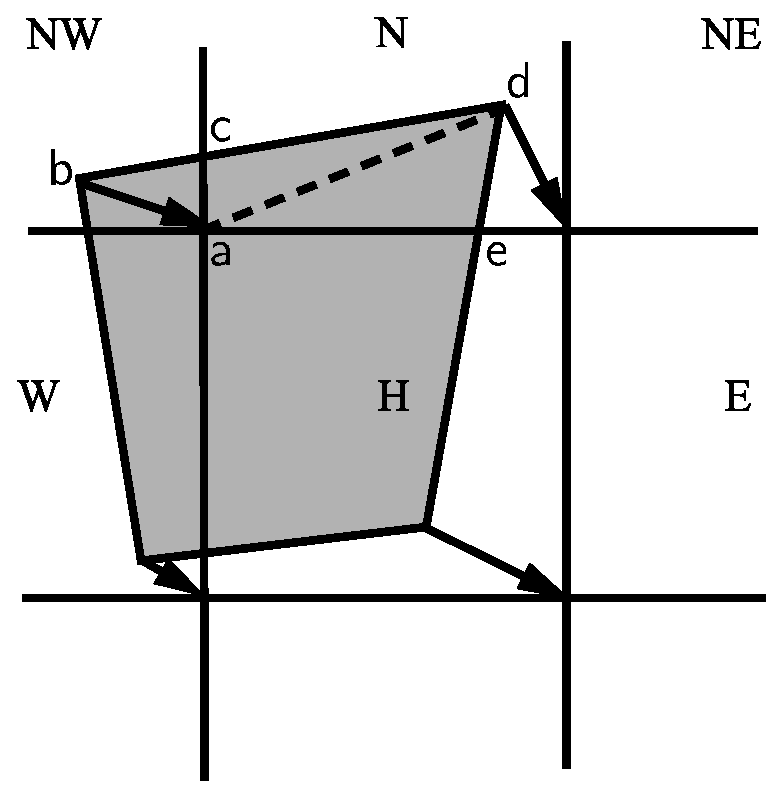
\includegraphics[width=0.5\columnwidth]{\dir/figs/deparr.eps}
  \end{center}
  \caption{In incremental remapping, conserved
    quantities are remapped from the shaded departure region, a
    quadrilateral formed by connecting the backward trajectories
    from the four cell corners, to the grid cell labeled $H$.
    The region fluxed across the north edge of cell $H$ consists
    of a triangle ($abc$) in the $NW$ cell and a quadrilateral 
    (two triangles, $acd$ and $ade$) in the $N$ cell.}
  \label{fig:gliss.deparr}
\end{figure}

Figure~\ref{fig:gliss.triangles}, reproduced from \citet{Dukowicz2000}, shows all possible
triangles that can contribute fluxes across the north edge of a
grid cell.  There are 20 triangles, which can be organized into
five groups of four mutually exclusive triangles as shown in
Table~\ref{table:triangles}. In this table, $(x_1, y_1)$ and $(x_2,y_2)$ are the
Cartesian coordinates of the departure points relative to the
northwest and northeast cell corners, respectively.  The departure
points are joined by a straight line that intersects the west edge
at $(0,y_a)$ relative to the northwest corner and intersects the
east edge at $(0,y_b)$ relative to the northeast corner. The east cell
triangles and selecting conditions are identical except for a
rotation through 90 degrees.

\begin{figure}
  \label{fig:gliss.triangles}
  \centering
    \includegraphics[width=0.7\columnwidth]{\dir/figs/triangles.eps}
  \caption{The 20 possible triangles that can
    contribute fluxes across the north edge of a grid cell.}
\end{figure}


%\newpage
\begin{table}
\begin{center}
\begin{tabular}{cccc}
\hline
Triangle  &  Triangle  &   Selecting logical                   \\
group     &   label    &   condition                           \\
\hline
          &        &            &                                       \\
1         &    NW      &  $y_a>0$ and $y_1\geq0$ and $x_1<0$ \\
          &    NW1     &  $y_a<0$ and $y_1\geq0$ and $x_1<0$ \\
          &    W       &  $y_a<0$ and $y_1<0$ and $x_1<0$    \\
          &    W2      &  $y_a>0$ and $y_1<0$ and $x_1<0$    \\
          &            &                                       \\
2         &    NE      &  $y_b>0$ and $y_2\geq0$ and $x_2>0$    \\
          &    NE1     &  $y_b<0$ and $y_2\geq0$ and $x_2>0$    \\
          &    E       &  $y_b<0$ and $y_2<0$ and $x_2>0$    \\
          &    E2      &  $y_b>0$ and $y_2<0$ and $x_2>0$    \\
          &            &                                       \\
3         &    W1      &  $y_a<0$ and $y_1\geq0$ and $x_1<0$ \\
          &    NW2     &  $y_a>0$ and $y_1<0$ and $x_1<0$    \\
          &    E1      &  $y_b<0$ and $y_2\geq0$ and $x_2>0$ \\
          &    NE2     &  $y_b>0$ and $y_2<0$ and $x_2>0$    \\
          &            &                                       \\
4         &    H1a     &  $y_a y_b\geq 0$ and $y_a+y_b<0$      \\
          &    N1a     &  $y_a y_b\geq 0$ and $y_a+y_b>0$      \\
          &    H1b     &  $y_a y_b<0$ and $\tilde{y}_1<0$      \\
          &    N1b     &  $y_a y_b<0$ and $\tilde{y}_1>0$      \\
          &            &                                       \\
5         &    H2a     &  $y_a y_b\geq 0$ and $y_a+y_b<0$      \\
          &    N2a     &  $y_a y_b\geq 0$ and $y_a+y_b>0$      \\
          &    H2b     &  $y_a y_b<0$ and $\tilde{y}_2<0$      \\
          &    N2b     &  $y_a y_b<0$ and $\tilde{y}_2>0$      \\
          &            &                                       \\
\hline
\end{tabular}
\caption{\label{table:triangles} Evaluation of contributions from the 20 triangles across
the north cell edge.  The coordinates $x_1$, $x_2$, $y_1$, $y_2$,
$y_a$, and $y_b$ are defined in the text. We define $\tilde{y}_1 =
y_1$ if $x_1>0$, else $\tilde{y}_1 = y_a$. Similarly, $\tilde{y}_2
= y_2$ if $x_2<0$, else $\tilde{y}_2 = y_b$.}
\end{center}
\end{table}

Departure triangles across a given cell edge are computed in a local coordinate system whose origin 
lies at the midpoint of the edge and whose vertices are at (-0.5, 0) and (0.5, 0).  
Intersection points are computed assuming Cartesian geometry with cell edges meeting at right angles.  
Let CL and CR denote the left and right vertices, which are joined by line CLR.   
Similarly, let DL and DR denote the departure points, which are joined by line DLR.  
Also, let IL and IR denote the intersection points (0, $y_a$) and (0,$y_b$) respectively, and 
let IC = ($x_c$, 0) denote the intersection of CLR and DLR.  
It can be shown that $y_a$, $y_b$, and $x_c$ are given by

\begin{equation}
  \begin{aligned}
    y_a &=& \frac {{x_{CL} (y_{DM}-y_{DL}) + x_{DM}y_{DL} - x_{DL}y_{DM}}} {x_{DM} - x_{DL}}, \\
    y_b &=& \frac {{x_{CR} (y_{DR}-y_{DM}) - x_{DM}y_{DR} + x_{DR}y_{DM}}} {x_{DR} - x_{DM}}, \\
    x_c &=& (x_{DL} - y_{DL}) \frac{(x_{DR} - x_{DL})} {(y_{DR} - y_{DL})}.
  \end{aligned}
\end{equation}
Each departure triangle is defined by three of the seven points (CL, CR, DL, DR, IL, IR, IC).

Given a 2D velocity field {\bf u}, the divergence $\nabla\cdot{\bf u}$  
in a given grid cell can be computed from the local velocities and written in terms of fluxes across each cell edge:
\begin{equation}
  \label{gliss.eq.IR_divergence}
  \nabla\cdot{\bf u} = \frac{1}{A} 
  \left[\left(\frac{u_{NE}+u_{SE}}{2}\right)L_E + \left(\frac{u_{NW}+u_{SW}}{2}\right)L_W + 
        \left(\frac{u_{NE}+u_{NW}}{2}\right)L_N + \left(\frac{u_{SE}+u_{SW}}{2}\right)L_S \right],
\end{equation}

\noindent
where $L$ is an edge length and the indices $N, S, E, W$ denote compass directions.  
In general, the fluxes in Eq. \eqref{gliss.eq.IR_divergence} are not equal to those implied by the above scheme for locating departure regions.  
For some applications it may be desirable to prescribe the divergence by prescribing the area of the departure region for each edge.  
This can be done by setting {\tt prescribed\_area  = .true.} in {\bf glissade\_transport.F90} and passing the prescribed departure areas 
({\tt edgearea\_e} and {\tt edgearea\_n}) into the remapping routine.  
An extra triangle is then constructed for each departure region to ensure that the total area is equal to the prescribed value.  
This scheme has been used in CICE, but not yet tested in CISM.

In \citet{Dukowicz2000}, departure points are defined by projecting cell
corner velocities directly backward.  That is,
\begin{equation}
  \label{gliss.eq.IR_departure_points} 
  \mathbf{x_D} = -\mathbf{u} \, \Delta t,
\end{equation}
where $\mathbf{x}_D$ is the location of the departure point
relative to the cell corner and $\mathbf{u}$ is the velocity at the corner. 
This approximation is only first-order accurate. Accuracy can be improved by estimating the 
velocity at the midpoint of the trajectory; this is the default in CISM.
(\textbf{Change the default in the code.})

%%%%%%%%%%%%%%%%%%%%%%%%%%%%%%%%%%%%%%%%%%%%%%
\subsubsection{Integrating fields}
\label{sc:glissade-IR-integrate}

Next, we integrate the reconstructed fields over the departure
triangles to find the total volume and internal energy transported
across each cell edge.  Volume transports are easy to compute since the
area is linear in $x$ and $y$.  Given a triangle with vertices
$\mathbf{x_i} = (x_i,y_i)$, $i\in\{1,2,3\}$, the triangle area is

\begin{equation}
  A_T = \frac{1}{2}\left|(x_2-x_1)(y_3-y_1) - (y_2-y_1)(x_3-x_1)\right|.
\end{equation}

\noindent
The integral $F_a$ of any linear function $f(\mathbf{r})$ over a triangle is given by

\begin{equation}
  \label{gliss.eq.IR_integrate1}
  F_a = A_T f(\mathbf{x_0}),
\end{equation}
where $\mathbf{x}_0 = (x_0,y_0)$ is the triangle midpoint,
\begin{equation}
  \mathbf{x}_0 = \frac{1}{3} \sum_{i=1}^3\mathbf{x}_i.
\end{equation}
To compute the thickness transport, we evaluate the thickness at the midpoint,
\begin{equation}
  a(\mathbf{x}_0)  = a_c + a_x x_0 + a_y y_0,
\end{equation}
and multiply by $A_T$.  By convention, northward and eastward
transport is positive, while southward and westward transport is
negative.

Eq. \eqref{gliss.eq.IR_integrate2} cannot be used for energy transport, because
the reconstructed internal energy is a quadratic function of position.
(It is the product of two linear functions, for thickness and temperature.)
The integral of a quadratic polynomial over a triangle requires
function evaluations at three points,
\begin{equation}
  \label{gliss.eq.IR_integrate2}
  F_h = \frac{A_T}{3}\sum_{i=1}^3 f\left({\mathbf x}^\prime_i\right),
\end{equation}
where $\mathbf{x}_i^\prime = (\mathbf{x}_0+\mathbf{x}_i)/2$ are
points lying halfway between the midpoint and the three vertices.

%%%%%%%%%%%%%%%%%%%%%%%%%%%%%%%%%%%%%%%%%%%%%%
\subsubsection{Updating state variables}
\label{sc:glissade-IR-update}

Finally, we compute new values of the state variables in each ice layer of each grid cell.
The new ice thickness $H^\prime(i,j)$ is given by
\begin{equation}
  \label{gliss.eq.IR_new_area}
  H^\prime(i,j) = H(i,j) + 
  \frac{F_{E}(i-1,j) - F_{E}(i,j) + F_{N}(i,j-1) - F_{N}(i,j)} {A(i,j)}
\end{equation}
where $F_{E}(i,j)$ and $F_{N}(i,j)$ are the volume transports across the
east and north edges, respectively, of cell $(i,j)$, and $A(i,j)$
is the grid cell area.   All transports added to one cell are
subtracted from a neighboring cell; thus \eqref{gliss.eq.IR_new_area}
conserves total ice volume.

The new internal energy in each layer is computed analogously.
New temperatures are then given by the ratio of energy to volume
(and other tracers, if present, are updated in the same way).
Tracer monotonicity is ensured because
\[ T^\prime = \frac{\int_A H \, T \, dA} {\int_A H \, dA}, \]
where $T^\prime$ is the new-time temperature, given by 
integrating the old-time thickness and temperature
over a Lagrangian departure region with area $A$. That is,
the new-time temperature is a weighted averages over
old-time values, with non-negative weight $H$. Thus the
new-time values must lie between the maximum and minimum of the
old-time values.

%%%%%%%%%%%%%%%%%%%%%%%%%%%%%%%%%%%%%%%%%%%%%%
\subsubsection{CFL checks}
\label{sc:glissade-IR-CFL}

As mentioned above, the time step used for explicit advection is limited by an
advective CFL (Courant--Friedrichs--Lewy) condition (Eq. \ref{eq:CFL}).  
Furthermore, for ice flux parallel to $\nabla s$, ice thickness evolution is diffusive,
rising to an additional diffusive CFL condition \citep{Bueler:2009ee}:
\begin{equation}
    \frac{\max D \Delta t} { {\Delta x}^\frac{1}{2}} \leq 2 
\end{equation}
Flow governed by the Shallow Ice Approximation is always subject to this diffusive CFL,
but some component of higher-order flow may not be because some component of the ice
velocity may not be parallel to $\nabla s$ \citep{Bueler:2009ee}.

For these reasons, Glissade's transport scheme performs a check of both the
advective and diffusive CFL conditions and writes a warning to the log file if
either of them is violated.  These warnings indicate the $i,j$ indices (on the global domain)
of where the worst violation occurred, as well as the maximum allowable time step
given the CFL condition(s).

The diffusivity is approximated using the component of velocity in the downslope
direction:
\begin{equation}
  D = \frac{(\vec{u} \cdot \nabla h) H}{|\nabla h|}
\end{equation}
Future work may identify a less restrictive diffusivity, so the diffusive CFL 
warnings currently written may be overly restrictive.  In other words, you may see
stable model results that generate a diffusive CFL warning.  

Advective CFL violations generally lead to stability problems with 
thickness evolution.  However, since CFL violations may occur in portions of the
domain that are not of interest to the user, these situations are not set to be
a fatal error.  Note, however, that the Incremental Remapping scheme may encounter
a `departure points out of bounds' error when advective CFL violations occur, and this is a
failure in the method that does result in a fatal error.

Eventually, CISM may include an adaptive time stepping scheme that adjusts the 
model time step based on the advective and diffusive CFL conditions.  However, 
at present, the time step must be set manually and remain constant over a simulation.
To aid in determining an appropriate time step for a simulation, the \texttt{adv\_cfl\_dt}
and \texttt{diff\_cfl\_dt} variables can be added to an output file.  These variables
write the maximum allowable time step at each time in the model based on the 
advective and diffusive CFL conditions, respectively.  Note that in some cases 
stability may only be achieved by taking half of the reported values.





\section{Temperature solver}
\label{sc:glissade-temperature}

Some text here



%\chapter{Physics}
%\renewcommand{\dir}{physics}
%\input{\dir/subglacial-hydrology.tex}
\input{\dir/calving.tex}
\input{\dir/basal-processes.tex}


\chapter{Running CISM}
\renewcommand{\dir}{run_cism}
\label{ch:runcism}

\section{Overview of Running CISM}

Assuming you successfully completed the Installation instructions in Chapter \ref{chp:install},
the executable for running the model, \texttt{cism\_driver}, can be found in your 
build directory in a subdirectory called \texttt{cism\_driver} 
(e.g., \texttt{./builds/mac-gnu/cism\_driver/cism\_driver}).

The build system creates the executable at this path but does not automatically
make it available to other locations on your system.  How you choose to do so depends 
on your situation.  See the introduction to Chapter \ref{chp:testcases} for 
an overview of how to make the executable available to other locations on your system
(e.g., symlinking, copying, or modifying your PATH environment variable).

Unlike previous versions of Glimmer, with CISM 2.0 this single \texttt{cism\_driver} 
executable is used for running the model in all configurations.
\texttt{cism\_driver} can be invoked with a single argument specifying 
a CISM .config file to run CISM as a standalone ice sheet model without Glint climate forcing,
or with two arguments (a CISM config file and a Glint config file) 
to run CISM with Glint climate forcing:
\begin{verbatim}
 Call cism_driver with either 1 or 2 arguments. Examples:
 cism_driver ice_sheet.config
 cism_driver ice_sheet.config climate.config
\end{verbatim}
The available options for the CISM configuration file and 
for the Glint climate interface configuration file are described in detail below.

To perform a parallel run with the parallel build of CISM, you must use the
MPI run command, which is typically \texttt{mpirun} or \texttt{mpiexec} but may 
vary among MPI versions and installations.  A standard syntax that is likely to
work on most installations is \newline
 \indent \texttt{mpirun -np N cism\_driver ice\_sheet.config \textit{climate.config}} \newline
where \texttt{N} is the number of processors you want to use, \texttt{ice\_sheet.config} is the name of the CISM
configuration file, and the optional argument \texttt{\textit{climate.config}} is the name 
of the climate configuration file.  For example: \newline
 \indent \texttt{mpirun -np 4 cism\_driver dome.config}\newline
would run the dome test case on four processors.

Finally, note that instructions for running CISM within the Community Earth System Model (CESM)
or another climate model are not described here.

When CISM runs, some basic information about its operation will be output to 
the screen (standard out).  More verbose information about the run will be written 
to a log file which is named \texttt{\textit{ice\_sheet.config}.log} where 
\texttt{\textit{ice\_sheet.config}} is the name of the .config file use to perform
the run.  (For example, if running the model with  \texttt{./cism\_driver dome.config},
the log file will be called  \texttt{dome.config.log}.)  The log file is an
important reference, especially for debugging runs that do not behave as expected.
For example, the log file includes a list of configuration options and parameter
values, which can be useful in diagnosing problems like typos in your .config file.
The log file also indicates what files were used for input and output and at which
times I/O occurred.  The log file may contain warnings about potentially
problematic configuration combinations or model behavior, such as the use of
configurations settings that are not scientifically validated, or a CFL violation
during advection.  In contrast, fatal errors will kill the model and the error
message will be written to both the screen and the log file.

Optionally, the log file also contains diagnostic information about the global
state of the ice sheet (e.g., the total ice area and volume, the maximum surface and basal
speeds, and the max and min temperatures), along with vertical profiles of speed
and temperature at a user-specified grid point.  This information is written at intervals
specified by the config file variable \texttt{dt\_diag}, for the diagnostic
point \texttt{(idiag,jdiag)}.

In addition to the log file, the model will create any netCDF output files requested
in the config file (see Section \ref{io-config} below for details).  
If the model dies for some reason midway through a simulation,
the netCDF files will still include output for the portion of the simulation that 
was completed.

\section{Overview of Configuration Files}

Running CISM is managed through configuration files (*.config) that enable 
desired model features and control input of initial conditions and forcing 
and output of model results.  This chapter summarizes the configuration options 
available for running CISM and is divided into sections on general Model Configuration, 
Input/Ouput Configuration, and optional Climate Forcing Configuration.

The format of CISM configuration files is taken from that used by the 
ConfigParser module in Python 2.x, which is similar to Windows \texttt{.ini} files 
and contains sections. Each section contains key/value pairs.

\begin{itemize}
\item[Comments:] Empty lines, or lines starting with a \texttt{\#}, \texttt{;} or \texttt{!} are ignored.  Comments can also be added on the same line as a key/value pair using these delimiters.
\item[Sections:] A new section starts with the section name enclosed by square brackets, \texttt{[ ]} and can be up to 50 characters long, e.g., \texttt{[grid]}.
\item[Key/Value Pairs:] Keys are separated from their associated values by \texttt{=} or \texttt{:}. The names can be up to 50 characters long. Values can be up to 400 characters long.
\end{itemize}

Sections and keys are case-sensitive and may contain white space. 
However, the configuration parser is very simple and thus the number of spaces 
within a key or section name also matters. Sensible defaults are used when 
a specific key is not found; defaults are shown in bold in the tables below.

Here is an example configuration file:
\begin{verbatim}
;a comment
[a section]
an_int  : 1
a_float = 2.0
a_char  = hey, this is rather cool
an_array = 10. 20. -10. 40. 100.

[another section]
! more comments
foo : bar
\end{verbatim}




\section{Model Configuration}\label{ug.sec.config}

General model configuration options 
specify the grid and time-stepping used by the model, 
the dynamical core (dycore) used, 
and control various optional physics packages and parameter values.
The \texttt{[grid]} and \texttt{[time]} configuration sections are always required.
Also, while not required, in almost all situations  \texttt{[options]} 
and (if using a higher-order dycore) \texttt{[ho\_options]} will be included in .config files.
The \texttt{[parameters]} and \texttt{[sigma]} sections are also commonly used.  
The \texttt{[GTHF]}, \texttt{[isostasy]}, and \texttt{[projection]} sections
are needed only if the associated features are desired.  Details of each of these
sections, what they control, and the available options for each section are listed 
in the tables below.

\begin{center}
  \tablefirsthead{%
    \hline
  }
  \tablehead{%
    \hline
    \multicolumn{2}{|l|}{\emph{\small continued from previous page}}\\
    \hline
  }
  \tabletail{%
    \hline
    \multicolumn{2}{|r|}{\emph{\small continued on next page}}\\
    \hline}
  \tablelasttail{\hline}
  \begin{supertabular*}{\textwidth}{@{\extracolsep{\fill}}|l|p{10cm}|}


%%%% GRID
    \hline
    \multicolumn{2}{|l|}{\texttt{[grid]}}\\
    \hline
    \multicolumn{2}{|p{0.97\textwidth}|}{Define model grid. 
%Maybe we should make this optional and read grid specifications from input netCDF file (if present). Certainly, the input netCDF files should be checked (but presently are not) if grid specifications are compatible.
}\\
    \hline
    \texttt{ewn} & (integer) number of nodes in $x$--direction\\
    \texttt{nsn} & (integer) number of nodes in $y$--direction\\
    \texttt{upn} & (integer) number of nodes in $z$--direction\\
    \texttt{dew} & (real) node spacing in $x$--direction (m)\\
    \texttt{dns} & (real) node spacing in $y$--direction (m)\\
%% global_bc
    \texttt{global\_bc} & 
        boundary conditions for the edges of the global domain \\ &
    \begin{tabular}[t]{cp{0.85\linewidth}}
      {\bf 0} & periodic \\
      1 & outflow \\
    \end{tabular}\\
%    \texttt{sigma\_file} & (string) Name of file containing $\sigma$ coordinates. Alternatively, the sigma levels may be specified using the \texttt{[sigma]} section decribed below. If no sigma coordinates are specified explicitly, they are calculated based on the value of \texttt{sigma\_builtin} \\
    \texttt{sigma} &
%    \begin{tabular}[t]{cp{\linewidth}}
%      \multicolumn{2}{p{0.72\textwidth}}{If sigma coordinates are not specified in this configuration file or using the \texttt{sigma\_file} option, this specifies how to compute the sigma coordinates.} \\
      method for specifying sigma coordinates:  \\ &
    \begin{tabular}[t]{cl}
      {\bf 0} & Use Glimmer's default spacing \\[0.05in] 
        & $\sigma_i=\frac{1-(x_i+1)^{-n}}{1-2^{-n}}\quad\mbox{with}\quad x_i=\frac{\sigma_i-1}{\sigma_n-1}, n=2.$ \\[0.05in]
      1 & use sigma coordinates defined in external file (named sigma\_file) \\
      2 & use sigma coordinates given in configuration file \\
      3 & use evenly spaced sigma levels (required by the Glam dycore) \\
      4 & use Pattyn sigma levels \\
    \end{tabular}\\



%%%% SIGMA
    \hline
    \hline
    \hline
    \multicolumn{2}{|l|}{\texttt{[sigma]}}\\
    \hline
    \multicolumn{2}{|p{0.95\textwidth}|}{Define the sigma levels used in the vertical discretization (\texttt{sigma}=2 above). This is an alternative to using a separate file (specified in section \texttt{[grid]} above). If neither is used, the levels are calculated as described above.} \\
    \hline
    \texttt{sigma\_levels} & (real) list of sigma levels, in ascending order, separated by spaces. These run between 0.0 and 1.0. \\



%%%% TIME
    \hline
    \hline
    \hline
    \multicolumn{2}{|l|}{\texttt{[time]}}\\
    \hline
    \multicolumn{2}{|p{0.95\textwidth}|}{Configure time steps diagnostic specifications} \\
    %{\bf TODO: address / remove this next note:} Update intervals should probably become absolute values rather than related to the main time step when we introduce variable time steps. \textbf{Steve: I don't actually know what the question is here or what this note is supposed to be about.}}\\
    \hline
    \texttt{tstart} & (real) start time of the model in years\\
    \texttt{tend} & (real) end time of the model in years\\
    \texttt{dt} & (real) size of time step in years\\
    \texttt{subcyc} & (integer) number of time steps to subcycle within dt using a steady velocity field \\
    \texttt{ntem} & (real) time step multiplier setting the ice temperature update interval\\
%    \texttt{nvel} & (real) time step multiplier setting the velocity update interval\\
%    \texttt{profile} & (integer) profile frequency (number of time steps) {\bf TODO: more useful description of what profiling is? Steve: I've never used this either.   
%    Matt, my guess would be that Pat's profiling code is superior to this and, if we document that anywhere (do we?), we should support using that instead.}\\
%   Matt: Disabling this for 2.0 release
    \texttt{dt\_diag} & (real) writing diagnostic variables to log file every dt\_diag yrs\\
    \texttt{idiag} & (int) $x$ direction index for diagnostic grid point in log file\\
    \texttt{jdiag} & (int) $x$ direction index for diagnostic grid point in log file\\
%    \texttt{ndiag} & (int) number of time steps between diagnostics. {\bf DEPRECATED}.  Use \texttt{dt\_diag}. \textbf{Steve: Should we then remove and replace this with dt\_diag rather than using the old var name?}\\



%%%% Options
    \hline
    \hline
    \hline
    \multicolumn{2}{|l|}{\texttt{[options]}}\\
    \hline
    \multicolumn{2}{|p{0.95\textwidth}|}{Parameters set in this section determine how various components of the ice sheet model are treated.  Configuration number options with a $\dagger$ are specific to the higher-order dycores (e.g., Glissade). Options with a ? are working, but are currently not scientifically supported, and are therefore for use at your own risk. Options with a ! are in development and will be supported in future code releases. }\\
    \hline
%% dycore
    \texttt{dycore} & 
    \begin{tabular}[t]{lp{0.85\linewidth}}
      0 & Glide (1-processor, 3d, shallow-ice-approximation dycore) \\
      1$\dagger$? & Glam (parallel, 3d, FDM, 1st-order-accurate dycore)  \\
      {\bf 2$\dagger$} & Glissade (parallel, 3d, FEM, 1st-order-accurate dycore)  \\
      3$\dagger$! & FELIX (parallel, 3d, FEM, 1st-order-accurate dycore)  \\
      4$\dagger$! & BISICLES (parallel, quasi-3d, FVM, L1L2 dycore)  \\
    \end{tabular}\\
%% evolution
    \texttt{evolution} (ice thickness) & 
    \begin{tabular}[t]{lp{0.85\linewidth}}
      {\bf 0} & pseudo-diffusion (Glide only)\\
      1 & ADI scheme  (Glide only)\\
      2 & diffusion (Glide only)\\
      3$\dagger$ & incremental remapping \\
      4$\dagger$ & first-order upwind  \\
      5$\dagger$ & evolve without changing ice thickness (Useful for running with a fixed geometry, e.g. for a temperature spinup. On each time step, geometry and tracers are evolved using incremental remapping, after which geometry is reset to its initial value. This evolution scheme is still subject to the advective CFL condition.)\\
    \end{tabular}\\
%% temperature
    \texttt{temperature} & 
    \begin{tabular}[t]{lp{0.85\linewidth}}
      0 & Set each ice column to local surface air temperature \\
      {\bf 1} & prognostic temperature calculation \\
      2 & hold temperature steady at initial value \\
      3! & prognostic temperature calculation using enthalpy-based formulation \\
    \end{tabular}\\
%% temperature init
    \texttt{temp\_init} & 
    \begin{tabular}[t]{lp{0.85\linewidth}}
      0 & initial temperatures isothermal at $0^\circ$C\\
      {\bf 1} & initial column temperatures set to atmos. temperature \\
      2 & initial column temperatures linearly interpolated between atmos. temperature and pressure melting point\\
    \end{tabular}\\
%% flow law
    \texttt{flow\_law} &  
    \begin{tabular}[t]{lp{0.85\linewidth}}
      {\bf 0}  & constant (using the value of \texttt{default\_flwa)}\\
      1 & temperature-dependent, \citet{PatersonBudd:1982} ($T=-5^\circ$C)\\
      2 & temperature-dependent, \citet{PatersonBudd:1982} (function of variable T)\\
    \end{tabular}\\
%% basal water
    \texttt{basal\_water} & 
    \begin{tabular}[t]{lp{0.85\linewidth}}
      {\bf 0} & none \\
      1 & local water balance\\
      2 & compute the steady-state, routing-based, basal water flux and water layer thickness (NOTE: not supported for $> 1$ processor) \\
      3 & use a constant basal water layer thickness everywhere, to enforce T=T${_{pmp}}$ everywhere \\
      4! & ocean penetration parameterization for effective pressure from \citet{Leguy2014} \\
    \end{tabular}\\
%% basal mass balance
    \texttt{basal\_mass\_balance} & 
    \begin{tabular}[t]{lp{0.85\linewidth}}
      {\bf 0} & ignore basal melt rate in mass balance calculation \\
      1 & include basal melt rate in mass balance calculation \\
    \end{tabular}\\
%% slip coefficient
    \texttt{slip\_coeff} & 
        slip coefficient (Glissade local SIA and Glide \textit{only}) \\ &
    \begin{tabular}[t]{lp{0.85\linewidth}}
      {\bf 0} & zero (no sliding) \\
      1 & set to a non--zero constant everywhere\\
      2 & set to constant where basal water (bwat) is nonzero\\
      3 & set to constant where the ice base is melting\\
      4 & set proportional to basal melt rate\\
      5 & \texttt{tanh} function of basal water (bwat)\\
    \end{tabular}\\
%% marine margin
    \texttt{marine\_margin} & 
    \begin{tabular}[t]{lp{0.85\linewidth}}
      0 & ignore marine margin\\
      {\bf 1} & set thickness to zero if floating\\
      2 & lose fraction of ice from edge cells\\
      3 & set thickness to zero if relaxed bedrock is below a given depth (variable ``mlimit" in glide\_types)\\
      4 & set thickness to zero if present-day bedrock is below a given depth (variable ``mlimit" in glide\_types)\\
      5? & Huybrechts calving scheme \\
    \end{tabular}\\
%% vertical integration
    \texttt{vertical\_integration} & 
       (Glide \textit{only}) \\ &
    \begin{tabular}[t]{lp{0.85\linewidth}}
      {\bf 0} & standard integration (to obtain vertical velocity profile)\\
      1 & constrained to obey kinematic velocity at upper surface boundary\\
    \end{tabular}\\
%% geothermal heat flux
    \texttt{gthf} &  
    \begin{tabular}[t]{lp{0.85\linewidth}}
      {\bf 0} & prescribed, uniform geothermal heat flux \\
      1 & read 2d geothermal heat flux field from input file \\
      2 & calculate geothermal heat flux using 3d diffusion model \\
    \end{tabular}\\
%% isostasy
    \texttt{isostasy} &  
    \begin{tabular}[t]{lp{0.85\linewidth}}
      {\bf 0} & no isostatic adjustment \\
      1 & compute isostatic adjustment using lithosphere / asthenosphere model (see below for available options)  \\
    \end{tabular}\\
%% topography
    \texttt{topo\_is\_relaxed} &  
    \begin{tabular}[t]{lp{0.85\linewidth}}
      {\bf 0} & relaxed topography is read from a separate input variable, \texttt{relx} \\
      1 & first time slice of input topography is assumed to be relaxed\\
      2 & first time slice of input topography is assumed to be in isostatic
      equilibrium with ice thickness \\
    \end{tabular}\\
%% periodicity					%% no longer used / supported
%    \texttt{periodic\_ew} & 
%  {\bf TODO: Is this still used?  If so, do we need to add perdiodic\_ns?} \\&
%    \begin{tabular}[t]{lp{0.85\linewidth}}
 %     {\bf 0} & switched off\\
 %     1 & periodic lateral EW boundary conditions (Glide  dycore \textit{only}) \\
 %   \end{tabular}\\
%% restart
    \texttt{restart} &
    \textit{Note:} alternate keyword {\bf hotstart} is retained for backwards compatibility. \\ &
    \begin{tabular}[t]{lp{0.85\linewidth}}
      {\bf 0} & normal start (initial values taken from input file or, if absent, using default options)\\
      1 & restart model using input from previous run;
           specific fields required for restart are dependent on chosen options (add ``restart" to the 
           \texttt{variable} list in the \texttt{[CF output]} section of the \texttt{.config} file to automatically save the appropriate restart fields.)\\
    \end{tabular}\\
    \hline
    \texttt{ioparams} & (string) name of file containing netCDF I/O configuration. The main configuration file is searched for I/O related sections if no file name is given (default).  In other words, you can remove sections \texttt{CF input}, \texttt{CF output}, and \texttt{CF forcing} from the primary configuration file and place them in a separate file, the path to which is specified here.\\



 %%%% HIGHER-ORDER OPTIONS
    \hline
    \hline
    \hline
    \multicolumn{2}{|l|}{\texttt{[ho\_options]}}\\
    \hline
    \multicolumn{2}{|p{0.95\textwidth}|}{Options set in this section determine how various components of the higher-order extensions to the ice sheet model (e.g., Glissade) are treated. Defaults are indicated in bold. These options have no effect on the shallow-ice (Glide) dycore. In this section, options with a ? are working but are currently not scientifically supported (and are therefore for use at your own risk). Options marked with a * apply only to a serial build (or a parallel build if run on 1 processor). Options marked with a ! are under development and will be supported in future versions of the code (hence, these are also for use at your own risk).}\\
    \hline
%% which_ho_nonlinear
    \texttt{which\_ho\_nonlinear} & 
    \begin{tabular}[t]{lp{0.85\linewidth}}
      {\bf 0} & treat nonlinearity in momentum balance using Picard iteration \\
      1? & treat nonlinearity in momentum balance using Jacobian-Free Newton-Krylov iteration (Glam only)  \\
    \end{tabular}\\     
%% which_ho_sparse
    \texttt{which\_ho\_sparse} & 
%\\ &
    \begin{tabular}[t]{lp{0.85\linewidth}}
      -1* & solve sparse linear system using SLAP with incomplete Cholesky preconditioned conjugate gradient method\\
      0* & solve sparse linear system using SLAP with incomplete LU-preconditioned biconjugate gradient method\\
      1* & solve sparse linear system using SLAP with incomplete LU-preconditioned GMRES method\\
      2 & solve sparse linear system using preconditioned conjugate gradient method: standard algorithm (Glissade only) \\
      {\bf 3} & solve sparse linear system using preconditioned conjugate gradient method: Chronopoulos-Gear algorithm (Glissade only)\\
      4 & solve sparse linear system using \textit{Trilinos}, incomplete LU-preconditioned GMRES method (\textit{Trilinos}-compatible build only)\\
    \end{tabular}\\     
%% which_ho_efvs
    \texttt{which\_ho\_efvs} & 
    \begin{tabular}[t]{lp{0.85\linewidth}}
      0 & use a constant value for the effective viscosity (i.e., linear viscosity). The default value is 2336041 Pa yr (as used by ISMIP-HOM Test F).\\
      1 & set the effective viscosity to a value based on the flow rate factor: efvs $= 0.5 * A^{-1/n}$\\
      {\bf 2} & use the effective strain rate to compute the effective viscosity (i.e., full nonlinear treatment) \\
    \end{tabular}\\  
%% which_no_disp
    \texttt{which\_ho\_disp} & 
    \begin{tabular}[t]{lp{0.85\linewidth}}
      -1 & no dissipation term included in temperature equation \\
      0 & calculate dissipation in temperature equation assuming SIA ice dynamics \\
      {\bf 1} & calculate dissipation in temperature equation assuming first-order ice dynamics \\
    \end{tabular}\\    
%% which_ho_babc
    \texttt{which\_ho\_babc} & 
        Implementation of basal boundary condition in higher-order dycore \\ &
    \begin{tabular}[t]{lp{0.85\linewidth}}
      0 & constant value of ``beta" \\
      1 & specify a simple pattern for ``beta" (hardcoded, mainly useful for debugging)\\
      2 & read map of yield stress (in Pa) from input field ``mintauf" to simulate sliding 
          over a plastic subglacial till (Picard-based solution) \\
      3 & calculate ``beta" as linear (inverse) function of basal water thickness\\
      {\bf 4} & (virtually) no slip everywhere in domain (``beta" set to very large value)\\
      5 & read map of ``beta" from .nc input file using standard I/O \\
      6 & no slip everywhere in domain (using Dirichlet basal BC)\\
      7! & read map of yield stress (in Pa) from input field ``mintauf" to simulate sliding 
          over a plastic subglacial till (Newton-based solution)\\
      8* & Spatial field of ``beta" required for ISMIP-HOM Test C (avoids interpolation error 
          associated with option 5; works for a single processor only) \\
      9! & Weertman-style power-law accounting for effective pressure (Eq. \ref{weertmansliding2}) \\
      10! & Coulomb friction law (Eq. \ref{CF-law}) \\
    \end{tabular}\\  
%% which_ho_resid
    \texttt{which\_ho\_resid} &
     Residual calculation method for higher-order velocity solvers (e.g., Glissade). 
     Nonlinear iterations are halted once the residual falls below a specified value. \\ &
    \begin{tabular}[t]{lp{0.85\linewidth}}
      0? & use the maximum value of the normalized velocity vector update, defined by 
      $r = \frac{|vel_{k-1} - vel_k|}{vel_k}$ \\
      1? & as in option 0 but omitting the basal velocities from the comparison
          (useful in cases where an approx. no slip basal BC is enforced) \\
      2? & as in option 0 but using the mean rather than the max \\
      {\bf 3} & use the L2 norm of the system residual, defined by $r = Ax - b$ \\
    \end{tabular}\\  
%% which_ho_approx
    \texttt{which\_ho\_approx} &
     Stokes-flow approximation to use with Glissade dycore \\ &
    \begin{tabular}[t]{lp{0.85\linewidth}}
      -1 & local shallow-ice approximation, Glide-type calculation (uses glissade\_velo\_sia) \\
      0 & 3d matrix shallow-ice approximation, vertical-shear stresses only (uses glissade\_velo\_higher) \\
      1 & shallow-shelf approximation (SSA) with horizontal-plane stresses only (uses glissade\_velo\_higher; requires \texttt{which\_ho\_precond} $<=$1) \\
      {\bf 2} & Blatter-Pattyn with both vertical-shear and horizontal-plane stresses (uses glissade\_velo\_higher) \\
       3 & depth-integrated (L1L2) approximation, with both vertical shear and horizontal-plane stresses (uses glissade\_velo\_higher; requires \texttt{which\_ho\_precond} $<=$1) \\
    \end{tabular}\\  
%% which_ho_precond
    \texttt{which\_ho\_precond} &
     Preconditioner to use in the linear PCG solve of the Glissade dycore \\ &
    \begin{tabular}[t]{lp{0.85\linewidth}}
      0 & no preconditioner \\
      1 & diagonal preconditioner \\
      {\bf 2} & physics-based (shallow-ice) preconditioner (not valid for SSA and L1L2) \\
    \end{tabular}\\  
%% which_ho_gradient
    \texttt{which\_ho\_gradient} &
     Which spatial gradient operator to use in the Glissade dycore \\ &
    \begin{tabular}[t]{lp{0.85\linewidth}}
      {\bf 0} & centered gradient \\
      1 & upstream gradient (damps checkerboard noise in prognostic simulations) \\
    \end{tabular}\\  
%% which_ho_gradient_margin
    \texttt{which\_ho\_gradient\_margin} &
     Spatial gradient operator to use in the Glissade dycore at ice sheet margins. \\ &
    \begin{tabular}[t]{lp{0.85\linewidth}}
      0 & use information from all neighboring cells, ice-covered or ice-free \\
      {\bf 1} & use information from ice-covered and/or land cells, but not ice-free ocean cells \\
      2 & use information from ice-covered cells only \\
    \end{tabular}\\  
%% which_ho_assemble_beta
    \texttt{which\_ho\_assemble\_beta} &
     Finite-element assembly method for basal boundary conditions that use ``beta" field \\ &
    \begin{tabular}[t]{lp{0.85\linewidth}}
      {\bf 0} & Standard finite-element calculation, which effectively applies a smoothing to ``beta" (and ``mintauf") \\
      1 &  Apply the local ``beta" (or ``mintauf") value at each vertex (no smoothing) \\ 
    \end{tabular}\\  
%% glissade_maxiter
    \texttt{glissade\_maxiter} &
    \begin{tabular}[t]{lp{0.85\linewidth}}
	{\bf 100} & Maximum number of nonlinear (Picard) iterations in the Glissade dycore \\ 
    \end{tabular}\\  



% MJH: Commenting out external dycore options for 2.0 release.
%% %%%% EXTERNAL DYCORE OPTIONS
%    \hline
%    \hline
%    \hline
%    \multicolumn{2}{|l|}{\texttt{[external\_dycore\_options]}}\\
%    \hline
%    \multicolumn{2}{|p{0.95\textwidth}|}{Options set in this section are specific to external dycores that 
%    may have additional options/option files.  {\bf TODO: include this stuff?  elaborate?} }\\
%    \hline
%%% external_dycore_type
%    \texttt{external\_dycore\_type} & 
%    \begin{tabular}[t]{lp{0.85\linewidth}}
%      1 & Use BISICLES external dycore \\
%      2 & Use Albany-FELIX external dycore \\
%    \end{tabular}\\     
%    \texttt{dycore\_input\_file} &
%    Specify path to additional configuration file required by the external dycore. \\



%%%% PARAMETERS
    \hline
    \hline
    \hline
    \multicolumn{2}{|l|}{\texttt{[parameters]}}\\
    \hline
    \multicolumn{2}{|p{0.95\textwidth}|}{Set values for various parameters.  Parameters with a $\dagger$ are specific to the higher-order dycores (e.g., Glissade).}\\
    \hline
    \texttt{log\_level} & (integer) set to a value between 0, no messages, and 6, all messages are displayed to stdout. By default, messages are only logged to a file.
    The format for this filename is ``configuration-file-name.config.log" \\
    \texttt{ice\_limit} & (real) below this limit ice is only accumulated/ablated; ice dynamics are switched on once the ice thickness is above this value. (default = 100.0 m) \\
    \texttt{ice\_limit\_temp} $\dagger$ & (real) minimum thickness for computing vertical temperature (m). (default = 1.0 m) \\
    \texttt{marine\_limit} & (real) all ice is assumed lost (calved) once water depths reach this value (for \texttt{marine\_margin}=3 or 4 in 
    \texttt{[options]} above). Note, water depth is negative.  (default = -200.0 m) \\
    \texttt{calving\_fraction} & (real) fraction of ice lost due to calving (for \texttt{marine\_margin}=2). (default = 0.8)\\
    \texttt{geothermal} & (real) constant geothermal heat flux, positive down by convention (hence < 0). (default = -0.05 W m$^{-2}$)\\
    \texttt{flow\_factor} & (real) the flow law rate factor is multiplied by this factor (default = 1.0; in previous versions of Glimmer-CISM the default value was 3.0) \\
    \texttt{default\_flwa} & flow law parameter A to use in isothermal experiments (flow\_law set to 0).  Default value is $10^{-16}$ Pa$^{-n}$ yr$^{-1}$. This 
    overrides any temperature dependence. \\
    \texttt{efvs\_constant} $\dagger$ & Constant value of effective viscosity when using \texttt{which\_ho\_efvs}=0. Default value is 2336041 Pa yr, as in ISMIP-HOM Test F. \\
%    \texttt{hydro\_time} & (real) basal hydrology time constant (default = 1000.0 yr) {\bf TODO: IS THIS STILL USED? Steve: I grepped for it in a few different dirs. The only place
%    I saw it was in glide setup, suggesting that it is not being used right now.}\\
    \texttt{basal\_tract\_const} & constant basal traction parameter. You can load a .nc file with a variable called \texttt{soft} if you want a spatially varying 
    bed softness parameter (Glissade local SIA and Glide only) \\
    \texttt{basal\_tract\_max} & max value for basal traction when using \texttt{slip\_coeff}=4. \\
    \texttt{basal\_tract\_slope} & slope value for basal traction relation when using \texttt{slip\_coeff}=4. (Relation also uses \texttt{basal\_tract\_const}.)\\
    \texttt{basal\_tract\_tanh} & (real(5)) basal traction factors. Basal traction is set to $B=\tanh(W)$ with the parameters
      \begin{tabular}{cp{\linewidth}}
       (1) & width of the $\tanh$ curve\\
       (2) & $W$ at midpoint of $\tanh$ curve [m]\\
       (3) & $B$ minimum [ma$^{-1}$Pa$^{-1}$] \\
       (4) & $B$ maximum [ma$^{-1}$Pa$^{-1}$] \\
       (5) & multiplier for marine sediments \\
     \end{tabular}\\
    \texttt{ho\_beta\_const} $\dagger$ & (real) spatially uniform beta used when \texttt{which\_ho\_babc} = 0. (default = 10.0 Pa yr m$^{-1}$) \\
    \texttt{friction\_powerlaw\_k} $\dagger$ & (real) friction coefficient $k$ used for \texttt{which\_ho\_babc} = 9 (Eq. \ref{weertmansliding2}) (default = 8.4e-9 m y$^{-1}$ Pa$^{-2}$, from \citet{Bindschadler1983} converted to CISM units) \\
    \texttt{coulomb\_c} $\dagger$ & (real) Coulomb friction coefficient (unitless), $C$,
used for \texttt{which\_ho\_babc} = 10 (Eq. \ref{CF-law}) (default = 0.42, from \citet{Pimentel2010a}) \\
    \texttt{coulomb\_bump\_wavelength} $\dagger$ & (real) wavelength (m) of the dominant bedrock bumps, $\lambda_{max}$,
used for \texttt{which\_ho\_babc} = 10 (Eq. \ref{CF-law}) (default = 2.0 m, from \citet{Pimentel2010a}) \\
    \texttt{coulomb\_bump\_slope} $\dagger$ & (real) maximum slope (unitless) of the dominant bedrock bumps, $m_{max}$,
used for \texttt{which\_ho\_babc} = 10 (Eq. \ref{CF-law}) (default = 0.5 m, from \citet{Pimentel2010a}) \\
    \texttt{p\_ocean\_penetration} & (real) $p$-exponent in ocean penetration parameterization for (\texttt{basal\_water} = 4 (default = 0.0)\\
    \texttt{periodic\_offset\_ew}$\dagger$ & (real) vertical offset between east and west edges of the global domain. (default = 0.0 m)  (Primarily used for ISMIP-HOM test cases.) \\
    \texttt{periodic\_offset\_ns}$\dagger$ & (real) vertical offset between north and south edges of the global domain. (default = 0.0 m)  (Primarily used for ISMIP-HOM test cases.)\\



%%%% GTHF
    \hline
    \hline
    \hline
    \multicolumn{2}{|l|}{\texttt{[GTHF]}}\\
    \hline
    \multicolumn{2}{|p{0.95\textwidth}|}{Options related to lithospheric temperature and geothermal heat calculation.  Ignored unless \texttt{gthf} = 1.}\\
    \hline
    \texttt{num\_dim} & can be either \texttt{1} for 1D calculations or 3 for 3D calculations.\\
    \texttt{nlayer} & number of vertical layers (default: 20). \\
    \texttt{surft} & initial surface temperature (default 2$^\circ$C).\\
    \texttt{rock\_base} & depth below sea-level at which geothermal heat gradient is applied (default: -5000m).\\
    \texttt{numt} & number time steps for spinning up GTHF calculations (default: 0).\\
    \texttt{rho} & The density of lithosphere (default: 3300kg m$^{-3}$).\\
    \texttt{shc} & specific heat capcity of lithosphere (default: 1000J kg$^{-1}$ K$^{-1}$).\\
    \texttt{con} & thermal conductivity of lithosphere (3.3 W m$^{-1}$ K$^{-1}$).\\    



%%%% ISOSTASY
    \hline
    \hline
    \hline
    \multicolumn{2}{|l|}{\texttt{[isostasy]}}\\
    \hline
    \multicolumn{2}{|p{0.95\textwidth}|}{Options related to isostasy model. Ignored unless \texttt{isostasy} = 1. Options marked with a * work only with a serial build (or a parallel build if run on 1 processor).} \\
%    Steve: I tested these out and compared w/ older versions of the code (this was an old to-do item). As far as I know, all options ``work", but only the combinations using the local lithosphere (no flexural rigidity) work in parallel.
    \hline
    \texttt{lithosphere} & \begin{tabular}[t]{lp{0.9\linewidth}} 
      {\bf 0} & local lithosphere, equilibrium bedrock depression is found using Archimedes' principle \\
      1* & elastic lithosphere, flexural rigidity is taken into account
    \end{tabular} \\
    \texttt{asthenosphere} & \begin{tabular}[t]{lp{\linewidth}}
      {\bf 0} & fluid mantle, isostatic adjustment happens instantaneously \\
      1 & relaxing mantle, mantle is approximated by a half-space \\
    \end{tabular} \\    
    \texttt{relaxed\_tau} & characteristic time constant of relaxing mantle (default: 4000.a) \\
    \texttt{update} & lithosphere update period (default: 500.a) \\
    \hline
%%%%
%    \hline
%    \multicolumn{2}{|l|}{\texttt{[elastic lithosphere]}}\\
%    \hline
%    \multicolumn{2}{|p{0.95\textwidth}|}{Set up parameters of the elastic lithosphere.}\\
    \hline
    \texttt{flexural\_rigidity} & flexural rigidity of the lithosphere (default: 0.24e25 Pa m$^3$)\\



%%%% PROJECTION
    \hline
    \hline
    \hline
    \multicolumn{2}{|l|}{\texttt{[projection]}}\\
    \hline
    \multicolumn{2}{|p{0.95\textwidth}|}{Specify map projection. The reader is
    referred to Snyder J.P. (1987) \emph{Map Projections - a working manual.} USGS 
        Professional Paper 1395.} \\
% TODO: I am assuming this works.  Code is not in glide\_setup.F90.  
% Appears to be in glimmap\_printproj() in ../libglimmer/glimmer\_map\_init.F90. 
    \hline
    \texttt{type} & string that specifies the projection type
    (\texttt{LAEA}, \texttt{AEA}, \texttt{LCC} or \texttt{STERE}). \\
    \texttt{centre\_longitude} & central longitude in degrees east \\
    \texttt{centre\_latitude} & central latitude in degrees north \\
    \texttt{false\_easting} & false easting in meters \\
    \texttt{false\_northing} & false northing in meters \\
    \texttt{standard\_parallel} & location of standard parallel(s) in degrees
    north. Up to two standard parallels may be specified (depending on the
    projection). \\
    \texttt{scale\_factor} & non-dimensional; relevant only for the stereographic projection \\

  \end{supertabular*}
\end{center}



\section{Climate Forcing Configuration}
The core ice sheet model is connected to the climate via the surface mass balance (\texttt{acab} field) 
and air temperature (\texttt{artm} field) and (optionally) a scalar value for eustatic sea level. 
This climate forcing can come from:
\begin{itemize}
  \item  climate schemes included in the CISM code:
    \begin{itemize}
      \item EISMINT 1 and 2
      \item annual and daily PDD schemes
    \end{itemize}

  \item  data input into the model:
    \begin{itemize}
      \item directly as user-supplied \texttt{acab} and \texttt{artm} fields
      \item from a global or regional climate model (e.g., CESM, GENIE, either from data or coupled) throught the Glint interface
    \end{itemize}
\end{itemize}



%________________________________________________
%________________________________________________
%
%	EISMINT "driver"
%________________________________________________
%________________________________________________
\subsection{EISMINT climate forcing}\label{driver:eismint}
Like previous versions of Glimmer, CISM includes a set of idealized climate forcings used in the 
European Ice Sheet Modeling INiTiative (EISMINT) Phase 1 and 2
series of experiments.  These forcings consist of surface mass balance and 
air temperature fields for predefined experiments.  See Chapter \ref{chp:testcases}
for details of how to run the individual tests, and see the EISMINT publications
for a more detailed description of the tests and the forcings associated with each.
\citet{Huybrechts1996} describe EISMINT Phase 1, and \citet{Payne2000} describe EISMINT Phase 2.

\subsubsection{Configuration}
The various EISMINT climate forcings are enabled by adding one of the following
sections to the configuration file used for running CISM.  See the files associated
with the EISMINT test cases (Chapter \ref{chp:testcases}) for examples of their use
for each of the specific experiment setups described in \citet{Huybrechts1996} and \citet{Payne2000}.

\begin{center}
  \tablefirsthead{%
    \hline
  }
  \tablehead{%
    \hline
    \multicolumn{2}{|l|}{\emph{\small continued from previous page}}\\
    \hline
  }
  \tabletail{%
    \hline
    \multicolumn{2}{|r|}{\emph{\small continued on next page}}\\
    \hline}
  \tablelasttail{\hline}
  \begin{supertabular*}{\textwidth}{@{\extracolsep{\fill}}|l|p{11cm}|}

%%%% EISMINT-1 fixed margin
    \hline
    \multicolumn{2}{|l|}{\texttt{[EISMINT-1 fixed margin]}}\\
    \hline
    \multicolumn{2}{|p{0.95\textwidth}|}{EISMINT 1 fixed margin scenario. Some of the EISMINT-1 fixed margin tests use periodic, time-varying forcing.
}\\
    \hline
    \texttt{temperature} & (real(2 values)) Temperature forcing $$T_{\mbox{surface}}=t_1+t_2d$$ where $$d=\max\{|x-x_{\mbox{summit}}|,|y-y_{\mbox{summit}}|\}$$\\
    \texttt{massbalance} & (real) Mass balance forcing \\
    \texttt{period} & (real) Period of time--dependent forcing (switched off when set to 0) $$\Delta T=10\sin\frac{2\pi t}{T}$$ and $$\Delta M=0.2sin\frac{2\pi t}{T}$$\\
    \texttt{mb\_amplitude} & (real) Amplitude of the surface mass balance when \texttt{period} $>0$ \\
    \hline
    \hline
    \hline

%%%% EISMINT-1 moving margin
    \hline
    \multicolumn{2}{|l|}{\texttt{[EISMINT-1 moving margin]}}\\
    \hline
    \multicolumn{2}{|p{0.95\textwidth}|}{EISMINT 1 moving margin scenario.  Some of the EISMINT-1 moving margin tests use periodic, time-varying forcing.

}\\
    \hline
    \texttt{temperature} & (real(2 values)) Temperature forcing $$T_{\mbox{surface}}=t_1-t_2H$$ where $H$ is the ice thickness\\
    \texttt{massbalance} & (real(3 values)) Mass balance forcing $$M=\min\{m_1,m_2(m_3-d)\}$$ where $$d=\sqrt{(x-x_{\mbox{summit}})^2+(y-y_{\mbox{summit}})^2}$$\\
    \texttt{period} & (real) Period of time--dependent forcing (switched off when set to 0) $$\Delta T=10\sin\frac{2\pi t}{T}$$ and $$M=\min\left\{m_1,m_2\left(m_3+100sin\frac{2\pi t}{T}-d\right)\right\}$$\\
    \texttt{mb\_amplitude} & (real) Amplitude of the surface mass balance when \texttt{period} $>0$ \\
    \hline
    \hline
    \hline

%%%% EISMINT-2
    \hline
    \multicolumn{2}{|l|}{\texttt{[EISMINT-2]}}\\
    \hline
    \multicolumn{2}{|p{0.95\textwidth}|}{EISMINT 2 climate forcing.  Both surface mass balance and air temperature depend solely on position in the map plane and not on ice-surface elevation.}\\
    \hline
    \texttt{temperature} & (real(2 values)) Temperature forcing $$T_{\mbox{surface}}=t_1-t_2d$$ where $d$ is the distance from the summit, $$d=\sqrt{(x-x_{\mbox{summit}})^2+(y-y_{\mbox{summit}})^2}$$\\
    \texttt{massbalance} & (real(3 values)) Mass balance forcing $$M=\min\{m_1,m_2(m_3-d)\}$$ where $d$ is the distance from the summit, $$d=\sqrt{(x-x_{\mbox{summit}})^2+(y-y_{\mbox{summit}})^2}$$\\
    \hline
  \end{supertabular*}
\end{center}

%________________________________________________
%________________________________________________
%
%	GLINT described here
%________________________________________________
%________________________________________________


\subsection{Glint driver}

%
Glint (originally an acronym for ``Glimmer interface'') allows CISM
to be run with forcing from an external climate model or global data sets.
%WHL: Commenting out the following because it's described again below.
%Earlier code versions included a Glint driver called \texttt{glint\_example},
%which was distinct from the basic driver \texttt{simple\_glide}.
%In CISM2, Glint is launched with \texttt{cism\_driver} followed by the
%names of two configuration files, as in this example:
%\begin{verbatim}
% cism_driver ice_sheet.config climate.config
%\end{verbatim}
%The first file specifies the ice sheet configuration as described in Section~\ref{ug.sec.config},
%and the second provides details about the climate forcing.
%Examples of both kinds of file are included in the directory \texttt{tests/glint-example}.
Glint was originally developed as an interface between Glide and the GENIE Earth-system
model, but is designed to be flexible enough to be used with a wide range of
global climate models. In older versions of Glint, it was assumed that forcing from the climate
model would include the temperature and precipitation fields required to
force a positive-degree-day (PDD) scheme for the surface mass balance (SMB).
In CISM2, PDD forcing is still supported, but Glint can also receive the SMB (typically computed in multiple
elevation classes on the relatively coarse grid of a climate model)
and downscale it directly to the ice sheet model grid.

A distinctive feature of Glint is the
way it uses the object-oriented Glide architecture to enable multiple ice
models to be coupled to the same climate model. This means that regional ice
models can potentially run at high resolution over several parts of the globe
(e.g., Greenland and Antarctica), without the expense of running a global ice sheet model.

Glint automates the processes required in coupling regional models to a global
model, particularly the downscaling and upscaling of the fields that form the
interface between the two models. The user may specify map projection
parameters for each of the ice sheet models (known as \emph{instances}).
The different time steps of the global model, mass-balance scheme, and ice sheet model are
handled automatically by temporal averaging or accumulation of quantities as
appropriate. 

%WHL: I removed the figure because some of the details are out of date, and it's too
%     much work to make a new one.
%This is illustrated schematically in figure~\ref{ug.fig.glint_timesteps}.  
%
%\begin{figure}[htbp]
%  \centering
%  \includegraphics[width=0.6\textwidth]{\dir/figs/glint_timesteps.eps}
%  \caption{Relationship between the timesteps in GLINT. The filled circles
%  represent timesteps, the rectangles represent averaging/accumulation, and the arrows,
%  flow of coupling fields. \textbf{DO WE STILL WANT THIS FIGURE? IS IT STILL ACCURATE?}}
%  \label{ug.fig.glint_timesteps}
%\end{figure}
%
\subsubsection{Prerequisites}
%
Glint users should bear the following in mind:
%
\begin{itemize}
\item Global input fields must be supplied on a latitude-longitude
  grid. The grid does not have to be uniform in latitude, meaning that
  Gaussian grids may be used. Irregular grids (e.g., icosahedral grids) are not
  currently supported. The boundaries of the grid boxes may be specified; if
  not, they are assumed to lie halfway between the grid points in lat-lon space.
\item In the global field arrays, latitude must be indexed from north to south.
  That is, the first row of the array is the northernmost one. (Some
  flexibility might be introduced here in the future.)
\item The global grid must not have grid points at either of the
  poles. This restriction is not expected to be permanent, and in the meantime
  can probably be overcome by moving the location of the polar points to be
  fractionally short of the pole (e.g. at 89.9$^{\circ}$ and -89.9$^{\circ}$).
\end{itemize}
%
\subsubsection{Initializing and calling}
\label{ug.call_glint}

The easiest way to learn how Glint is used is by way of an
example. Glint should be built automatically as part of CISM, and we assume
here that this has been done successfully.

Typically, Glint will be called from the main program body of a
climate model. (In CESM, Glint subroutines are called from a wrapper layer
called \bf{glc}}.)  To make this possible, the compiler needs to be told to use the
Glint code, with ``use'' statements like the following:
%
\begin{verbatim}
  use glint_main
\end{verbatim}
%
The next task is to declare a variable of type \texttt{glint\_params}, which
holds everything relating to the model, including any number of ice-sheet
instances:
%
\begin{verbatim}
  type(glint_params) :: ice_sheet
\end{verbatim}
%
Before the ice-sheet model may be called from the climate model, it must be
initialized. This can be done with the following subroutine call\footnote
{The spelling of some subroutine names reflects the British origins
of the code.}:
%
\begin{verbatim}
  call initialise_glint(ice_sheet,lats,lons,time_step,paramfile)
\end{verbatim}
%
These are the required arguments; many optional arguments are also possible.
The required arguments are defined as follows:
%
\begin{itemize}
\item \texttt{ice\_sheet} is the variable of type \texttt{glint\_params}
 defined above;
\item \texttt{lats} and \texttt{lons} are one-dimensional arrays giving the
  locations of the global grid-points in latitude and longitude, respectively;
\item \texttt{time\_step} is the intended interval between calls to Glint, in
hours. This is known as the \emph{forcing timestep}. 
\item \texttt{paramfile} is the name of the Glint configuration file.
The contents of this file are discussed below. 
\end{itemize}

If Glint is to be forced with an externally computed surface mass balance
(rather than the fields that would drive a PDD scheme), the climate model
should instead call the subroutine \texttt{initialise\_glint\_gcm},
which has the same required arguments but a different set of optional arguments.

After Glint is initialised, it may be called as part of the main climate
model time-step loop:
%
\begin{verbatim}
    call glint(ice_sheet,time,temp,precip,orog)
\end{verbatim} 
%
where
%
\begin{itemize}
\item \texttt{ice\_sheet} is the variable of type \texttt{glint\_params} defined above;
\item \texttt{time} is the current model time, in hours;
\item \texttt{temp} is the daily mean $2\,\mathrm{m}$ global air temperature field, in
  $^{\circ}\mathrm{C}$;
\item \texttt{precip} is the global daily accumulated precipitation field,
  in $\mathrm{mm}$ (water equivalent, making no distinction
  between rain, snow, etc.);
\item \texttt{orog} is the global orography field, in $\mathrm{m}$.
\end{itemize}
Many optional arguments may also be specified.

The latter three compulsory fields are needed to drive a PDD scheme.
Glint includes two such schemes.  One of these calculates the mass-balance for the
whole year (the \emph{annual PDD scheme}), while the other calculates on a
daily basis (the \emph{daily PDD scheme}). The annual scheme incorporates a
stochastic temperature variation to account for diurnal and other variations,
which means that if this scheme is used, Glint should be called such
that short-term variations have been removed.  In practice, this means calling 
Glint on a monthly basis, with monthly mean temperatures. 
For the daily scheme, no such restriction exists,
and the scheme should be called at least every 6 hours.

If the SMB is computed externally by a climate model, the call to Glint would resemble this one:
\begin{verbatim}
    call glint_gcm(ice_sheet,time,qsmb,tsrf,topo)
\end{verbatim} 
%
where the last three arguments (all compulsory) are defined as follows:
%
\begin{itemize}
\item \texttt{qsmb} is the surface mass balance in kg m$^{-2}$ s$^{-1}$;
\item \texttt{tsrf} is the surface ground temperature in $^{\circ} C$, used as an upper 
thermal boundary condition for the ice sheet; and
\item \texttt{topo} is the surface elevation in m.
\end{itemize}
These fields contain two horizontal dimensions, along with a third dimension
for elevation class.  CESM typically computes these quantities in 10 elevation classes
per glaciated grid cell in the climate model.

Among the optional arguments are the following output fields (returned by Glint to the climate model):
\begin{itemize}
\item \texttt{gfrac} is the fractional grid cell area covered by ice;
\item \texttt{gtopo} is the mean surface elevation in m;
\item \texttt{ghflx} is the upwelling heat flux at the ice sheet surface, in W m$^2$;
\item \texttt{grofi} is the solid runoff flux (i.e., the calving flux) in kg m$^{-2}$ s$^{-1}$;
\item \texttt{grofl} is the liquid runoff flux in kg m$^{-2}$ s$^{-1}$.
This includes basal and possibly internal melting, but not surface melting
(which has already been computed by the climate model).
\end{itemize}
%
These fields are required by CESM to update its land-surface types and topography and to conserve heat
and water when CISM is coupled interactively to the climate model.  
The first three fields are computed for each elevation class in each climate model grid cell,
and the two runoff fluxes are averaged over each grid cell.
The initial ``g'' denotes that these fields have been upscaled to the global climate grid.
%
\subsubsection{Finishing off}
%
After the desired number of time steps have been run, Glint may have some
tidying up to do. To do this, the subroutine \texttt{end\_glint}
must be called:
%
\begin{verbatim}
  call end_glint(ice_sheet)
\end{verbatim}
%
%WHL - Commented out this subsubsection, since the API material has been commented out in the appendices.
%\subsubsection{API}
%
%A detailed description of the Glint API may be found in the appendices.
%
\subsubsection{Configuration}
%
Glint uses the same configuration file format as the rest of CISM. If
there is only one ice sheet instance, all the configuration data for
Glint and Glide (or Glissade) can reside in the same file.  If two or more instances are
used, a top-level file specifies the number of model instances and the name of
a configuration file for each one. Configuration sections specific to
Glint are as follows:
%
\begin{center}
  \tablefirsthead{%
    \hline
  }
  \tablehead{%
    \hline
    \multicolumn{2}{|p{0.98\textwidth}|}{\emph{\small continued from previous page}}\\
    \hline
  }
  \tabletail{%
    \hline
    \multicolumn{2}{|r|}{\emph{\small continued on next page}}\\
    \hline}
  \tablelasttail{\hline}
  \begin{supertabular}{|l|p{11cm}|}
%%%% 
    \hline
    \multicolumn{2}{|l|}{\texttt{[Glint]}}\\
    \hline
    \multicolumn{2}{|p{0.98\textwidth}|}{Section specifying number of instances.}\\
    \hline
    \texttt{n\_instance} & (integer) Number of instances (default=1)\\
    \hline
%%%% 
    \hline
    \multicolumn{2}{|l|}{\texttt{[Glint instance]}}\\
    \hline
    \multicolumn{2}{|p{0.98\textwidth}|}{Specifies the name of an
    instance-specific configuration file. Unnecessary if we only have one
    instance whose configuration data is in the main config file.}\\
    \hline
    \texttt{name} & Name of instance-specific config file (required).\\
    \hline
%%%% 
    \hline
    \multicolumn{2}{|l|}{\texttt{[Glint climate]}}\\
    \hline
    \multicolumn{2}{|p{0.98\textwidth}|}{Glint climate configuration}\\
    \hline
    \texttt{evolve\_ice} & {\raggedright
      specify whether or not the ice sheet evolves in time: \\
      \begin{tabular}{lp{10cm}}
        0 &  Do not evolve ice sheet (hold fixed in time). This setting is appropriate if we want to
        analyze the SMB downscaled to the observed ice sheet geometry, without the complexity of evolution.\\
        {\bf 1} & Allow the ice sheet to evolve \\
      \end{tabular}}\\
    \texttt{precip\_mode} & {\raggedright
      Method of precipitation downscaling: \\
      \begin{tabular}{lp{10cm}}
        {\bf 1} & Use large-scale precipitation rate\\
        2 & Use parameterization of \emph{Roe and Lindzen}\\
      \end{tabular}}\\
    \texttt{acab\_mode} & {\raggedright
      Mass-balance model to use:\\
      \begin{tabular}{lp{10cm}}
        0 & The surface mass balance is computed externally (e.g., by a climate model)\\
        {\bf 1} & Annual PDD mass-balance model (Section~\ref{ug.mbal.pdd_scheme})\\
        2 & Annual accumulation only\\
        3 & Hourly energy-balance model (NOTE: not supported) \\
        4 & Daily PDD mass-balance model (Section \ref{ug.mbal.daily_pdd_scheme})\\
      \end{tabular}}\\
    \texttt{ice\_albedo} & Albedo of ice---may be used for coupling to climate
    model (default=0.4) \\
    \texttt{lapse\_rate} & Atmospheric temperature lapse-rate, used to correct
    the atmospheric temperature onto the ice model orography. This should be
    \emph{positive} for temperature falling with height
    ($\mathrm{K}\,\mathrm{km}^{-1}$) (default=8.0) \\
    %%%%%%%%%%%%%%
    \texttt{data\_lapse\_rate} & Atmospheric temperature vertical lapse rate,
    to be used in the calculation of temperature at
    sea level. The variable \texttt{lapse\_rate} is then used to adjust the
    temperature to the surface of the local ice sheet topography. If
    \texttt{data\_lapse\_rate} is not set, it is set to the value of
    \texttt{lapse\_rate} by default. \\
    %%%%%%%%%%%%%%
    \texttt{ice\_tstep\_multiply} & Ice time-step multiplier: allows
    asynchronous climate-ice coupling. See below for full explanation of Glint
    time-stepping. (default = 1) \\
    %%%%%%%%%%%%%%
    \texttt{mbal\_accum\_time} & Mass-balance accumulation time (in years,
    default is equal to mass-balance timestep).  See below for full explanation of Glint
    time-stepping. \\
    \hline
  \end{supertabular}
\end{center}

\subsubsection{Glint timestepping --- an explanation}

By default, the model accepts input on each forcing timestep (as specified in 
the call to \texttt{initialise\_glint}). Input fields are accumulated over the course 
of a mass-balance time-step, whereupon the mass-balance model is called. The 
output from the mass-balance model is accumulated over the course of an ice sheet
model time-step, and finally the ice sheet model (Glide or Glissade) is called.

This default behaviour can be altered, in two ways:
\begin{enumerate}
\item The number of ice sheet time steps executed for each accumulated 
mass-balance field may be increased---thus accelerating the ice sheet relative 
to the forcing. To do this, set \texttt{ice\_tstep\_multiply} in the \texttt{[Glint climate]} 
config section; this must be an integer. This acceleration is possible only if the 
mass balance is accumulated over an integer number of years.
\item The mass-balance accumulation period can be altered by setting  
\texttt{mbal\_accum\_time} in the \texttt{[Glint climate]} config section; this is a 
floating-point value in years.
\end{enumerate}
%
The interaction of these two parameters is fairly complex, and permits
sophisticated control of how the ice sheet model is forced. 
Various checks are made at run-time to make sure that sensible values are selected. Most 
importantly, all relevant time-steps must divide into one another 
appropriately. The model will (or should) stop if an un-sensible combination 
of values is detected.

\subsubsection{Glint timestepping --- further examples}

To aid understanding of the time-stepping controls, here are some examples. First, suppose we have these time-step values:

\vspace{0.5cm}
\begin{tabular}{ll}
forcing time-step: & 6 hours \\
mass-balance time-step: & 1 day \\
ice time-step: & 0.5 year \\
\end{tabular}
\vspace{0.5cm}
%
\newline
By default, the model will accumulate 6 months of mass-balance 
calculations, and force the ice sheet model based on the 6-month average. This might not be 
desirable, so you could set:
%
\begin{verbatim}
    mbal_accum_time = 1.0
\end{verbatim}
%
This would make Glint accumulate 1 year of mass-balance output before 
forcing the ice sheet (at which point it would execute \emph{two} ice sheet 
time-steps of 0.5 years each).

Having done that, you could accelerate the ice model by a factor of ten, by 
setting

\begin{verbatim}
    ice_tstep_multiply = 10
\end{verbatim}
%
In this scenario, 20 ice sheet time-steps of 0.5 years each would be done 
after each 12-month accumulation of mass-balance data.

For the second example, we consider the contrasting situation where we do not want to calculate a 
mass balance on all the available data (perhaps to save time). Consider 
these time-step values:

\vspace{0.5cm}
\begin{tabular}{ll}
forcing time-step:   &   6 hours \\
mass-balance time-step: & 1 day \\
ice time-step:       &   10 years\\
\end{tabular}
\vspace{0.5cm}
%
\newline
(Clearly this is a numerically stable and/or low-resolution ice sheet).
To avoid running the daily PDD scheme c.3600 times (depending on the value of 
\texttt{days\_in\_year}), we can choose to use only the first two years of data:

\begin{verbatim}
    mbal_accum_time = 2.0
\end{verbatim}
%
Glint accumulates the mass balance for 2 years, then waits for 8 years (ignoring incoming 
data during this time) before calling the ice sheet. Ice sheet 
acceleration may be enabled with \texttt{ice\_tstep\_multiply} as before.

%________________________________________________
%________________________________________________
%
%   Glint example described here
%________________________________________________
%________________________________________________


\section{Glint: Using glint-example}
\label{ug.use_glint}
To run CISM using the Glint climate driver, go to directory \texttt{tests/glint\_example} 
and see the \texttt{README.glint\_example} file.
This file gives directions for downloading a tar file,
\texttt{glint-example.1.0.0.tar.gz}, that contains three data files
used to force Glint:
%
\begin{itemize}
\item \texttt{ncep-doe\_6h\_climate.64x32.nc} consists of 6-hourly precipitation and
surface temperature data on a coarse global grid;
\item \texttt{orog.igcmgrid.64x32.nc} consists of surface elevation data on a global grid
(these data are used to downscale temperature as a function of elevation); and
\item \texttt{gland20.input.nc} includes thickness and topography data for the Greenland 
ice sheet on a 20-km mesh.
\end{itemize}
%
These files should be placed in directory \texttt{tests/glint\_example}. 
This directory already includes the following config files:
\begin{itemize}
\item \texttt{greenland\_20km.config.pdd} and \texttt{greenland\_20km.config.smb} are
ice sheet configuration files for PDD and SMB forcing, respectively;
\item \texttt{glint\_example.config.pdd} and \texttt{glint\_example.config.smb} are the
corresponding climate configuration files.
\end{itemize}

To apply the PDD scheme, type
\begin{verbatim}
cism_driver greenland_20km.config.pdd glint-example.config.pdd
\end{verbatim}
%
and to apply the SMB scheme, type
\begin{verbatim}
cism_driver greenland_20km.config.pdd glint-example.config.pdd
\end{verbatim}
%
The 6-hourly temperature and precipitation data 
are tailored for a PDD scheme.  The same data, however, can also supply a crude
surface mass balance and surface temperature in multiple elevation classes, imitating
the forcing from a climate model such as CESM.  (Accumulation is set equal to precipitation,
and ablation is assumed to be linearly related to the downscaled temperature.
This scheme is convenient for testing but obviously is not appropriate for science.)
By default, two files are output at a specified frequency: a history file
containing variables of interest (e.g., thickness, velocity, and SMB) is output every 10 years,
and a ``hot'' file containing the variables required for exact restart is output every 1000 years.
 
%________________________________________________
%________________________________________________
%
%   Surface Mass Balance and PDD schemes described here
%________________________________________________
%________________________________________________


\section{Supplied mass-balance schemes}

%** We don't use these for anything, and I don't know if any one of us knows about them in any detail. Have we tested them at all recently? If we aren't familiar with them perhaps we should not support them? **
%WHL - See the warning I added two paragraphs below.

Users are free to supply their own mass-balance model for use
with Glide. However, Glint includes two positive-degree-day models
for mass balance, one annual and one daily.
This section describes how to configure and call these models.

NOTE: CISM2 development has focused on CESM-style coupling where the SMB
is computed externally.  The two PDD schemes (and the following description)
are identical to those in the original Glimmer code, but the schemes 
have not been extensively tested. Users should proceed with caution.

\subsection{Annual PDD scheme}
\label{ug.mbal.pdd_scheme}
The annual PDD scheme is contained in the f90 module \texttt{glimmer\_pdd},
and the model parameters are contained in the derived type
\texttt{glimmer\_pdd\_params}. Configuration data is contained in a standard
CISM config file, which needs to be read before initializing the
mass-balance model. The model is initialized by calling the subroutine
\texttt{glimmer\_pdd\_init}, and the mass-balance may be calculated annually
by calling \texttt{glimmer\_pdd\_mbal}. 

\subsubsection{Example of use:}
\begin{verbatim}
  use glimmer_pdd
  use glimmer_config

  ...

  type(glimmer_pdd_params) :: pdd_scheme
  type(ConfigSection),pointer :: config

  ...

  call glimmer_pdd_init(pdd_scheme,config)

  ...

  call glimmer_pdd_mbal(pdd_scheme,artm,arng,prcp,ablt,acab)
\end{verbatim}
In the subroutine call to \texttt{glimmer\_pdd\_mbal}, apart from the
parameter variable \texttt{pdd\_scheme}, there are three input fields
(\texttt{artm}, \texttt{arng} and \texttt{prcp}), which are, respectively, the
annual mean air temperature, annual temperature half-range, and annual
accumulated precipitation fields. The final two arguments are output fields
--- annual ablation (\texttt{ablt}) and annual mass-balance
(\texttt{acab}). 
Temperatures are in degrees Celsius, and precipitation, ablation and mass-balance are measured in
m of water equivalent.
%

\subsubsection{Degree-day calculation}
%
The greater part of the information in the \texttt{glimmer\_pdd\_params}
derived type comprises a look-up table (the \emph{PDD table}). The model is
implemented this way for computational efficiency.

The table has two dimensions: mean annual air temperature ($T_a$)
(as the second index) and annual air temperature half range (i.e.,
from July's mean to the annual mean $\Delta T_a$) (as the first
index).  Following \emph{Huybrechts and others} [1991], daily air
temperatures ($T_a^\prime$) are assumed to follow a sinusoidal
cycle
\begin{equation}
    T_a^\prime = T_a + \Delta T_a \cos \left( \frac{2 \pi t}{A}
    \right) + \textbf{R}(0,\sigma)
\end{equation}
where $A$ is the period of a year and $R$ is a random fluctuation
drawn from a normal distribution with mean 0 $^\circ$C and
standard deviation $\sigma$ $^\circ$C. \emph{Huybrechts and
others} [1991] indicate that the number of positive degree days
(D, $^\circ$C days) for this temperature series can be evaluated
as
\begin{equation}\label{pdd}
    D = \frac{1}{\sigma \sqrt{2 \pi}}
    \int\limits_0^A
    \int\limits_0^{T_a^\prime+2.5\sigma}
    T_a \times \exp \left( \frac{-(T_a-T_a^\prime)^2}{2 \sigma^2} \right) dT
    dt
\end{equation}
where $t$ is time.  The table is completed by evaluating this integral using a
public-domain algorithm (Romberg integration) by {\it Bauer} [1961]. The
inner and outer integrals are coded as two subroutines
(\texttt{inner\_integral} and \texttt{pdd\_integrand}), which call the Romburg
integration recursively.

The main parameter needed is the assumed standard deviation of
daily air temperatures, which can be set in the configuration file (the
default is 5 $^\circ $C). 

The positive-degree days are then looked up in the table (as a function of
$T_a$ and $\Delta T_a$). We take care to check that this look up is in done
within the bounds of the table.  The final value of $P$ is determined using
bilinear interpolation given the four nearest entries in the table to the
actual values of $T_a$ and $\Delta T_a$.

The remainder of the loop completes the calculation of the
ablation and accumulation given this value for $P$.
%
\subsubsection{Mass balance calculation} 
%
We use the following symbols: $a$ is total annual ablation; $a_s$
is potential snow ablation; $b_0$ is the capacity of the snowpack
to hold meltwater by refreezing; the total number of positive
degree days ($D$); degree-day factors for snow and ice ($f_s$ and
$f_i$); and the fraction of snowfall that can be held in the
snowpack as refrozen meltwater ($W_{\textrm{max}}$). The
degree-day factors have been converted from ice to water
equivalents using the ratio of densities.

First, determine the depth of superimposed ice ($b_0$) that would have to
be formed before runoff (mass loss) occurs as a constant fraction
($W_{\textrm{max}}$) of precipitation ($P$):
\begin{equation}
    b_0=W_{\textrm{max}} P.
\end{equation}
Now determine the amount of snow melt by applying a constant
degree-day factor for snow to the number of positive degree-days:
\begin{equation}
    a_s=f_s D.
\end{equation}
We now compare the potential amount of snow ablation with the
ability of the snow layer to absorb the melt.  Three cases are
possible. First, all snow melt is held within the snowpack and no
runoff occurs ($a=0$).  Second, the ability of the snowpack to
hold meltwater is exceeded but the potential snow ablation is
still less than the total amount of precipitation so that
$a=a_s-b_0$. Finally, the potential snow melt is greater than the
precipitation (amount of snow available), so that ice melt ($a_i$)
has to be considered as well.  The total ablation is therefore the
sum of snow melt (total precipitation minus meltwater held in
refreezing) and ice melt (from the total number of degree-days,
deduct the number of degree-days needed to melt all snowfall and convert
to ice melt):
\begin{equation}
    a=a_s + a_i = P - b_0 + f_i \left( D-\frac{P}{f_s} \right).
\end{equation}
We now have a total annual ablation, and can find total net mass
balance as the difference between the annual precipitation
and the annual ablation.

This methodology is fairly standard and stems from a
series of Greenland papers by Huybrechts, Letreguilly and Reeh in
the early 1990s.
%
%
%
\subsubsection{Configuration}
The annual PDD scheme is configured using a single section in the
configuration file:
\begin{center}
  \tablefirsthead{%
    \hline
  }
  \tablehead{%
    \hline
    \multicolumn{2}{|p{0.98\textwidth}|}{\emph{\small continued from previous page}}\\
    \hline
  }
  \tabletail{%
    \hline
    \multicolumn{2}{|r|}{\emph{\small continued on next page}}\\
    \hline}
  \tablelasttail{\hline}
  \begin{supertabular}{|l|p{11cm}|}
%%%% 
    \hline
    \multicolumn{2}{|l|}{\texttt{[GLIMMER annual pdd]}}\\
    \hline
    \multicolumn{2}{|p{0.98\textwidth}|}{Specifies parameters for the PDD
    table and mass-balance calculation}\\
    \hline
    \texttt{dx} & Table spacing in the $x$-direction ($^{\circ}$C) (default=1.0)\\
    \texttt{dy} & Table spacing in the $y$-direction ($^{\circ}$C) (default=1.0)\\
    \texttt{ix} & Lower bound of $x$-axis ($^{\circ}$C) (default=0.0)\\
    \texttt{iy} & Lower bound of $y$-axis ($^{\circ}$C) (default=-50.0)\\
    \texttt{nx} & Number of values in x-direction (default=31)\\
    \texttt{ny} & Number of values in x-direction (default=71)\\
    \texttt{wmax} & Fraction of melted snow that refreezes (default=0.6) \\
    \texttt{pddfac\_ice} & PDD factor for ice (m day$^{-1}\,^{\circ}$C$^{-1}$)
    (default=0.008)\\
    \texttt{pddfac\_snow} & PDD factor for snow (m day$^{-1}\,^{\circ}$C$^{-1}$) (default=0.003)\\
  \end{supertabular}
\end{center}
\subsubsection{References}

\noindent Bauer (1961) \emph{Comm. ACM} \textbf{4}, 255.

\noindent Huybrechts, Letreguilly and Reeh (1991) \emph{Palaeogeography,
Palaeoclimatology, Palaeoecology (Global and Planetary Change)}
\textbf{89}, 399-412.

\noindent Letreguilly, Reeh and  Huybrechts (1991) \emph{Palaeogeography,
Palaeoclimatology, Palaeoecology (Global and Planetary Change)}
\textbf{90}, 385-394.

\noindent Letreguilly, Huybrechts  and  Reeh (1991) \emph{Journal of
Glaciology} \textbf{37}, 149-157.
%
%%%%%%%%%%%%%%%%%%%%%%%%%%%%%%%%%%%%%%%%%%%%%%%%%%%%%%%%%%%%%%%%%%%%%%%%%%%%%
% Daily PDD scheme
%%%%%%%%%%%%%%%%%%%%%%%%%%%%%%%%%%%%%%%%%%%%%%%%%%%%%%%%%%%%%%%%%%%%%%%%%%%%%
%
\subsection{Daily PDD scheme}
\label{ug.mbal.daily_pdd_scheme}
The other PDD scheme is a daily scheme. This is simpler than the annual scheme in that it does not incorporate any stochastic variations. The mass balance is calculated on a daily basis, given the daily mean temperature and half-range, and assuming a sinusoidal diurnal cycle. Consequently, the firn model is more sophisticated than with the annual scheme, and includes a snow-densification parameterization.
%
\subsubsection{Configuration}
The daily PDD scheme is configured using a single section in the configuration file:
\begin{center}
  \tablefirsthead{%
    \hline
  }
  \tablehead{%
    \hline
    \multicolumn{2}{|p{0.98\textwidth}|}{\emph{\small continued from previous page}}\\
    \hline
  }
  \tabletail{%
    \hline
    \multicolumn{2}{|r|}{\emph{\small continued on next page}}\\
    \hline}
  \tablelasttail{\hline}
  \begin{supertabular}{|l|p{11cm}|}
%%%% 
    \hline
    \multicolumn{2}{|l|}{\texttt{[GLIMMER daily pdd]}}\\
    \hline
    \multicolumn{2}{|p{0.98\textwidth}|}{Specifies parameters for the PDD
    table and mass-balance calculation}\\
    \hline
    \texttt{wmax} & Fraction of melted snow that refreezes (default=0.6) \\
    \texttt{pddfac\_ice} & PDD factor for ice (m day$^{-1}\,^{\circ}$C$^{-1}$)
    (default=0.008)\\
    \texttt{pddfac\_snow} & PDD factor for snow (m day$^{-1}\,^{\circ}$C$^{-1}$) (default=0.003)\\
    \texttt{rain\_threshold} & Temperature above which precipitation is held to be rain ($^{\circ}$C) (default=1.0)\\
    \texttt{whichrain} & {\raggedright
      Which method to use to partition precipitation into rain and snow:\\
      \begin{tabular}{lp{7cm}}
        {\bf 1} & Use sinusoidal diurnal temperature variation \\
        2 & Use mean temperature only\\
      \end{tabular}}\\
    \texttt{tau0} & Snow densification timescale (s) (default=10 years)\\
    \texttt{constC} & Snow density profile factor C (m$^{-1}$) (default=0.0165)\\
    \texttt{firnbound} & Ice-firn boundary as fraction of density of ice (default=0.872)\\
    \texttt{snowdensity} & Density of fresh snow ($\mathrm{kg}\,\mathrm{m}^{-3}$) (default=300.0)\\
  \end{supertabular}
\end{center}





\chapter{Test Cases}
\label{chp:testcases}
\renewcommand{\dir}{tests}

\label{ch:tests}

Test cases for CISM include experiments with analytic solutions, standardized experiments
without analytic solutions but for which community benchmarks are available, and
some experiments specific to CISM which have been well-characterized by CISM developers.

Here we organize test cases based on the velocity solver that is more appropriate
for each test.  Note, however, that any velocity solver can be used with any test
if .config file settings are adjusted manually.  (However, in some cases the results
would be difficult to interpret.)

In general, each test directory includes a README file with some technical details 
about how to run the test.  Many tests have python scripts that are used to setup
the initial condition and, in many cases, actually execute the model.  Some tests
also have an additional python script for analyzing the CISM output in some way.

The user must manually provide each test with access to the CISM executable.
There are a few ways this can be done:

\begin{itemize}
  \item Softlink the executable into the directory, e.g.:

        \texttt{ln -s ../../builds/mac-gnu/cism\_driver/cism\_driver ./}

        This is the recommended procedure when doing development so that the test
        will always be using the most up-to-date version of the executable.

  \item Use the -e command line option to point to include an explicit path for the executable (for test case run scripts that support this option), e.g.:

        \texttt{./dome.py -e ../../builds/mac-gnu/cism\_driver/cism\_driver}

        This is useful for quickly trying a different version of CISM (e.g., comparing 
        serial and parallel executables).

  \item Add the directory that contains the CISM executable to your environment PATH.

  \item Copy the executable into the directory.  This is generally not the best practice,
        but may make sense it some situations.
\end{itemize}

For tests that use python scripts, the scripts generally have a number of useful
command line options that control their execution.  Typically, you can see details 
by using the --help (or -h) command line option, e.g.:

\texttt{./dome.py --help}



% =====================================

\section{Shallow Ice Test Cases}

These tests are primarily useful for testing the shallow ice approximation (SIA) dycore, Glide.


% =====================================
\subsection{Halfar dome}
% =====================================

\label{sec:halfar_description}
This test case describes the time evolution of a dome of ice as described by \citet{Halfar1983}.
This test provide an analytic solution for a flat-bedded SIA problem.

\begin{equation}
    \label{halfar}
    \frac{\partial H}{\partial t} = \nabla \cdot (\Gamma H^{n+2} |\nabla H|^{n-1} \nabla H)
\end{equation}
where $n$ is the exponent in the Glen flow law, commonly taken as 3, and $\Gamma$ is a positive constant:
\begin{equation}
    \Gamma = \frac{2}{n+2} A (\rho g)^n
\end{equation}

For $n=3$, this reduces to:
\begin{equation}
    H(t,r) = H_0 \left(\frac{t_0}{t}\right)^\frac{1}{9}  \left[ 1 - \left(  \left( \frac{t_0}{t} \right) ^ \frac{1}{18} \frac{r}{R_0} \right)^\frac{4}{3} \right] ^ \frac{3}{7}
\end{equation}
where
\begin{equation}
    t_0 = \frac{1}{18\Gamma} \left( \frac{7}{4} \right)^3 \frac{R_0^4}{H_0^7}
\end{equation}
and $H_0, R_0$ are the central height of the dome and its radius at time $t=t_0$.

For more details see \url{http://www.projects.science.uu.nl/iceclimate/karthaus/2009/more/lecturenotes/EdBueler.pdf},  \citet{Bueler2005}, and \citet{Halfar1983}.



\subsubsection{Provided Files}
\label{subsec:halfar_files}

Our implementation of the Halfar dome has an initial radius of $R_0=21.2$ km and an initial thickness of $H=707.1$ m.
These values can be changed by editing \texttt{halfarDome.py}.

\begin{itemize}
	\item README \\
		Information about the test case, including technical details about running it.
	\item halfar.config \\
		This is the config file defining CISM options. \\
    There is also a version named \texttt{halfarHO.config} that is setup to run the Glissade dycore.
	\item halfar.py \\
		This python script generates the dome initial condition and \\
		runs CISM.
	\item halfar\_results.py \\
		This is script compares model results to the analytic solution.
	\item halfarDome.py \\
		This is a python module that defines the analytic solution. \\
    It is not meant to be run manually, but it is imported by the other scripts.
\end{itemize}

\subsubsection{Running the test}
One script sets up the initial condition and runs the model:

\texttt{./halfar.py}

Another script analyzes the results:

\texttt{halfar\_results.py}

\subsubsection{Results}
\label{subsecc:halfar_results}
With the default .config settings, this simulation should only take a few seconds and is a good first test for a working Glide dycore.
As the dome of ice evolves, its margin advances and its thickness decreases (there is no surface mass balance to add new mass).  The script \texttt{halfar\_results.py} will plot the modeled and analytic thickness at a specified time (Figure \ref{fig:halfarresults}), as well as report model error statistics.  Invoke \texttt{halfar\_results.py --help} for details of its usage.


\begin{figure}[H]
	\centering
	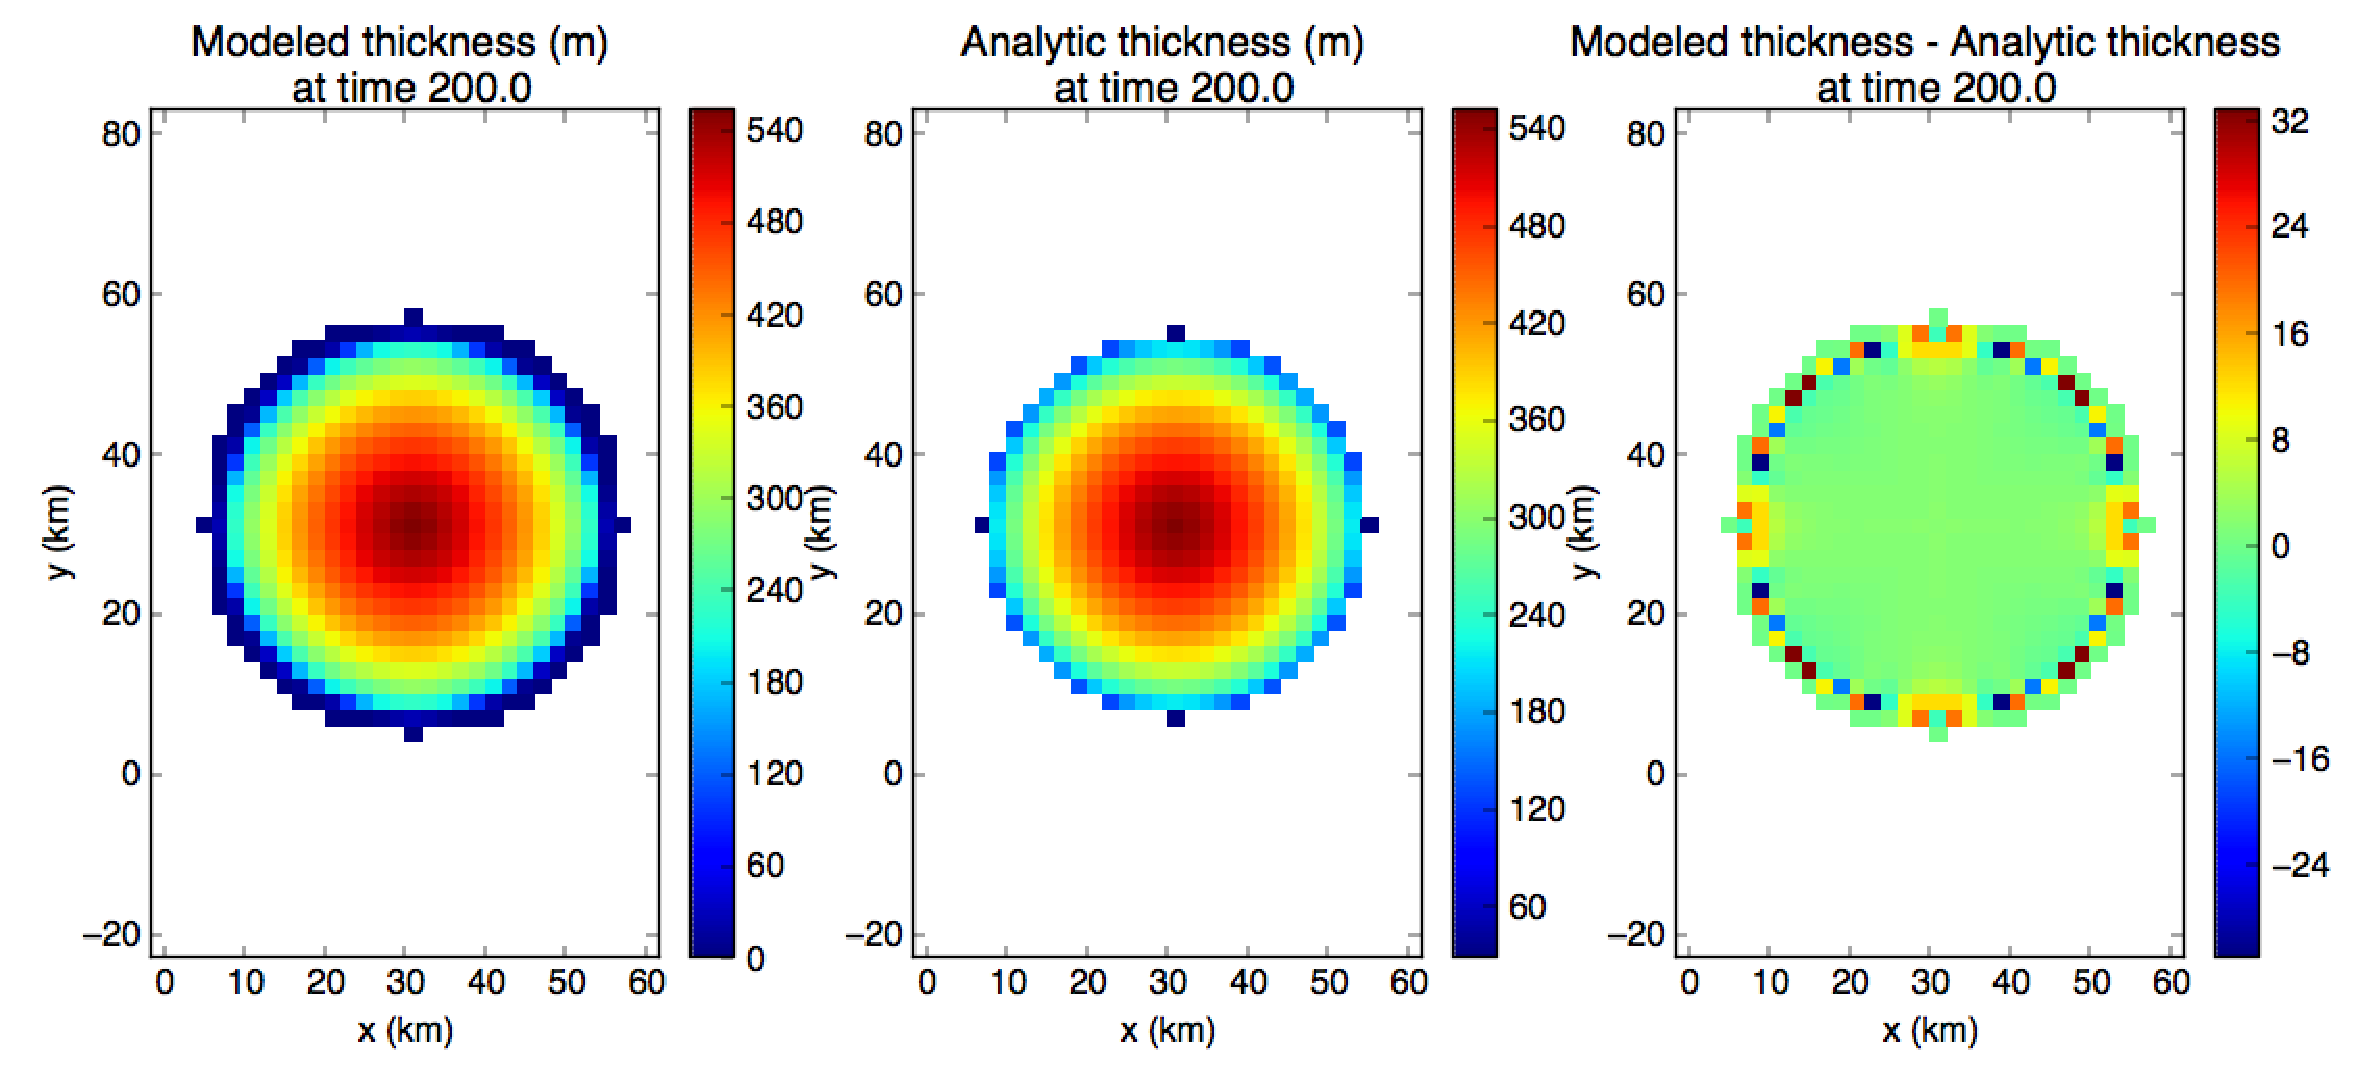
\includegraphics[width=16.4cm]{\dir/halfar_results.eps}
	\caption{Halfar test case results after 200 years of dome evolution. This figure is generated by \texttt{halfar\_results.py}.}
	\label{fig:halfarresults}
\end{figure}


\FloatBarrier


% =====================================
\subsection{EISMINT-1}
% =====================================
\label{sec:eismint_description}
This test case is from phase 1 of the European Ice Sheet Modelling INiTiative intercomparison experiments.  These experiments are described at \url{http://homepages.vub.ac.be/~phuybrec/eismint.html} and in \citet{Huybrechts1996}.

\subsubsection{Provided Files}
\label{subsec:eismint_files}

\begin{itemize}
	\item README \\
		Information about the test case, including technical details about running it.
\item *.config \\
  There are six .config files for each of the six experiments in EISMINT 1.  There are three fixed margin experiments (fm) and three moving margin experiments (mm).
\end{itemize}

\subsubsection{Running the test}
There is not a script for running these experiments.  They must be run manually, e.g.: 

\texttt{./cism\_driver e1-fm.1.config}


\subsubsection{Results}
\label{subsecc:eismint_results}
These experiments are meant to be run to steady-state, and the supplied .config files are setup to run for long enough for it to be reached.
These simulations take more than a few minutes to complete.
As the initial ice sheet evolves, its shape eventually reaches a steady-state with the imposed surface mass balance.  Currently there is not a script for analyzing the CISM results.  Users can manually compare their results to those in the \citet{Huybrechts1996} paper.


% =====================================
\subsection{EISMINT-2}
% =====================================
\label{sec:eismint2_description}
This test case is from phase 2 of the European Ice Sheet Modelling INiTiative intercomparison experiments.  These experiments are described at \url{http://homepages.vub.ac.be/~phuybrec/eismint.html} and in \citet{Payne2000}.

\subsubsection{Provided Files}
\label{subsec:eismint2_files}

\begin{itemize}
	\item README \\
		Information about the test case, including technical details about running it.
  \item *.config \\
  There are 11 .config files for each of the a-f experiments in EISMINT-2.
  \item mound.nc, trough.nc \\
    These are input netCDF files used by the EISMINT-2 experiments.
\end{itemize}

\subsubsection{Running the test}
There is not a script for running these experiments.  They must be run manually, e.g.: 

\texttt{./cism\_driver e2.a.config}


\subsubsection{Results}
\label{subsecc:eismint2_results}
These experiments are meant to be run to steady-state, and the supplied .config files are setup to run for long enough for it to be reached.  
Note that some of the experiments use the final state of a previous experiment 
as the initial condition.  See experiment descriptions in \citet{Payne2000} for details.
These simulations take more than a few minutes to complete.
As the initial ice sheet evolves, its shape eventually reaches a steady-state with the imposed surface mass balance.  Currently there is not a script for analyzing the CISM results.  Users can manually compare their results to those in the \citet{Payne2000} paper.


% =====================================
\subsection{GLINT example}
% =====================================
Glint example description

\subsubsection{Provided Files}

\begin{itemize}
	\item README \\
		Information about the test case, including technical details about running it.
\item ?.config \\
  ???
\item ???... \\
\end{itemize}

\subsubsection{Running the test}
There is not a script for running this experiment.  It must be run manually, e.g.: 

\texttt{./cism\_driver greenland\_20km.config glint\_example.config}

[describe the two .config syntax]

\subsubsection{Results}
???




% =====================================

\section{Higher-Order Test Cases}

Info here about running the various HO test cases.

\subsection{Dome}

\subsection{ISMIP-HOM}

\subsection{Confined Shelf}

\subsection{Circular Shelf}

\subsection{Ross Ice Shelf}




%% Old documentation below here, with edits are noted

%\chapter{User Guide (DEPRECATED)}
%\renewcommand{\dir}{ug}
%%% NOTE: this is the OLD documentation - most of these sections have been replaced with new equivalents
\label{ch:runcism}

\section{Overview of Running CISM}

Assuming you successfully completed the Installation instructions in Chapter \ref{chp:install},
the executable for running the model, \texttt{cism\_driver}, can be found in your 
build directory in a subdirectory called \texttt{cism\_driver} 
(e.g., \texttt{./builds/mac-gnu/cism\_driver/cism\_driver}).

The build system creates the executable at this path but does not automatically
make it available to other locations on your system.  How you choose to do so depends 
on your situation.  See the introduction to Chapter \ref{chp:testcases} for 
an overview of how to make the executable available to other locations on your system
(e.g., symlinking, copying, or modifying your PATH environment variable).

Unlike previous versions of Glimmer, with CISM 2.0 this single \texttt{cism\_driver} 
executable is used for running the model in all configurations.
\texttt{cism\_driver} can be invoked with a single argument specifying 
a CISM .config file to run CISM as a standalone ice sheet model without Glint climate forcing,
or with two arguments (a CISM config file and a Glint config file) 
to run CISM with Glint climate forcing:
\begin{verbatim}
 Call cism_driver with either 1 or 2 arguments. Examples:
 cism_driver ice_sheet.config
 cism_driver ice_sheet.config climate.config
\end{verbatim}
The available options for the CISM configuration file and 
for the Glint climate interface configuration file are described in detail below.

To perform a parallel run with the parallel build of CISM, you must use the
MPI run command, which is typically \texttt{mpirun} or \texttt{mpiexec} but may 
vary among MPI versions and installations.  A standard syntax that is likely to
work on most installations is \newline
 \indent \texttt{mpirun -np N cism\_driver ice\_sheet.config \textit{climate.config}} \newline
where \texttt{N} is the number of processors you want to use, \texttt{ice\_sheet.config} is the name of the CISM
configuration file, and the optional argument \texttt{\textit{climate.config}} is the name 
of the climate configuration file.  For example: \newline
 \indent \texttt{mpirun -np 4 cism\_driver dome.config}\newline
would run the dome test case on four processors.

Finally, note that instructions for running CISM within the Community Earth System Model (CESM)
or another climate model are not described here.

When CISM runs, some basic information about its operation will be output to 
the screen (standard out).  More verbose information about the run will be written 
to a log file which is named \texttt{\textit{ice\_sheet.config}.log} where 
\texttt{\textit{ice\_sheet.config}} is the name of the .config file use to perform
the run.  (For example, if running the model with  \texttt{./cism\_driver dome.config},
the log file will be called  \texttt{dome.config.log}.)  The log file is an
important reference, especially for debugging runs that do not behave as expected.
For example, the log file includes a list of configuration options and parameter
values, which can be useful in diagnosing problems like typos in your .config file.
The log file also indicates what files were used for input and output and at which
times I/O occurred.  The log file may contain warnings about potentially
problematic configuration combinations or model behavior, such as the use of
configurations settings that are not scientifically validated, or a CFL violation
during advection.  In contrast, fatal errors will kill the model and the error
message will be written to both the screen and the log file.

Optionally, the log file also contains diagnostic information about the global
state of the ice sheet (e.g., the total ice area and volume, the maximum surface and basal
speeds, and the max and min temperatures), along with vertical profiles of speed
and temperature at a user-specified grid point.  This information is written at intervals
specified by the config file variable \texttt{dt\_diag}, for the diagnostic
point \texttt{(idiag,jdiag)}.

In addition to the log file, the model will create any netCDF output files requested
in the config file (see Section \ref{io-config} below for details).  
If the model dies for some reason midway through a simulation,
the netCDF files will still include output for the portion of the simulation that 
was completed.

\section{Overview of Configuration Files}

Running CISM is managed through configuration files (*.config) that enable 
desired model features and control input of initial conditions and forcing 
and output of model results.  This chapter summarizes the configuration options 
available for running CISM and is divided into sections on general Model Configuration, 
Input/Ouput Configuration, and optional Climate Forcing Configuration.

The format of CISM configuration files is taken from that used by the 
ConfigParser module in Python 2.x, which is similar to Windows \texttt{.ini} files 
and contains sections. Each section contains key/value pairs.

\begin{itemize}
\item[Comments:] Empty lines, or lines starting with a \texttt{\#}, \texttt{;} or \texttt{!} are ignored.  Comments can also be added on the same line as a key/value pair using these delimiters.
\item[Sections:] A new section starts with the section name enclosed by square brackets, \texttt{[ ]} and can be up to 50 characters long, e.g., \texttt{[grid]}.
\item[Key/Value Pairs:] Keys are separated from their associated values by \texttt{=} or \texttt{:}. The names can be up to 50 characters long. Values can be up to 400 characters long.
\end{itemize}

Sections and keys are case-sensitive and may contain white space. 
However, the configuration parser is very simple and thus the number of spaces 
within a key or section name also matters. Sensible defaults are used when 
a specific key is not found; defaults are shown in bold in the tables below.

Here is an example configuration file:
\begin{verbatim}
;a comment
[a section]
an_int  : 1
a_float = 2.0
a_char  = hey, this is rather cool
an_array = 10. 20. -10. 40. 100.

[another section]
! more comments
foo : bar
\end{verbatim}




\input{\dir/installation.tex}
\section{GLIDE}
GLIDE is the actual ice sheet model. GLIDE comprises three procedures which initialise the model, perform a single time step and finalise the model. The GLIDE configuration file is described in Section \ref{ug.sec.config}. The GLIDE API is described in Appendix \ref{ug.sec.glide_api}. The simple example driver explains how to write a simple climate driver for GLIDE. Download the example from the GLIMMER website or from CVS:
\begin{verbatim}
cvs -d:pserver:anonymous@forge.nesc.ac.uk:/cvsroot/glimmer login
cvs -z3 -d:pserver:anonymous@forge.nesc.ac.uk:/cvsroot/glimmer co glimmer-example
\end{verbatim}

\subsection{Configuration}\label{ug.sec.config}
The format of the configuration files is taken from that used by the ConfigParser module in Python 2.x, which is similar to Windows \texttt{.ini} files and contains sections. Each section contains key, value(s) pairs.
\begin{itemize}
\item Empty lines, or lines starting with a \texttt{\#}, \texttt{;} or \texttt{!} are ignored.
\item A new section starts with the the section name enclose with square brackets, e.g. \texttt{[grid]}.
\item Keys are separated from their associated values by a \texttt{=} or \texttt{:}.
\end{itemize}
Sections and keys are case sensitive and may contain white space. However, the configuration parser is very simple and thus the number of spaces within a key or section name also matters. Sensible defaults are used when a specific key is not found.  Defaults are indicated in bold in the table below.

For consistency, options for both the shallow-ice and higher-order dynamical cores (dycore) are discussed. {\bf TODO: Keep this statement?} Currently, only the shallow ice dycore is scientifically supported. The higher-order dycore will be supported as part of planned future releases of Glimmer CISM. {\bf TODO: Keep this convention?} Configuration number options with a * after them are specific to the higher-order dycore.

\begin{center}
  \tablefirsthead{%
    \hline
  }
  \tablehead{%
    \hline
    \multicolumn{2}{|l|}{\emph{\small continued from previous page}}\\
    \hline
  }
  \tabletail{%
    \hline
    \multicolumn{2}{|r|}{\emph{\small continued on next page}}\\
    \hline}
  \tablelasttail{\hline}
  \begin{supertabular*}{\textwidth}{@{\extracolsep{\fill}}|l|p{10cm}|}


%%%% GRID
    \hline
    \multicolumn{2}{|l|}{\texttt{[grid]}}\\
    \hline
    \multicolumn{2}{|p{0.97\textwidth}|}{Define model grid. Maybe we should make this optional and read grid specifications from input netCDF file (if present). Certainly, the input netCDF files should be checked (but presently are not) if grid specifications are compatible.}\\
    \hline
    \texttt{ewn} & (integer) number of nodes in $x$--direction\\
    \texttt{nsn} & (integer) number of nodes in $y$--direction\\
    \texttt{upn} & (integer) number of nodes in $z$--direction\\
    \texttt{dew} & (real) node spacing in $x$--direction (m)\\
    \texttt{dns} & (real) node spacing in $y$--direction (m)\\
%% global_bc
    \texttt{global\_bc} & 
        boundary conditions for the edges of the global domain \\ &
    \begin{tabular}[t]{cp{0.85\linewidth}}
      {\bf 0} & periodic \\
      1 & outflow \\
    \end{tabular}\\
%    \texttt{sigma\_file} & (string) Name of file containing $\sigma$ coordinates. Alternatively, the sigma levels may be specified using the \texttt{[sigma]} section decribed below. If no sigma coordinates are specified explicitly, they are calculated based on the value of \texttt{sigma\_builtin} \\
    \texttt{sigma} &
%    \begin{tabular}[t]{cp{\linewidth}}
%      \multicolumn{2}{p{0.72\textwidth}}{If sigma coordinates are not specified in this configuration file or using the \texttt{sigma\_file} option, this specifies how to compute the sigma coordinates.} \\
      method for specifying sigma coordinates:  \\ &
    \begin{tabular}[t]{cl}
      {\bf 0} & Use Glimmer's default spacing \\[0.05in] 
        & $\sigma_i=\frac{1-(x_i+1)^{-n}}{1-2^{-n}}\quad\mbox{with}\quad x_i=\frac{\sigma_i-1}{\sigma_n-1}, n=2.$ \\[0.05in]
      1 & use sigma coordinates defined in external file (named sigma\_file) \\
      2 & use sigma coordinates given in configuration file \\
      3 & use evenly spaced sigma levels (required by Glam 1st-order dycore) \\
      4 & use Pattyn sigma levels \\
    \end{tabular}\\



%%%% SIGMA
    \hline
    \hline
    \hline
    \multicolumn{2}{|l|}{\texttt{[sigma]}}\\
    \hline
    \multicolumn{2}{|p{0.95\textwidth}|}{Define the sigma levels used in the vertical discretization (\texttt{sigma}=2 above). This is an alternative to using a separate file (specified in section \texttt{[grid]} above). If neither is used, the levels are calculated as described above.} \\
    \hline
    \texttt{sigma\_levels} & (real) list of sigma levels, in ascending order, separated by spaces. These run between 0.0 and 1.0 \\



%%%% TIME
    \hline
    \hline
    \hline
    \multicolumn{2}{|l|}{\texttt{[time]}}\\
    \hline
    \multicolumn{2}{|p{0.95\textwidth}|}{Configure time steps, etc. {\bf TODO: Address/remove this note:} Update intervals should probably become absolute values rather than related to the main time step when we introduce variable time steps.}\\
    \hline
    \texttt{tstart} & (real) Start time of the model in years\\
    \texttt{tend} & (real) End time of the model in years\\
    \texttt{dt} & (real) size of time step in years\\
    \texttt{subcyc} & (integer) number of time steps to subcycle within dt using a steady velocity field {\bf TODO: Support both subcyc and ntem/nvel?  Explain the difference?}\\
    \texttt{ntem} & (real) time step multiplier setting the ice temperature update interval\\
    \texttt{nvel} & (real) time step multiplier setting the velocity update interval\\
    \texttt{profile} & (integer) profile frequency (number of time steps) {\bf TODO: more useful description of what profiling is?}\\
    \texttt{dt\_diag} & (real) writing diagnostic variables to log file every dt\_diag yrs\\
    \texttt{idiag} & (int) x direction grid index for diagnostic variables to be written to log file\\
    \texttt{jdiag} & (int) y direction grid index for diagnostic variables to be written to log file\\
    \texttt{ndiag} & (int) number of time steps between diagnostics. {\bf DEPRECATED}.  Use \texttt{dt\_diag}.\\



%%%% Options
    \hline
    \hline
    \hline
    \multicolumn{2}{|l|}{\texttt{[options]}}\\
    \hline
    \multicolumn{2}{|p{0.95\textwidth}|}{Parameters set in this section determine how various components of the ice sheet model are treated.}\\
    \hline
%% dycore
    \texttt{dycore} & 
      {\bf TODO: Add Felix, Bisicles?} \\ &
    \begin{tabular}[t]{cp{0.85\linewidth}}
      {\bf 0} & Glide (serial, 3d, Shallow-Ice-Approximation dynamical core)\\
      1* & Glam (parallel, 3d, FDM, 1st-order-accurate dynamical core)  \\
      2* & Glissade (parallel, 3d, FEM, 1st-order-accurate dynamical core)  \\
    \end{tabular}\\
%% evolution
    \texttt{evolution} & 
    \begin{tabular}[t]{ll}
      {\bf 0} & pseudo-diffusion (Glide only)\\
      1 & ADI scheme  (Glide only)\\
      2 & diffusion (Glide only)\\
      3* & incremental remapping (Glam/Glissade only) \\
      4* & first-order upwind (Glam/Glissade only) \\
      5* & evolve without changing ice thickness (Glam/Glissade only) \\
    \end{tabular}\\
%% temperature
    \texttt{temperature} & 
    \begin{tabular}[t]{cl}
      0 & Set each ice column to local surface air temperature \\
      {\bf 1} & prognostic temperature calculation \\
      2 & held steady at initial value \\
      3 & prognostic temperature calculation using enthalpy formulation {\bf TODO: include this?} \\
    \end{tabular}\\
%% temperature init
    \texttt{temp\_init} & 
    \begin{tabular}[t]{cp{0.85\linewidth}}
      0 & initial temperatures isothermal at 0 deg. C\\
      {\bf 1} & initial column temperatures set to atmos. temperature \\
      2 & initial column temperatures linearly interpolated from atmos. temperature \\
    \end{tabular}\\
%% flow law
    \texttt{flow\_law} &  
    \begin{tabular}[t]{cp{0.85\linewidth}}
      {\bf 0}  & constant (using the value of default\_flwa)\\
      1 & temp. dependent, Patterson and Budd (temp.=-5degC)\\
      2 & temp. dependent, Patterson and Budd (function of variable temp.)\\
    \end{tabular}\\
%% basal water
    \texttt{basal\_water} & 
    \begin{tabular}[t]{cp{0.85\linewidth}}
      {\bf 0} & none \\
      1 & local water balance\\
      2 & Compute the steady-state, routing-based, basal water flux and water layer thickness \\
      3 &  Use a constant basal water layer thickness everywhere, to enforce T=T\_pmp everywhere \\
    \end{tabular}\\
%% basal mass balance
    \texttt{basal\_mass\_balance} & 
    \begin{tabular}[t]{cl}
      {\bf 0} & ignore basal melt rate in mass balance calculation \\
      1 & include basal melt rate in mass balance calculation \\
    \end{tabular}\\
%% slip coefficient
    \texttt{slip\_coeff} & 
        slip coefficient for Glide only \\ &
    \begin{tabular}[t]{cl}
      {\bf 0} & zero (no sliding) \\
      1 & set to a non--zero constant everywhere\\
      2 & set to constant where basal water (bwat) is nonzero\\
      3 & set to constant where the ice base is melting\\
      4 & set proportional to basal melt rate\\
      5 & Tanh function of basal water (bwat)\\
    \end{tabular}\\
%% marine margin
    \texttt{marine\_margin} & 
  {\bf TODO: KEEP ALL OF THESE?} \\ &
    \begin{tabular}[t]{cp{0.85\linewidth}}
      0 & ignore marine margin\\
      {\bf 1} & Set thickness to zero if floating\\
      2 & Lose fraction of ice when edge cell\\
      3 & Set thickness to zero if relaxed bedrock is below a given depth (variable "mlimit" in glide\_types)\\
      4 & Set thickness to zero if present-day bedrock is below a given depth (variable "mlimit" in glide\_types)\\
      5 & Huybrechts grounding line scheme {\bf TODO: elaborate on this.} \\
    \end{tabular}\\
%% vertical integration
    \texttt{vertical\_integration} & 
    \begin{tabular}[t]{cp{0.85\linewidth}}
      {\bf 0} & standard integration\\
      1 & constrained so that upper boundary kinematic velocity is obeyed\\
    \end{tabular}\\
%% geothermal heat flux
    \texttt{gthf} &  
    \begin{tabular}[t]{cp{0.85\linewidth}}
      {\bf 0} & prescribed, uniform geothermal heat flux \\
      1 & read 2d geothermal heat flux field from input file \\
      2 & calculate geothermal heat flux using 3d diffusion model \\
    \end{tabular}\\
%% isostasy
    \texttt{isostasy} &  
    \begin{tabular}[t]{cp{0.85\linewidth}}
      {\bf 0} & no isostatic adjustment \\
      1 & compute isostatic adjustment using lithosphere / asthenosphere model \\
    \end{tabular}\\
%% topography
    \texttt{topo\_is\_relaxed} &  
    \begin{tabular}[t]{cp{0.85\linewidth}}
      {\bf 0} & relaxed topography is read from a separate variable\\
      1 & first time slice of input topography is assumed to be relaxed\\
      2 & first time slice of input topography is assumed to be in isostatic
      equilibrium with ice thickness. \\
    \end{tabular}\\
%% periodicity
    \texttt{periodic\_ew} & 
  {\bf TODO: Is this still used?  If so, do we need to add perdiodic\_ns?} \\&
    \begin{tabular}[t]{cp{0.85\linewidth}}
      {\bf 0} & switched off\\
      1 & periodic lateral EW boundary conditions (Glide SIA dycore only) \\
    \end{tabular}\\
%% restart
    \texttt{restart} &
    Note: the alternate keyword {\bf hotstart} is retained for backwards compatibility. \\ &
    \begin{tabular}[t]{cp{0.85\linewidth}}
      {\bf 0} & normal start (initial guesses taken from input file or, if absent, using default options)\\
      1 & restart model using input from previous run (do not calc., e.g., temp., rate factor, or vel. fields)  
           Specific fields required for restart or dependent on options chosen.  (Specify 'restart' as a variable 
           in an output file to get the required fields automatically.)\\
    \end{tabular}\\
    \hline
    \texttt{ioparams} & (string) name of file containing netCDF I/O configuration. The main configuration file is searched for I/O related sections if no file name is given (default).\\



 %%%% HIGHER-ORDER OPTIONS
    \hline
    \hline
    \hline
    \multicolumn{2}{|l|}{\texttt{[ho\_options]}}\\
    \hline
    \multicolumn{2}{|p{0.95\textwidth}|}{Options set in this section determine how various components of the higher-order extensions to the ice sheet model are treated. Defaults are indicated in bold. As noted above, higher-order model options are currently NOT scientifically supported.}\\
    \hline
%% which_ho_nonlinear
    \texttt{which\_ho\_nonlinear} & 
    \begin{tabular}[t]{cp{0.85\linewidth}}
      {\bf 0} & treat nonlinearity in momentum balance using Picard iteration \\
      1 & treat nonlinearity in momentum balance using Jacobian-Free Newton-Krylov iteration  \\
    \end{tabular}\\     
%% which_ho_sparse
    \texttt{which\_ho\_sparse} & 
{\bf TODO: Bill, check these descriptions for accuracy?  Also, do we need notes about which options are glissade vs. glam specific?} \\ &
    \begin{tabular}[t]{cp{0.85\linewidth}}
      -1 & Solve sparse linear system using SLAP library with incomplete Cholesky method\\
      {\bf 0} & Solve sparse linear system with incomplete LU-preconditioned biconjugate gradient method\\
      1 & Solve sparse linear system with incomplete LU-preconditioned GMRES method\\
      2 & Solve sparse linear system with conjugate gradient method (parallel code only)\\
      3 & Solve sparse linear system with conjugate gradient method with Chronopoulos-Gear preconditioner (parallel code only)\\
      4 & Solve sparse linear system using Trilinos, incomplete LU-preconditioned GMRES method (Trilinos compatible build only)\\
    \end{tabular}\\     
%% which_ho_efvs
    \texttt{which\_ho\_efvs} & 
    \begin{tabular}[t]{cp{0.85\linewidth}}
      0 & use a constant value for the effective viscosity: 2336041.42829 Pa yr (Value used by ISMIP-HOM Test F)\\
      1 & set the effective viscosity to a value based on the flow rate factor: efvs $= 0.5 * A^{-1/n}$\\
      {\bf 2} & use the effective strain rate for the calc. of the effective viscosity (i.e., full nonlinear treatment) \\
    \end{tabular}\\  
%% which_disp
    \texttt{which\_disp} & 
{\bf TODO: Should this be moved from ho\_options to options?} \\ &
    \begin{tabular}[t]{cp{0.85\linewidth}}
      {\bf 0} & calculate dissipation in temperature equation assuming SIA ice dynamics \\
      1* & calculate dissipation in temperature equation assuming 1st-order ice dynamics \\
    \end{tabular}\\    
%% which_ho_babc
    \texttt{which\_ho\_babc} & 
        Implementation of basal boundary condition in higher-order dycore (Calculation of `beta' field.) {\bf TODO: include all of these?} \\ &
    \begin{tabular}[t]{cp{0.85\linewidth}}
      0 & constant value \\
      1 & specify some simple pattern (hardcoded). Useful for debugging\\
      2 & read yield stress (in Pa) from input field `mintauf' to simulate sliding 
          over a plastic subglacial till (using Picard iteration)\\
      3 & calculate `beta' as linear (inverse) function of basal water thickness\\
      {\bf 4} & no slip everywhere in domain (`beta' set to very
          large value)\\
      5 & read value of `beta' in from .nc input file using standard i/o \\
      6 & no slip everywhere in domain (using Dirichlet basal BC)\\
      7 & read yield stress (in Pa) from input field `mintauf' to simulate sliding 
          over a plastic subglacial till (using Newton iteration - under devel.)\\
      8 & Spatial field of `beta' required for ISMIP-HOM Test C \\
    \end{tabular}\\  
%% which_ho_resid
    \texttt{which\_ho\_resid} &
     Residual calculation method for the velocity solver in higher-order dycore
     (iterations halt once residual falls below a specified absolute or relative value) \\ &
    \begin{tabular}[t]{cp{0.85\linewidth}}
      0 & use the maximum value of the normalized velocity vector update, defined by 
      $r = \frac{|vel_{k-1} - vel_k|}{vel_k}$ \\
      1 & as in option 0 but omitting the basal velocities from the comparison
          (useful in cases where an approx. no slip basal BC is enforced) \\
      2 & as in option 0 but using the mean rather than the max \\
      {\bf 3} & use the L2 norm of the system residual, defined by $r = Ax - b$ \\
    \end{tabular}\\  
%% which_ho_approx
    \texttt{which\_ho\_approx} &
     Which Stokes approximation to use with the glissade dycore \\ &
    \begin{tabular}[t]{cp{0.85\linewidth}}
      -1 & Shallow-ice approximation, Glide-type calculation (uses glissade\_velo\_sia) \\
      0 & Shallow-ice approximation, vertical-shear stresses only (uses glissade\_velo\_higher) \\
      1 & Shallow-shelf approximation, horizontal-plane stresses only (uses glissade\_velo\_higher) \\
      {\bf 2} & Blatter-Pattyn with both vertical-shear and horizontal-plane stresses (uses glissade\_velo\_higher) \\
    \end{tabular}\\  
%% which_ho_precond
    \texttt{which\_ho\_precond} &
     Which Stokes preconditioner to use in the glissade dycore \\ &
    \begin{tabular}[t]{cp{0.85\linewidth}}
      0 & No preconditioner \\
      1 & Diagonal preconditioner \\
      {\bf 2} & Physics-based shallow-ice preconditioner \\
    \end{tabular}\\  
%% which_ho_gradient
    \texttt{which\_ho\_gradient} &
     Which gradient operator to use in the glissade dycore \\ &
    \begin{tabular}[t]{cp{0.85\linewidth}}
      0 & Centered gradient \\
      {\bf 1} & Upstream gradient {\bf TODO: Make sure this has been set as the default in the code (currently default is 0)}\\
    \end{tabular}\\  


 %%%% EXTERNAL DYCORE OPTIONS
    \hline
    \hline
    \hline
    \multicolumn{2}{|l|}{\texttt{[external\_dycore\_options]}}\\
    \hline
    \multicolumn{2}{|p{0.95\textwidth}|}{Options set in this section are specific to external dycores that 
    may have additional options/option files.  {\bf TODO: include this stuff?  elaborate?} }\\
    \hline
%% external_dycore_type
    \texttt{external\_dycore\_type} & 
    \begin{tabular}[t]{cp{0.85\linewidth}}
      1 & Use BISICLES external dycore \\
      2 & Use Albany-FELIX external dycore \\
    \end{tabular}\\     
    \texttt{dycore\_input\_file} &
    Specify path to additional configuration file required by the external dycore. \\



%%%% PARAMETERS
    \hline
    \hline
    \hline
    \multicolumn{2}{|l|}{\texttt{[parameters]}}\\
    \hline
    \multicolumn{2}{|p{0.95\textwidth}|}{Set values for various parameters.}\\
    \hline
    \texttt{log\_level} & (integer) set to a value between 0, no messages, and 6, all messages are displayed to stdout. By default messages are only logged to file.\\
    \texttt{ice\_limit} & (real) below this limit ice is only accumulated/ablated; ice dynamics are switched on once the ice thickness is above this value. (default = 100.0 m) \\
    \texttt{ice\_limit\_temp} & (real) minimum thickness for computing vertical temperature (m). (default = 1.0 m) \\
    \texttt{marine\_limit} & (real) all ice is assumed lost once water depths reach this value (for \texttt{marine\_margin}=3 or 4 in \texttt{[options]} above). Note, water depth is negative.  (default = -200.0 m) \\
    \texttt{calving\_fraction} & (real) fraction of ice lost due to calving (applies to "marine\_margin" option 2). (default = 0.8)\\
    \texttt{geothermal} & (real) constant geothermal heat flux. (default = -0.05 W m$^{-2}$)\\
    \texttt{flow\_factor} & (real) the flow law is enhanced with this factor (default = 3.0)\\
     \texttt{default\_flwa} * & Flow law parameter A to use in isothermal experiments (flow\_law set to 0).  Default value is $10^{-16}$ Pa$^{-n}$ yr$^{-1}$. \\
    \texttt{hydro\_time} & (real) basal hydrology time constant (default = 1000.0 yr) \\
    \texttt{basal\_tract\_const} & constant basal traction parameter. You can load a nc file with a variable called \texttt{soft} if you want a spatially varying bed softness parameter. \\
    \texttt{basal\_tract\_max} & Max value for basal traction when using \texttt{slip\_coeff}=4. \\
    \texttt{basal\_tract\_slope} & Slope value for basal traction relation when using \texttt{slip\_coeff}=4. (Relation also uses \texttt{basal\_tract\_const}.)\\
    \texttt{basal\_tract\_tanh} & (real(5)) basal traction factors. Basal traction is set to $B=\tanh(W)$ where the parameters
      \begin{tabular}{cp{\linewidth}}
       (1) & width of the $\tanh$ curve\\
       (2) & $W$ at midpoint of $\tanh$ curve [m]\\
       (3) & $B$ minimum [ma$^{-1}$Pa$^{-1}$] \\
       (4) & $B$ maximum [ma$^{-1}$Pa$^{-1}$] \\
       (5) & multiplier for marine sediments \\
     \end{tabular}\\
    \texttt{ho\_beta\_const} * & (real) spatially uniform beta used when \texttt{which\_ho\_babc} = 0. (default = 10.0 Pa yr m$^{-1}$) \\
    \texttt{periodic\_offset\_ew} & (real) Vertical offset between east and west edges of the global domain. (default = 0.0 m)  (Primarily used for ISMIP-HOM test cases.) \\
    \texttt{periodic\_offset\_ns} & (real) Vertical offset between north and south edges of the global domain. (default = 0.0 m)  (Primarily used for ISMIP-HOM test cases.)\\



%%%% GTHF
    \hline
    \hline
    \hline
    \multicolumn{2}{|l|}{\texttt{[GTHF]}}\\
    \hline
    \multicolumn{2}{|p{0.95\textwidth}|}{Options related to lithospheric temperature and geothermal heat calculation.  Ignored unless \texttt{gthf} = 1.}\\
    \hline
    \texttt{num\_dim} & can be either \texttt{1} for 1D calculations or 3 for 3D calculations.\\
    \texttt{nlayer} & number of vertical layers (default: 20). \\
    \texttt{surft} & initial surface temperature (default 2$^\circ$C).\\
    \texttt{rock\_base} & depth below sea-level at which geothermal heat gradient is applied (default: -5000m).\\
    \texttt{numt} & number time steps for spinning up GTHF calculations (default: 0).\\
    \texttt{rho} & The density of lithosphere (default: 3300kg m$^{-3}$).\\
    \texttt{shc} & specific heat capcity of lithosphere (default: 1000J kg$^{-1}$ K$^{-1}$).\\
    \texttt{con} & thermal conductivity of lithosphere (3.3 W m$^{-1}$ K$^{-1}$).\\    



%%%% ISOSTASY
    \hline
    \hline
    \hline
    \multicolumn{2}{|l|}{\texttt{[isostasy]}}\\
    \hline
    \multicolumn{2}{|p{0.95\textwidth}|}{Options related to isostasy model.  Ignored unless \texttt{isostasy} = 1.  {\bf TODO: Need comments about which combinations are valid.} }\\
    \hline
    \texttt{lithosphere} & \begin{tabular}[t]{cp{0.9\linewidth}} 
      {\bf 0} & local lithosphere, equilibrium bedrock depression is found using Archimedes' principle \\
      1 & elastic lithosphere, flexural rigidity is taken into account
    \end{tabular} \\
    \texttt{asthenosphere} & \begin{tabular}[t]{cp{\linewidth}}
      {\bf 0} & fluid mantle, isostatic adjustment happens instantaneously \\
      1 & relaxing mantle, mantle is approximated by a half-space \\
    \end{tabular} \\    
    \texttt{relaxed\_tau} & characteristic time constant of relaxing mantle (default: 4000.a) \\
    \texttt{update} & lithosphere update period (default: 500.a) \\
    \hline
%%%%
%    \hline
%    \multicolumn{2}{|l|}{\texttt{[elastic lithosphere]}}\\
%    \hline
%    \multicolumn{2}{|p{0.95\textwidth}|}{Set up parameters of the elastic lithosphere.}\\
    \hline
    \texttt{flexural\_rigidity} & flexural rigidity of the lithosphere (default: 0.24e25)\\



%%%% PROJECTION
    \hline
    \hline
    \hline
    \multicolumn{2}{|l|}{\texttt{[projection]}}\\
    \hline
    \multicolumn{2}{|p{0.95\textwidth}|}{Specify map projection. The reader is
    referred to Snyder J.P. (1987) \emph{Map Projections - a working manual.} USGS 
        Professional Paper 1395.    {\bf TODO: I am assuming this works.  Code is not in glide\_setup.F90.  Appears to be in glimmap\_printproj() in ../libglimmer/glimmer\_map\_init.F90}}\\
    \hline
    \texttt{type} & This is a string that specifies the projection type
    (\texttt{LAEA}, \texttt{AEA}, \texttt{LCC} or \texttt{STERE}). \\
    \texttt{centre\_longitude} & Central longitude in degrees east \\
    \texttt{centre\_latitude} & Central latitude in degrees north \\
    \texttt{false\_easting} & False easting in meters \\
    \texttt{false\_northing} & False northing in meters \\
    \texttt{standard\_parallel} & Location of standard parallel(s) in degrees
    north. Up to two standard parallels may be specified (depending on the
    projection). \\
    \texttt{scale\_factor} & non-dimensional. Only relevant for the Stereographic projection.  \\




  \end{supertabular*}
\end{center}

NetCDF I/O can be configured in the main configuration file or in a separate file 
(see \texttt{ioparams} in the \texttt{[options]} section). 
Any number of input, forcing, and output files can be specified. 

Input files are processed in the same order they occur in the configuration file, 
thus potentially overwriting previously loaded fields.  The configuration section 
for an input file specified which time slice from the input file should be used as
the initial condition.  (Note this is an integer specifying the time level, not
the actual time.)

Forcing files are new in CISM 2.0 and are input files that are read on every 
time step to allow time-dependent
forcing to be applied during a simulation.  Any inputtable fields can be included
in forcing files.  Forcing files should have a ``time'' field which is used to 
assign values to each field in the file during the simulation.  Forcing is applied 
in a piecewise constant fashion -- the most recent time slice in the forcing file prior
to the current model time is used on each time step.  (Linearly interpolatation of
forcing may be available in the future but is not currently implemented.)
Note that if a field is present in both an input file and in a
forcing file at the start time, the value in the forcing file will overwrite the value
from the input file because forcing files get read after input files.
Forcing files are processed in the same order they occur in the configuration file, 
on each time step thus potentially overwriting previously loaded fields from other
forcing files.

\begin{center}
  \tablefirsthead{%
    \hline
  }
  \tablehead{%
    \hline
    \multicolumn{2}{|l|}{\emph{\small continued from previous page}}\\
    \hline
  }
  \tabletail{%
    \hline
    \multicolumn{2}{|r|}{\emph{\small continued on next page}}\\
    \hline}
  \tablelasttail{\hline}
  \begin{supertabular*}{\textwidth}{@{\extracolsep{\fill}}|l|p{11cm}|}
%%%% CF defaults
    \hline
    \multicolumn{2}{|l|}{\texttt{[CF default]}}\\
    \hline
    \multicolumn{2}{|p{0.95\textwidth}|}{This section contains metadata describing the experiment. Any of these parameters can be modified in the \texttt{[output]} section. The model automatically attaches a time stamp and the model version to the netCDF output file.}\\
    \hline
    \texttt{title}& Title of the experiment\\
    \texttt{institution} & Institution at which the experiment was run\\
    \texttt{references} & References that might be useful\\
    \texttt{comment} & A comment, further describing the experiment\\
    \hline

%%%% CF Input
    \hline
    \hline
    \hline
    \multicolumn{2}{|l|}{\texttt{[CF input]}}\\
    \hline
    \multicolumn{2}{|p{0.95\textwidth}|}{Any number of input files can be specified in separate \texttt{[CF input]} sections. They are processed in the order they occur in the configuration file, potentially overriding previously loaded variables.}\\
    \hline
    \texttt{name}& The name of the netCDF file to be read. Typically netCDF files end with \texttt{.nc}.\\
    \texttt{time}& The time slice (not actual time) to be read from the netCDF file. The first time slice is read by default.\\
    \hline

%%%% CF Forcing
    \hline
    \hline
    \hline
    \multicolumn{2}{|l|}{\texttt{[CF forcing]}}\\
    \hline
    \multicolumn{2}{|p{0.95\textwidth}|}{Any number of forcing files can be specified in separate \texttt{[CF forcing]} sections. They are processed in the order they occur in the configuration file, potentially overriding previously loaded variables.  Each forcing file needs a ``time'' dimension and variable that indicates the model time associated with each time slice in the file. }\\
    \hline
    \texttt{name}& The name of the netCDF file to be read. Typically netCDF files end with \texttt{.nc}.\\
    \hline

%%%% CF output
    \hline
    \hline
    \hline
    \multicolumn{2}{|l|}{\texttt{[CF output]}}\\
    \hline
    \multicolumn{2}{|p{0.95\textwidth}|}{This section of the netCDF parameter file controls how often selected  variables are written to file.}\\
    \hline
    \texttt{name} & The name of the output netCDF file. Typically netCDF files end with \texttt{.nc}.\\
    \texttt{start} & Start writing to file when this time is reached (default: first time slice).\\
    \texttt{stop} & Stop writin to file when this time is reached (default: last time slice). \\
    \texttt{frequency} & The time interval in years, determining how often selected variables are written to file.\\
    \texttt{xtype} & Set the floating point representation used in netCDF file. \texttt{xtype} can be one of \texttt{real}, \texttt{double} (default: \texttt{real}). \\
    \texttt{variables} & List of variables to be written to file. See Appendix \ref{ug.sec.varlist} for a list of known variables. Names should be separated by at least one space. The variable names are case sensitive. Variable \texttt{restart} selects all variables necessary for a restart.\\
    \hline
  \end{supertabular*}
\end{center}

\input{\dir/drivers.tex}
\input{\dir/glint.tex}
\input{\dir/mbals.tex}
`

%\chapter{Tutorial (DEPRECATED)}
%\renewcommand{\dir}{tut}
%** The only relevant text from here, the use of glint-example, was moved into the section describing glint (Climate Forcing section of ``running cism" chapter) **

%\label{ch:runcism}

\section{Overview of Running CISM}

Assuming you successfully completed the Installation instructions in Chapter \ref{chp:install},
the executable for running the model, \texttt{cism\_driver}, can be found in your 
build directory in a subdirectory called \texttt{cism\_driver} 
(e.g., \texttt{./builds/mac-gnu/cism\_driver/cism\_driver}).

The build system creates the executable at this path but does not automatically
make it available to other locations on your system.  How you choose to do so depends 
on your situation.  See the introduction to Chapter \ref{chp:testcases} for 
an overview of how to make the executable available to other locations on your system
(e.g., symlinking, copying, or modifying your PATH environment variable).

Unlike previous versions of Glimmer, with CISM 2.0 this single \texttt{cism\_driver} 
executable is used for running the model in all configurations.
\texttt{cism\_driver} can be invoked with a single argument specifying 
a CISM .config file to run CISM as a standalone ice sheet model without Glint climate forcing,
or with two arguments (a CISM config file and a Glint config file) 
to run CISM with Glint climate forcing:
\begin{verbatim}
 Call cism_driver with either 1 or 2 arguments. Examples:
 cism_driver ice_sheet.config
 cism_driver ice_sheet.config climate.config
\end{verbatim}
The available options for the CISM configuration file and 
for the Glint climate interface configuration file are described in detail below.

To perform a parallel run with the parallel build of CISM, you must use the
MPI run command, which is typically \texttt{mpirun} or \texttt{mpiexec} but may 
vary among MPI versions and installations.  A standard syntax that is likely to
work on most installations is \newline
 \indent \texttt{mpirun -np N cism\_driver ice\_sheet.config \textit{climate.config}} \newline
where \texttt{N} is the number of processors you want to use, \texttt{ice\_sheet.config} is the name of the CISM
configuration file, and the optional argument \texttt{\textit{climate.config}} is the name 
of the climate configuration file.  For example: \newline
 \indent \texttt{mpirun -np 4 cism\_driver dome.config}\newline
would run the dome test case on four processors.

Finally, note that instructions for running CISM within the Community Earth System Model (CESM)
or another climate model are not described here.

When CISM runs, some basic information about its operation will be output to 
the screen (standard out).  More verbose information about the run will be written 
to a log file which is named \texttt{\textit{ice\_sheet.config}.log} where 
\texttt{\textit{ice\_sheet.config}} is the name of the .config file use to perform
the run.  (For example, if running the model with  \texttt{./cism\_driver dome.config},
the log file will be called  \texttt{dome.config.log}.)  The log file is an
important reference, especially for debugging runs that do not behave as expected.
For example, the log file includes a list of configuration options and parameter
values, which can be useful in diagnosing problems like typos in your .config file.
The log file also indicates what files were used for input and output and at which
times I/O occurred.  The log file may contain warnings about potentially
problematic configuration combinations or model behavior, such as the use of
configurations settings that are not scientifically validated, or a CFL violation
during advection.  In contrast, fatal errors will kill the model and the error
message will be written to both the screen and the log file.

Optionally, the log file also contains diagnostic information about the global
state of the ice sheet (e.g., the total ice area and volume, the maximum surface and basal
speeds, and the max and min temperatures), along with vertical profiles of speed
and temperature at a user-specified grid point.  This information is written at intervals
specified by the config file variable \texttt{dt\_diag}, for the diagnostic
point \texttt{(idiag,jdiag)}.

In addition to the log file, the model will create any netCDF output files requested
in the config file (see Section \ref{io-config} below for details).  
If the model dies for some reason midway through a simulation,
the netCDF files will still include output for the portion of the simulation that 
was completed.

\section{Overview of Configuration Files}

Running CISM is managed through configuration files (*.config) that enable 
desired model features and control input of initial conditions and forcing 
and output of model results.  This chapter summarizes the configuration options 
available for running CISM and is divided into sections on general Model Configuration, 
Input/Ouput Configuration, and optional Climate Forcing Configuration.

The format of CISM configuration files is taken from that used by the 
ConfigParser module in Python 2.x, which is similar to Windows \texttt{.ini} files 
and contains sections. Each section contains key/value pairs.

\begin{itemize}
\item[Comments:] Empty lines, or lines starting with a \texttt{\#}, \texttt{;} or \texttt{!} are ignored.  Comments can also be added on the same line as a key/value pair using these delimiters.
\item[Sections:] A new section starts with the section name enclosed by square brackets, \texttt{[ ]} and can be up to 50 characters long, e.g., \texttt{[grid]}.
\item[Key/Value Pairs:] Keys are separated from their associated values by \texttt{=} or \texttt{:}. The names can be up to 50 characters long. Values can be up to 400 characters long.
\end{itemize}

Sections and keys are case-sensitive and may contain white space. 
However, the configuration parser is very simple and thus the number of spaces 
within a key or section name also matters. Sensible defaults are used when 
a specific key is not found; defaults are shown in bold in the tables below.

Here is an example configuration file:
\begin{verbatim}
;a comment
[a section]
an_int  : 1
a_float = 2.0
a_char  = hey, this is rather cool
an_array = 10. 20. -10. 40. 100.

[another section]
! more comments
foo : bar
\end{verbatim}




%\input{\dir/gex.tex}
%\input{\dir/gtest.tex}
%\input{\dir/glint.tex}


%\part{Developer Documentation}

%\chapter{Numerics (DEPRECATED)}
%\renewcommand{\dir}{num}
%\input{\dir/num.tex}

%\chapter{Developer Guide (DEPRECATED)}
%** The useful info in here, relevant to things that we still support, has all been moved elsewhere **
%\renewcommand{\dir}{dg}
%\input{\dir/dg.tex}

%% SP: we removed support for the "extensions", and they weren't coming up in the pdf for some reason anyway
%\renewcommand{\dir}{ext}
%\input{\dir/ext.tex}

\part{Appendix}
\label{ch:appendix}
\appendix
\renewcommand{\dir}{ug}
\chapter{NetCDF Variables}
\label{ch:appendix_vars}
\label{ug.sec.varlist}
The following list shows all the netCDF variable names used by CISM. 
Only variables marked with $^\ast$ are loaded (if present) by the input routines.
\section{Glide/Glissade Variables}
\input{\dir/glide_varlist.tex}
%\section{EIS Variables}
%** We're not supporting EIS, so commented this out of build **
%\input{\dir/eis_varlist.tex}
\section{Glint Variables}
\input{\dir/glint_varlist.tex}

%** Commented out the stuff on the GLIMMER API for now **
%WHL - I agree that we don't need this in the new doc.
%\chapter{The GLIMMER API}
%\input{\dir/glum_api.tex}
%\input{\dir/glide_api.tex}
%\input{\dir/glint_api.tex}
\renewcommand{\dir}{ext}
\input{\dir/ext-app.tex}

%\chapter{Configuration File}
%\renewcommand{\dir}{dg}
%\input{\dir/config_file.tex}

\chapter{Input and Output (I/O)}
\label{ch:appendix_io}
\renewcommand{\dir}{dg}
\input{\dir/netcdf.tex}

\chapter{Commonly Used Notation}
\label{ch:notation}
\renewcommand{\dir}{appendix}
The following table is a partial list of the notation for commonly used variables in this document.


\begin{center}
    \tablefirsthead{%
    \hline
        Symbol &  Variable\\
    \hline
    \hline}
  \tablehead{%
    \hline
    \multicolumn{3}{|p{0.98\textwidth}|}{\emph{\small continued from previous page}}\\
    \hline
        Symbol &  Variable\\
    \hline
    \hline}
  \tabletail{%
    \hline
    \multicolumn{3}{|r|}{\emph{\small continued on next page}}\\
    \hline}
  \tablelasttail{\hline}
  \begin{supertabular}{|l|p{8cm}|c|}
    \hline

\ $H$   &    ice thickness  \\
\hline

\ $s$   &    ice surface elevation  \\
\hline

\ $b$   &    ice bottom elevation  \\
\hline

\ $b_r$   &    bedrock elevation  \\
\hline

\ $B_s$   &    surface mass balance  \\
\hline

\ $B_b$   &    basal mass balance  \\
\hline

\ $B$   &    combined surface and basal mass balance  \\
\hline

\ $u$   &    x-component of ice velocity  \\
\hline

\ $v$   &    y-component of ice velocity  \\
\hline

\ $w$   &    z-component of ice velocity  \\
\hline

\ $\eta$   &    effective viscosity  \\
\hline


  \end{supertabular}
\end{center}





\part{Bibliography}
\bibliography{glimmer}
\end{document}
